\documentclass[a4paper,12pt]{ctexart}

\usepackage{geometry}
\usepackage{amsmath}
\usepackage{amssymb}
\usepackage{xcolor}

% Force graphicx to use final mode and display real figures
\usepackage[final]{graphicx}
\setkeys{Gin}{draft=false}

% Figure directory
\graphicspath{{pic/}{./pic/}}

% Accepted graphics extensions
\DeclareGraphicsExtensions{.png,.jpg,.jpeg,.pdf}

\usepackage{multirow}
\usepackage{fancyhdr}
\usepackage{float}
\usepackage{subcaption}
\usepackage{booktabs}
\usepackage{tabularx}
\usepackage{array}
\usepackage{longtable}
\usepackage{bm}
\usepackage[hidelinks]{hyperref}
\usepackage[numbers,sort&compress]{natbib}

\geometry{left=2.5cm, right=2.5cm, top=2.5cm, bottom=2.5cm}

\renewcommand{\figurename}{Figure}
\renewcommand{\abstractname}{Abstract}
\numberwithin{equation}{section}
\renewcommand{\theequation}{\thesection.\arabic{equation}}

\pagestyle{fancy}
\fancyhf{}
\fancyfoot[C]{\thepage}

\newcommand{\vb}[1]{\bm{#1}}
\newcommand{\vx}{\vb{x}}
\newcommand{\vn}{\vb{n}}
\newcommand{\vs}{\vb{s}}
\newcommand{\vq}{\vb{q}}
\newcommand{\vc}{\vb{c}}
\newcommand{\vxi}{\bm{\xi}}
\newcommand{\dd}{\mathrm{d}}
\newcommand{\figwidth}{0.32\textwidth}
\newcommand{\TODO}[1]{\textcolor{red}{TODO: #1}}
\newcounter{procedure}
\renewcommand{\theprocedure}{\arabic{procedure}}

\makeatletter
\renewcommand\maketitle{
\begin{center}
\vspace*{1cm}
\LARGE\bfseries \@title
\par\vskip 0.5em
\large \@author
\par\vskip 0.8cm
\end{center}
}
\makeatother

\begin{document}

\title{A coupled DUGKS for transient conduction–radiation in participating media}

\begin{abstract}
Transient heat transfer in participating media requires the simultaneous resolution of thermal diffusion and angular radiative transport, yet these processes are often advanced by different numerical schemes. Here, a coupled discrete unified gas-kinetic scheme (DUGKS) is developed for gray, absorbing, emitting, and isotropically scattering media. A temperature distribution function represents the energy equation, whereas a pseudo-time kinetic relaxation equation resolves the radiative intensity. Both fields share a single control-volume grid, and their interface fluxes are reconstructed from characteristic solutions. This arrangement evaluates the radiative source directly at the temperature nodes and avoids interpolation between separate thermal and radiative meshes. The formulation is assessed using literature-derived one-dimensional planar and two-dimensional square benchmarks over selected scattering albedos and conduction--radiation parameters. Recomputed DUGKS results agree with reference temperature and heat-flux data for the slab and square-enclosure cases, capture the transition from radiation-dominated to conduction-dominated transport, and resolve the slower heating associated with stronger scattering. The calculations also show that radiative heat flux requires finer angular resolution than temperature. The coupled framework therefore provides a consistent finite-volume kinetic approach for transient conduction--radiation simulations and a basis for extensions to non-gray media and complex geometries.
\end{abstract}

\section{Introduction}
\label{sec:introduction}

Heat transfer in high-temperature participating media depends on the interaction between thermal diffusion and radiative transport. This interaction governs thermal protection systems, combustion chambers, insulation layers, and radiatively active enclosures. Numerical prediction is difficult because the energy equation contains a radiative source, whereas the radiative transfer equation (RTE) contains emission proportional to $T^4$. The resulting coupling is nonlinear, nonlocal, and sensitive to optical thickness, scattering albedo, the conduction--radiation parameter, and geometry. One-dimensional slabs provide a standard benchmark for transient conduction--radiation coupling~\cite{Talukdar2001}. Transient finite-element analyses further illustrate the numerical demands of coupled radiative heat transfer~\cite{Feng2021}. Extensions to anisotropically scattering cylinders and high-temperature media show the additional influence of geometry and coupling strategy~\cite{YasongSun2021,Zhu2024}.

Numerical studies have therefore relied widely on hybrid treatments of the energy equation and the RTE. Early work combined LBM heat conduction with the discrete transfer method~\cite{MishraLankadasu2005} or with an FVM radiation solver~\cite{MishraRoy2007}. Other formulations coupled LBM with the discrete ordinates method~\cite{MondalMishra2007} or adopted a shared-grid LBM--FVM treatment for planar and square media~\cite{Sun2016}. The same benchmark family includes short-time slab solutions~\cite{Sutton1986}, transient scattering calculations~\cite{LinTsai1990}, and two-dimensional rectangular or square enclosures~\cite{YuenTakara1988,WuOu1994}. This route was subsequently extended to irregular geometries and composite or graded materials~\cite{Abaszadeh2022,Tong2022}. Related models treated graded-index media~\cite{Wei2023} and curved radiative boundaries~\cite{Sharifi2023}. Unstructured radiation models and complex-geometry LBM--FVM algorithms broadened the available spatial discretisations~\cite{Liu2024,Miao2025}. These methods offer accuracy and geometric flexibility. However, they generally advance thermal diffusion and radiative transport through distinct numerical mechanisms.

The discrete unified gas-kinetic scheme (DUGKS) offers a route to reduce this separation. The original DUGKS reconstructs finite-volume interface fluxes from characteristic solutions of the governing kinetic equation~\cite{Guo2013}. Wang et al. subsequently coupled separate velocity and temperature distributions for Boussinesq flows~\cite{Wang2015}. Characteristic reconstruction incorporates transport and relaxation into flux evaluation, while the time step follows a CFL condition rather than fixed lattice streaming. The finite-volume kinetic framework was later extended to conjugate heat transfer~\cite{Tao2021} and immersed-boundary fluid-solid thermal coupling~\cite{Tao2022}. Further developments addressed non-Oberbeck--Boussinesq convection~\cite{Wen2025} and complex thermal flows on hierarchical Cartesian grids~\cite{Tao2025}.

Gas-kinetic schemes have also advanced radiative-transfer modelling. Unified gas-kinetic schemes were first developed for gray RTEs~\cite{SunJiangXu2015} and then extended to frequency-dependent transport~\cite{Sun2015Frequency}. Multidimensional formulations supported unstructured radiation meshes~\cite{Sun2017}, while DUGKS enabled multiscale radiative heat-transfer calculations~\cite{Luo2018}. Later work introduced positive asymptotic-preserving moment treatments~\cite{Xu2021} and accelerated steady DUGKS iterations~\cite{Song2022}. Diffusion synthetic acceleration improved steady radiative calculations~\cite{Song2023}, whereas spatially second-order schemes strengthened accuracy and asymptotic preservation~\cite{Xu2023}. Positive formulations were subsequently extended to nonlinear radiative transfer~\cite{Xu2024,Song2025}. Cylindrical-coordinate systems~\cite{Wang2025Cyl} and three-temperature radiation models~\cite{Li2025} further broadened their scope. Positivity-preserving gray RTE schemes continue to refine kinetic flux construction~\cite{Wang2026}. Collectively, these studies establish gas-kinetic schemes as credible RTE solvers. However, a common DUGKS treatment of thermal and radiative updates in transient benchmarks remains underexplored.

The present study addresses this gap with a coupled DUGKS for transient conduction--radiation heat transfer in gray participating media. A temperature distribution function represents the energy equation, and a pseudo-time kinetic relaxation equation advances the radiative intensity. Both fields are solved on the same control-volume grid. The radiative source is evaluated directly at temperature nodes, while both fluxes are obtained through characteristic reconstruction. This unified treatment avoids interpolation between separate thermal and radiative meshes. The formulation is assessed by recomputing representative slab and square-enclosure cases selected from the above literature. The resulting benchmark matrix includes pointwise literature comparisons, transient temperature profiles, heat-flux decomposition, scattering-albedo sweeps, conduction--radiation-parameter sweeps, and angular-resolution tests.

\section{Coupled DUGKS formulation for conduction--radiation heat transfer}
\label{sec:coupled_dugks}

The coupled DUGKS uses kinetic representations of temperature and radiative intensity. The following derivation specifies their evolution equations, angular discretisation, boundary treatment, and coupling procedure.

\subsection{Gas-kinetic model for transient conduction--radiation problems}
\label{subsec:kinetic_model}

The participating medium is gray, absorbing, emitting, and isotropically scattering. The density $\rho$, specific heat $c_p$, thermal conductivity $k$, absorption coefficient $\kappa_a$, and scattering coefficient $\kappa_s$ are constant. Because the benchmark configurations exclude fluid motion, the macroscopic model contains only the transient energy equation and the RTE. The dimensional energy equation is
\begin{equation*}
\rho c_p\frac{\partial T}{\partial t}=k\nabla^2T-\nabla\cdot\vq_r,
\end{equation*}
where $T$ denotes temperature and $\vq_r$ denotes radiative heat flux. For a gray medium with isotropic scattering, the radiative-flux divergence is
\begin{equation*}
\nabla\cdot\vq_r=\beta(1-\omega)\left(4\sigma T^4-G_d\right),
\end{equation*}
where $\beta=\kappa_a+\kappa_s$ is the extinction coefficient, $\omega=\kappa_s/\beta$ is the scattering albedo, and $\sigma$ is the Stefan--Boltzmann constant. The quantity $G_d$ is the dimensional incident radiation. The RTE along direction $\vs$ is
\begin{equation*}
\vs\cdot\nabla I=-\beta I+\kappa_a I_b+\frac{\kappa_s}{4\pi}\int_{4\pi}I(\vs')\dd\Omega',
\end{equation*}
where $I=I(\vx,\vs)$ is the directional radiation intensity and $I_b=\sigma T^4/\pi$ is the blackbody intensity.

The characteristic length is $L$, and the hot-wall temperature $T_w$ defines the reference temperature. Using the thermal diffusivity $\alpha=k/(\rho c_p)$, the dimensionless variables are
\begin{equation*}
\begin{aligned}
\theta&=\frac{T}{T_w},\\
\vx^*&=\frac{\vx}{L},\\
\zeta&=\frac{\alpha t}{L^2},\\
G&=\frac{G_d}{4\sigma T_w^4}.
\end{aligned}
\end{equation*}
The optical thickness is $\tau_L=\beta L$, and the conduction--radiation parameter is
\begin{equation*}
N=\frac{\kappa_a k}{4\sigma T_w^3}.
\end{equation*}
The dimensionless energy equation is
\begin{equation}
\begin{aligned}
\frac{\partial\theta}{\partial\zeta}&=\nabla^2\theta+Q_r,
\\
Q_r&=\frac{1-\omega}{N}\left(G-\theta^4\right),
\end{aligned}
\label{eq:dimensionless_energy}
\end{equation}
where $Q_r$ is the dimensionless radiative source. Small $N$ indicates strong radiative exchange relative to conduction, whereas large $N$ corresponds to a conduction-dominated regime.

To represent Eq.~\eqref{eq:dimensionless_energy} within DUGKS, a temperature distribution function $g=g(\vx,\vxi,t)$ is introduced. With zero macroscopic velocity, its kinetic equation is
\begin{equation}
\begin{aligned}
\frac{\partial g}{\partial t}+\vxi\cdot\nabla g&=\Omega^g+S^g,
\\
\Omega^g&=\frac{g^{eq}-g}{\tau_g},
\end{aligned}
\label{eq:thermal_kinetic_continuous}
\end{equation}
where $\tau_g$ is the thermal relaxation time. The equilibrium and radiative-source distributions are
\begin{equation*}
\begin{aligned}
g^{eq}&=\theta\,\mathcal{M}(\vxi),
\\
S^g&=Q_r\,\mathcal{M}(\vxi),
\end{aligned}
\end{equation*}
where $\mathcal{M}$ is a normalised weight function. The zeroth moment of Eq.~\eqref{eq:thermal_kinetic_continuous} recovers the energy equation because $\int\Omega^g\dd\vxi=0$ and $\int S^g\dd\vxi=Q_r$.

The steady RTE is solved through a pseudo-time kinetic relaxation equation. For each angular control volume, indexed by $m$, the dimensionless intensity $I_m$ satisfies
\begin{equation}
\begin{aligned}
\frac{\partial I_m}{\partial \chi}+\vs_m\cdot\nabla I_m&=\Omega_m^I,
\\
\Omega_m^I&=\frac{I_m^{eq}-I_m}{\tau_I},
\end{aligned}
\label{eq:radiation_kinetic}
\end{equation}
where $\chi$ is pseudo time and $\tau_I$ is the radiative relaxation time. The present calculations use $\tau_I=1$. The equilibrium intensity is
\begin{equation}
I_m^{eq}=(1-\omega)\theta^4+\omega G.
\label{eq:radiation_equilibrium}
\end{equation}
Angular moments of the intensity give the incident radiation and radiative heat flux,
\begin{equation}
\begin{aligned}
G&=\sum_{m=1}^{M}w_m I_m,
\\
\vq_r&=\sum_{m=1}^{M}w_m\vs_m I_m,
\end{aligned}
\label{eq:angular_moments}
\end{equation}
where $w_m$ is the angular quadrature weight. For the one-dimensional slab, the zenith interval $[0,\pi]$ is divided into $M=16$ angular control volumes. Over an interval $[\theta_l,\theta_r]$, the quadrature weight and representative direction cosine are
\begin{equation*}
\begin{aligned}
w_m&=\frac{1}{2}(\cos\theta_l-\cos\theta_r),
\\
\mu_m&=\frac{1}{2}(\cos\theta_l+\cos\theta_r).
\end{aligned}
\end{equation*}
The corresponding directional heat-flux weight is
\begin{equation*}
w_m^q=\frac{1}{4}(\sin^2\theta_r-\sin^2\theta_l).
\end{equation*}
For the two-dimensional square enclosure, polar and azimuthal control volumes discretise the solid angle. The angular data contain the projected directions $(\mu_{x,m},\mu_{y,m})$, solid-angle weights $w_m$, and heat-flux weights used along the centreline. A CFL condition based on the largest projected transport speed determines the pseudo-time step. Equations~\eqref{eq:thermal_kinetic_continuous} and \eqref{eq:radiation_kinetic} form the coupled kinetic model. The radiation equation depends on local emission $\theta^4$, whereas the temperature equation depends on $G$ through $Q_r$.

\subsection{DUGKS for the temperature field}
\label{subsec:temperature_dugks}

The computational domain is divided into finite-volume cells $V_j$ centred at $\vx_j$. After discretisation of velocity space by $\vxi_i$, the temperature kinetic equation becomes
\begin{equation}
\begin{aligned}
\frac{\partial g_i}{\partial t}+\vxi_i\cdot\nabla g_i&=\Omega_i^g+S_i^g,
\\
\Omega_i^g&=\frac{g_i^{eq}-g_i}{\tau_g},
\\
S_i^g&=w_i Q_r,
\end{aligned}
\label{eq:thermal_kinetic_discrete}
\end{equation}
where $w_i$ is the velocity quadrature weight. Without macroscopic motion, the equilibrium distribution is
\begin{equation*}
g_i^{eq}=w_i\theta.
\end{equation*}
Equation~\eqref{eq:thermal_kinetic_discrete} is integrated over $V_j$ from $t_n$ to $t_{n+1}$. Applying midpoint integration to the flux and trapezoidal integration to the collision and source terms gives
\begin{equation}
\tilde g_{i,j}^{n+1}=\tilde g_{i,j}^{+,n}-\frac{\Delta t}{|V_j|}F_{i,j}^{n+1/2},
\label{eq:g_update}
\end{equation}
where
\begin{equation}
\begin{aligned}
F_{i,j}^{n+1/2}&=\int_{\partial V_j}(\vxi_i\cdot\vn)g_i(\vx,t_n+h)\,\dd S,
\\
h&=\frac{\Delta t}{2}.
\end{aligned}
\label{eq:g_flux}
\end{equation}
The auxiliary distributions are defined by
\begin{equation*}
\begin{aligned}
\tilde g_i&=g_i-\frac{\Delta t}{2}\left(\Omega_i^g+S_i^g\right),
\\
\tilde g_i^+&=g_i+\frac{\Delta t}{2}\left(\Omega_i^g+S_i^g\right).
\end{aligned}
\end{equation*}
Because the collision term has zero zeroth moment, the macroscopic temperature is recovered from
\begin{equation}
\theta=\sum_i\tilde g_i+\frac{\Delta t}{2}Q_r.
\label{eq:temperature_from_tilde}
\end{equation}
The source $Q_r$ is evaluated from the latest converged radiation field. For implicit treatment of $\theta^4$, Eq.~\eqref{eq:temperature_from_tilde} is solved by local fixed-point iteration. Otherwise, a second-order explicit prediction provides $Q_r$.

The central DUGKS step evaluates the interface distribution $g_i(\vx_b,t_n+h)$ in Eq.~\eqref{eq:g_flux}. Equation~\eqref{eq:thermal_kinetic_discrete} is integrated over a half time step ending at interface $\vx_b$. Introducing
\begin{equation*}
\begin{aligned}
\bar g_i&=g_i-\frac{h}{2}\left(\Omega_i^g+S_i^g\right),
\\
\bar g_i^+&=g_i+\frac{h}{2}\left(\Omega_i^g+S_i^g\right),
\end{aligned}
\end{equation*}
gives
\begin{equation*}
\bar g_i(\vx_b,t_n+h)=\bar g_i^+(\vx_b-\vxi_i h,t_n).
\end{equation*}
For smooth solutions, a Taylor expansion about the upwind cell centre $\vx_c$ reconstructs the right-hand side,
\begin{equation}
\bar g_i^+(\vx_b-\vxi_i h,t_n)
\approx \bar g_i^+(\vx_c,t_n)+\nabla\bar g_i^+(\vx_c,t_n)\cdot(\vx_b-\vxi_i h-\vx_c),
\label{eq:g_reconstruction}
\end{equation}
where a gradient limiter can suppress nonphysical oscillations.

The physical interface distribution is recovered from $\bar g_i$ as
\begin{equation*}
g_i(\vx_b,t_n+h)=\frac{2\tau_g}{2\tau_g+h}\bar g_i(\vx_b,t_n+h)
+\frac{h}{2\tau_g+h}g_i^{eq}(\vx_b,t_n+h)
+\frac{\tau_g h}{2\tau_g+h}S_i^g(\vx_b,t_n+h).
\end{equation*}
The corresponding post-collision variables are
\begin{equation}
\bar g_i^+=\frac{2\tau_g-h}{2\tau_g+\Delta t}\tilde g_i
+\frac{3h}{2\tau_g+\Delta t}g_i^{eq}
+\frac{3h\tau_g}{2\tau_g+\Delta t}S_i^g,
\label{eq:g_bar_plus}
\end{equation}
\begin{equation}
\tilde g_i^+=\frac{4}{3}\bar g_i^+-\frac{1}{3}\tilde g_i.
\label{eq:g_tilde_plus}
\end{equation}
Here, the source term is the radiative heat source $Q_r$. This coupling distinguishes the formulation from thermal DUGKS models driven by buoyancy alone.

The one-dimensional slab uses the D1Q3 velocity set,
\begin{equation*}
\begin{aligned}
\vxi_i&\in \{0, c_t, -c_t\},
\\
w_i&\in \left\{ \frac{2}{3}, \frac{1}{6}, \frac{1}{6} \right\}.
\end{aligned}
\end{equation*}
The two-dimensional square medium uses the D2Q9 tensor-product set. The relaxation time is selected to recover the dimensionless thermal diffusivity,
\begin{equation*}
\alpha^*=\tau_g RT=1,
\end{equation*}
where $RT$ is the lattice temperature of the discrete velocity set.

Non-equilibrium extrapolation imposes the thermal boundary condition. Each unknown incoming distribution contains an equilibrium part prescribed at the wall and a non-equilibrium part extrapolated from the adjacent cell. For a generic distribution $\phi_\ell$, representing either $g_i$ or $I_m$, this treatment is
\begin{equation}
\begin{aligned}
\phi_\ell(\vx_w)&=\phi_\ell^{eq}(\vx_w;\Psi_w)+\left[\phi_\ell(\vx_f)-\phi_\ell^{eq}(\vx_f;\Psi_f)\right],
\\
\vc_\ell\cdot\vn_{in}&>0,
\end{aligned}
\label{eq:nee_boundary}
\end{equation}
Here, $\vx_w$ is the boundary face and $\vx_f$ is the nearest interior cell centre. The variables $\Psi_w$ and $\Psi_f$ denote the prescribed wall quantity and its interior counterpart. The vector $\vc_\ell$ represents either thermal velocity $\vxi_i$ or radiative direction $\vs_m$. For the temperature field, $\Psi_w$ is the prescribed wall temperature. Equation~\eqref{eq:nee_boundary} enters the DUGKS update during reconstruction at boundary-adjacent faces.

\subsection{DUGKS for the radiative intensity field}
\label{subsec:radiation_dugks}

The RTE is first discretised in angular space. For direction $\vs_m$, Eq.~\eqref{eq:radiation_kinetic} is integrated over cell $V_j$ and pseudo-time step $\Delta\chi$. With $h_r=\Delta\chi/2$, the DUGKS update is
\begin{equation}
\tilde I_{m,j}^{n+1}=\tilde I_{m,j}^{+,n}-\frac{\Delta\chi}{|V_j|}\mathcal{F}_{m,j}^{n+1/2},
\label{eq:I_update}
\end{equation}
where
\begin{equation*}
\mathcal{F}_{m,j}^{n+1/2}=\int_{\partial V_j}(\vs_m\cdot\vn)I_m(\vx,\chi_n+h_r)\,\dd S.
\end{equation*}
The auxiliary radiative intensities are
\begin{equation}
\begin{aligned}
\tilde I_m&=I_m-\frac{\Delta\chi}{2}\Omega_m^I,
\\
\tilde I_m^+&=I_m+\frac{\Delta\chi}{2}\Omega_m^I,
\end{aligned}
\label{eq:I_tilde}
\end{equation}
\begin{equation*}
\begin{aligned}
\bar I_m&=I_m-\frac{h_r}{2}\Omega_m^I,
\\
\bar I_m^+&=I_m+\frac{h_r}{2}\Omega_m^I.
\end{aligned}
\end{equation*}
The transformed distributions satisfy
\begin{equation*}
\bar I_m^+=\frac{2\tau_I-h_r}{2\tau_I+\Delta\chi}\tilde I_m
+\frac{3h_r}{2\tau_I+\Delta\chi}I_m^{eq},
\end{equation*}
\begin{equation*}
\tilde I_m^+=\frac{4}{3}\bar I_m^+-\frac{1}{3}\tilde I_m.
\end{equation*}
The auxiliary interface intensity is reconstructed along the radiative characteristic,
\begin{equation}
\bar I_m(\vx_b,\chi_n+h_r)=\bar I_m^+(\vx_b-\vs_m h_r,\chi_n),
\label{eq:I_characteristic}
\end{equation}
and the physical interface intensity is
\begin{equation}
I_m(\vx_b,\chi_n+h_r)=\frac{2\tau_I}{2\tau_I+h_r}\bar I_m(\vx_b,\chi_n+h_r)
+\frac{h_r}{2\tau_I+h_r}I_m^{eq}(\vx_b,\chi_n+h_r).
\label{eq:I_interface}
\end{equation}

Because $I_m^{eq}$ contains the incident radiation $G$, this moment must be recovered from the auxiliary intensity. Taking the angular moment of Eq.~\eqref{eq:I_tilde} gives
\begin{equation}
G=\frac{\sum_m w_m\tilde I_m+\frac{\Delta\chi}{2\tau_I}(1-\omega)\theta^4}
{1+\frac{\Delta\chi}{2\tau_I}(1-\omega)}.
\label{eq:G_from_tilde}
\end{equation}
After recovering $G$, Eq.~\eqref{eq:radiation_equilibrium} updates $I_m^{eq}$, and the physical intensity is
\begin{equation*}
I_m=\frac{2\tau_I}{2\tau_I+\Delta\chi}\tilde I_m+\frac{\Delta\chi}{2\tau_I+\Delta\chi}I_m^{eq}.
\end{equation*}
The physical intensity then yields the radiative flux in Eq.~\eqref{eq:angular_moments}. Pseudo-time iteration continues until $G$ converges for the current temperature field. At radiative boundaries, Eq.~\eqref{eq:nee_boundary} prescribes the black or diffuse-gray equilibrium intensity. Its non-equilibrium correction is extrapolated from the adjacent interior cell.

Each physical time step contains a radiation stage followed by a temperature stage.

During the radiation stage, the radiative intensity equation is iterated in pseudo time at fixed temperature. Equation~\eqref{eq:G_from_tilde} first recovers $G$, and Eq.~\eqref{eq:radiation_equilibrium} updates $I_m^{eq}$. Equations~\eqref{eq:I_characteristic} and \eqref{eq:I_interface} then reconstruct the interface intensity before Eq.~\eqref{eq:I_update} advances the auxiliary intensity. This cycle continues until the incident radiation converges.

During the temperature stage, Eq.~\eqref{eq:dimensionless_energy} evaluates $Q_r$ from the converged radiation field. Equations~\eqref{eq:g_bar_plus} and \eqref{eq:g_tilde_plus} construct the auxiliary temperature distributions. Equation~\eqref{eq:g_reconstruction}, together with Eq.~\eqref{eq:nee_boundary}, reconstructs the interface distribution before Eq.~\eqref{eq:g_update} advances the temperature field.

The two stages repeat until the coupled field reaches steady state. Both equations share one control-volume grid, so the radiative source is evaluated directly at temperature nodes. Their interface fluxes are both reconstructed from DUGKS characteristic solutions.

\section{Results}
\label{sec:results}

The coupled DUGKS was evaluated using a one-dimensional planar medium and a two-dimensional square enclosure. Both benchmarks combine heat diffusion, wall emission, volumetric absorption, and angular radiative transport while permitting direct comparison of temperature and heat-flux profiles.

Unless stated otherwise, all material properties were constant, the optical thickness in each coordinate direction was unity, and all walls were black and diffuse.

\subsection{1D cases}
\label{subsec:1d_cases}

The one-dimensional domain was a slab of thickness $L$, represented by $0\leq X\leq 1$. The slab was initially at a uniform temperature $T_E$. At $t\geq0$, the left-wall temperature was raised to $T_w>T_E$ and held constant, while the right wall remained at $T_E$. The medium then approached steady state through combined conduction and radiation.

The energy equation and RTE were solved on the same cell-centred finite-volume mesh. Consequently, $G$, $Q_r$, and $T$ were evaluated at coincident locations. The zenith direction was divided into 16 angular control volumes. The tests examined scattering at $N=0.01$, variations in $N$ at $\omega=0$, and decomposition of the total heat flux into conductive and radiative components. Before the transient profile study, the method was first applied to the black-wall slab benchmark used by Sutton~\cite{Sutton1986}, Lin and Tsai~\cite{LinTsai1990}, Talukdar and Mishra~\cite{Talukdar2001}, Mishra and Roy~\cite{MishraRoy2007}, and Mondal and Mishra~\cite{MondalMishra2007}. Table~\ref{tab:slab_validation} reproduces the original comparison matrix compiled by Sun and Zhang~\cite{Sun2016}. Their own LBM--FVM solution is included as a separate reference row, followed by the present DUGKS result for direct comparison. This case used $\tau_L=1.0$, $\omega=0.5$, $T_E=0$, $N=0.1$, and $\zeta=0.05$.

\begin{table}[H]
\centering
\scriptsize
\caption{Dimensionless temperature in the one-dimensional slab benchmark at $\tau_L=1.0$, $\omega=0.5$, $T_E=0$, $N=0.1$, and $\zeta=0.05$. The original comparison data and the LBM--FVM solution are taken from Sun and Zhang~\cite{Sun2016}; the present DUGKS results are listed immediately after the LBM--FVM reference.}
\label{tab:slab_validation}
\resizebox{\textwidth}{!}{%
\begin{tabular}{@{}cc l ccc@{}}
\toprule
$\varepsilon_W$ & $\varepsilon_E$ & Investigator/method & $X=0.25$ & $X=0.50$ & $X=0.75$ \\
\midrule
\multirow{7}{*}{1.0} & \multirow{7}{*}{1.0} & Sutton~\cite{Sutton1986} & 0.4888 & 0.1778 & 0.0591 \\
& & Lin and Tsai~\cite{LinTsai1990}           & 0.4889 & 0.1773 & 0.0588 \\
& & Talukdar and Mishra~\cite{Talukdar2001}   & 0.4892 & 0.1768 & 0.0585 \\
& & Mishra and Roy~\cite{MishraRoy2007}       & 0.4897 & 0.1771 & 0.0587 \\
& & Mondal and Mishra~\cite{MondalMishra2007} & 0.4898 & 0.1769 & 0.0583 \\
& & LBM--FVM (Sun and Zhang)~\cite{Sun2016}   & 0.4894 & 0.1771 & 0.0585 \\
& & Present DUGKS                              & 0.4912 & 0.1782 & 0.0590 \\
\bottomrule
\end{tabular}%
}
\end{table}

Table~\ref{tab:slab_validation} shows that the present DUGKS reproduces the pointwise temperature levels reported by the established slab benchmarks. Relative to the LBM--FVM results of Sun and Zhang~\cite{Sun2016}, the maximum absolute difference is $1.8\times10^{-3}$. The remaining differences are small relative to the spread among the published reference values and are consistent with differences in spatial, angular, and boundary discretisation.

\begin{figure}[H]
\centering
\begin{subfigure}[b]{\figwidth}
\centering
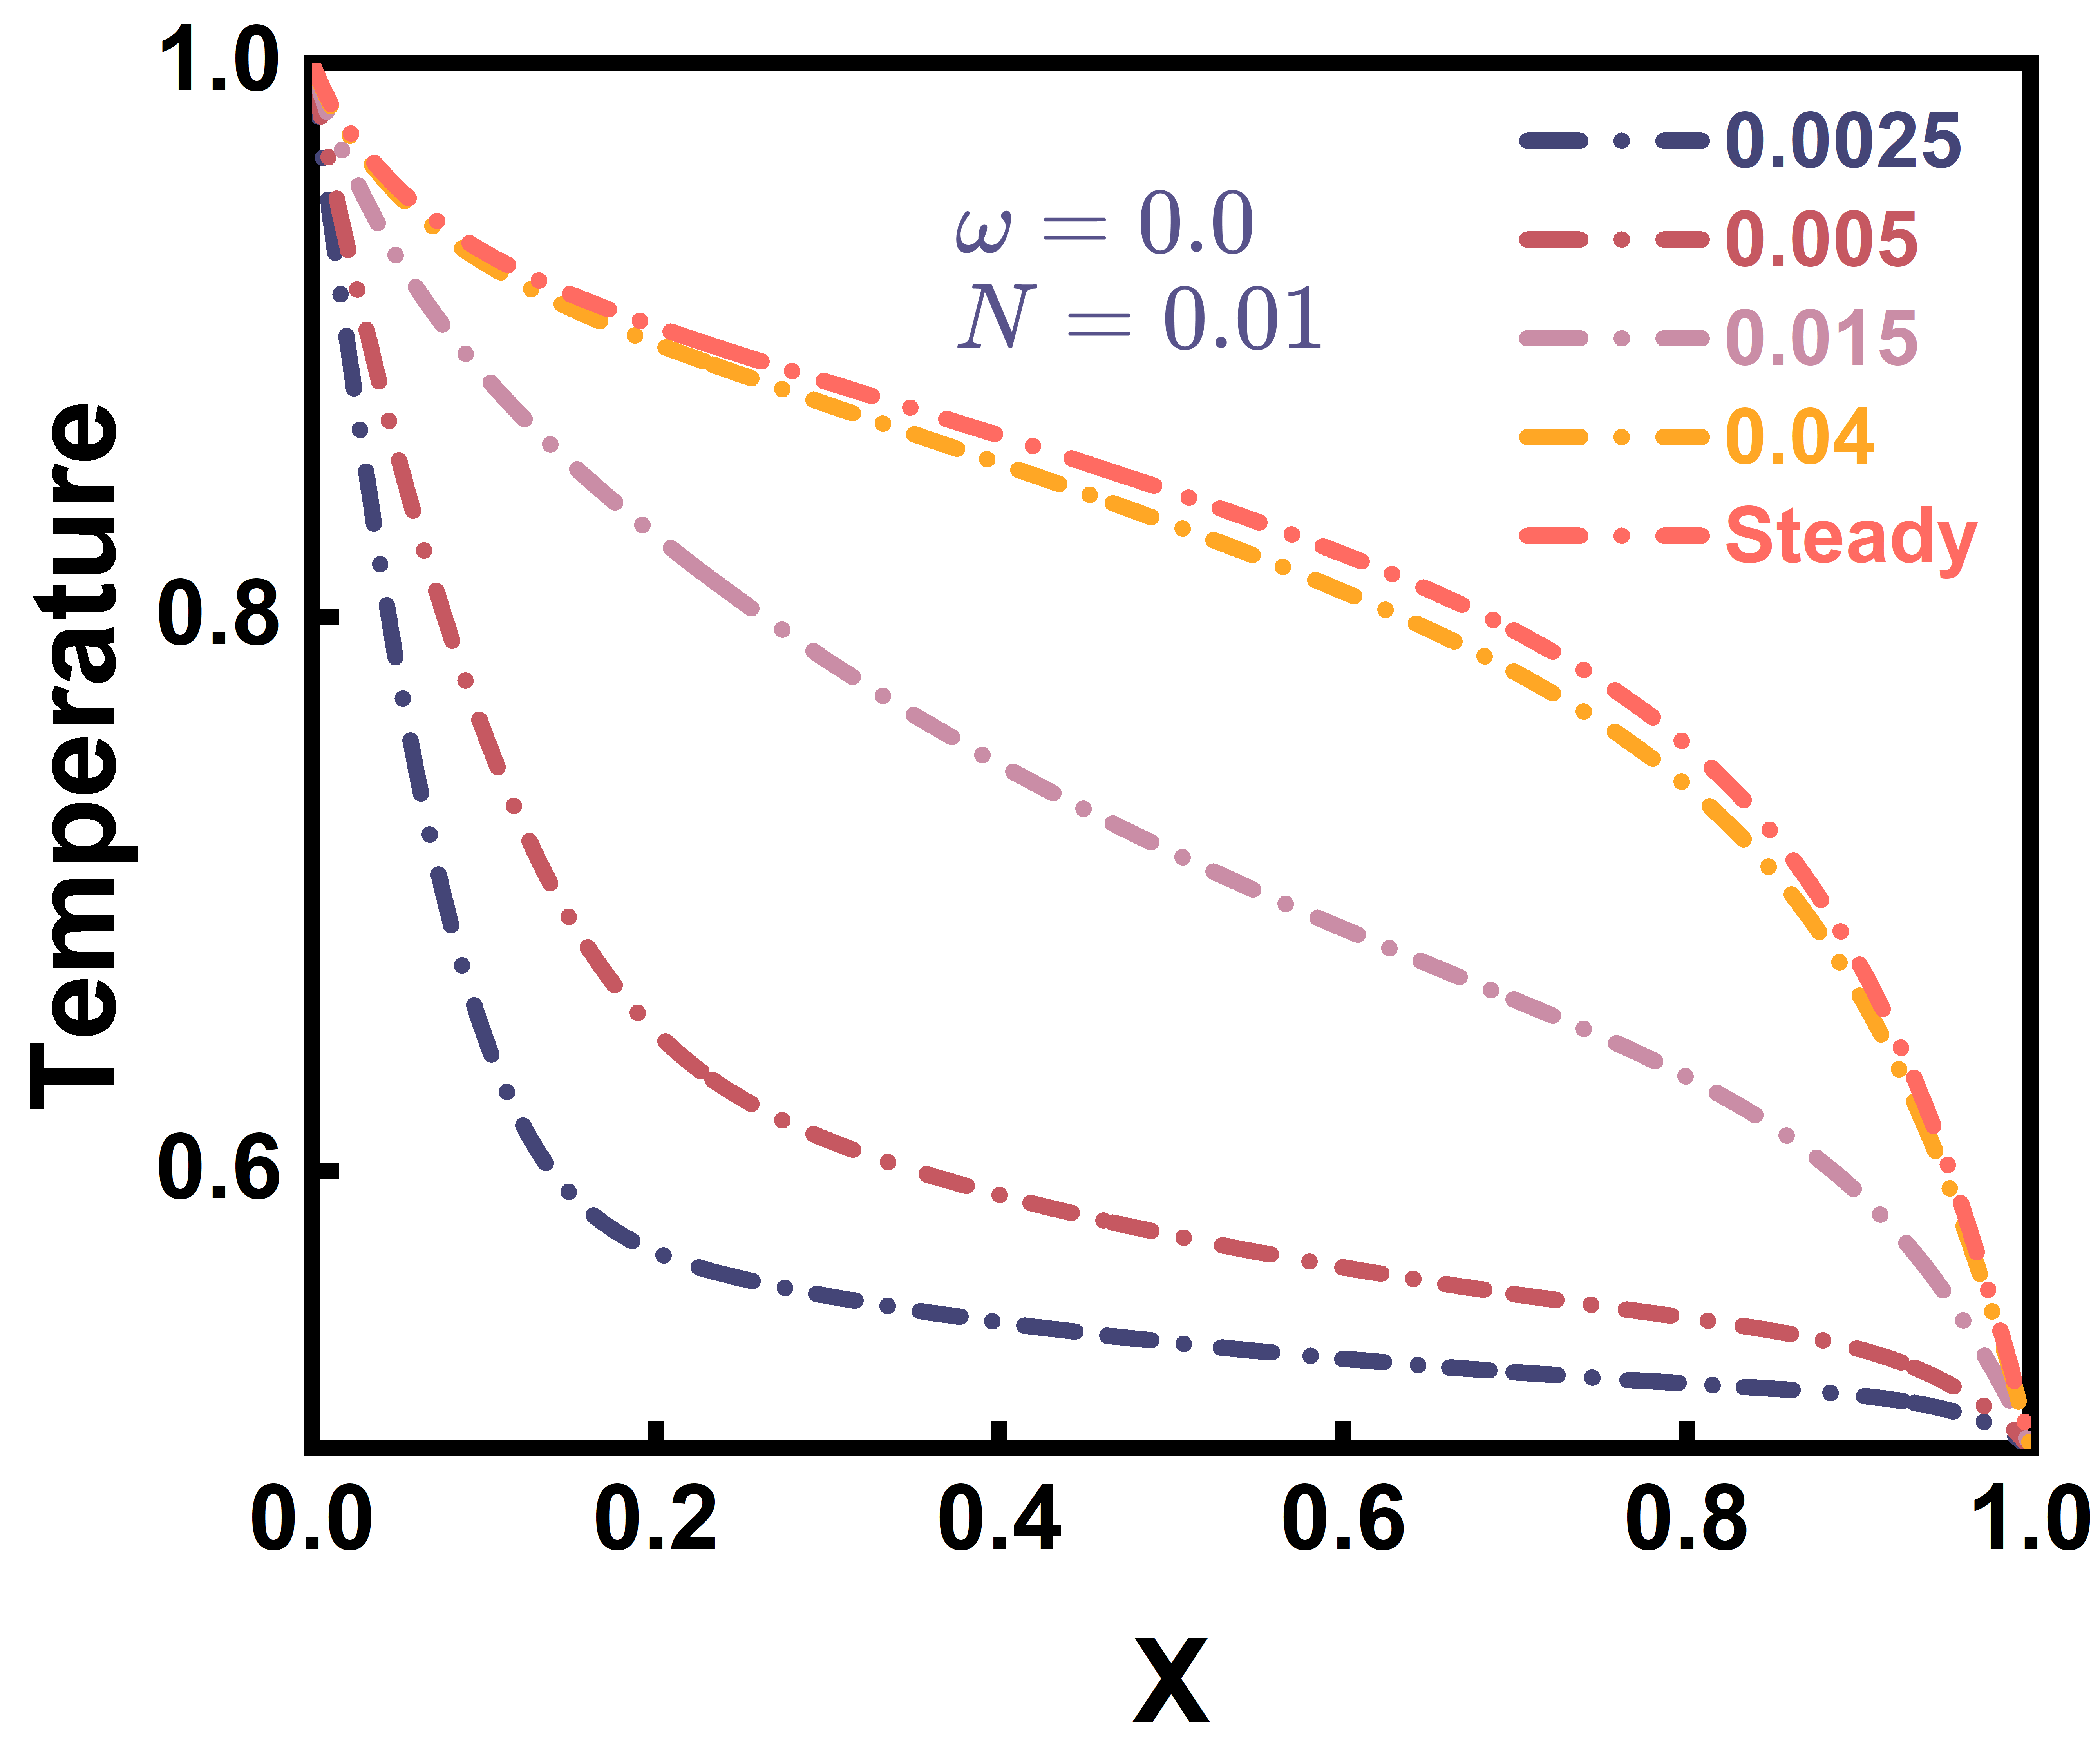
\includegraphics[width=\textwidth]{2A.png}
\caption{}
\end{subfigure}
\hfill
\begin{subfigure}[b]{\figwidth}
\centering
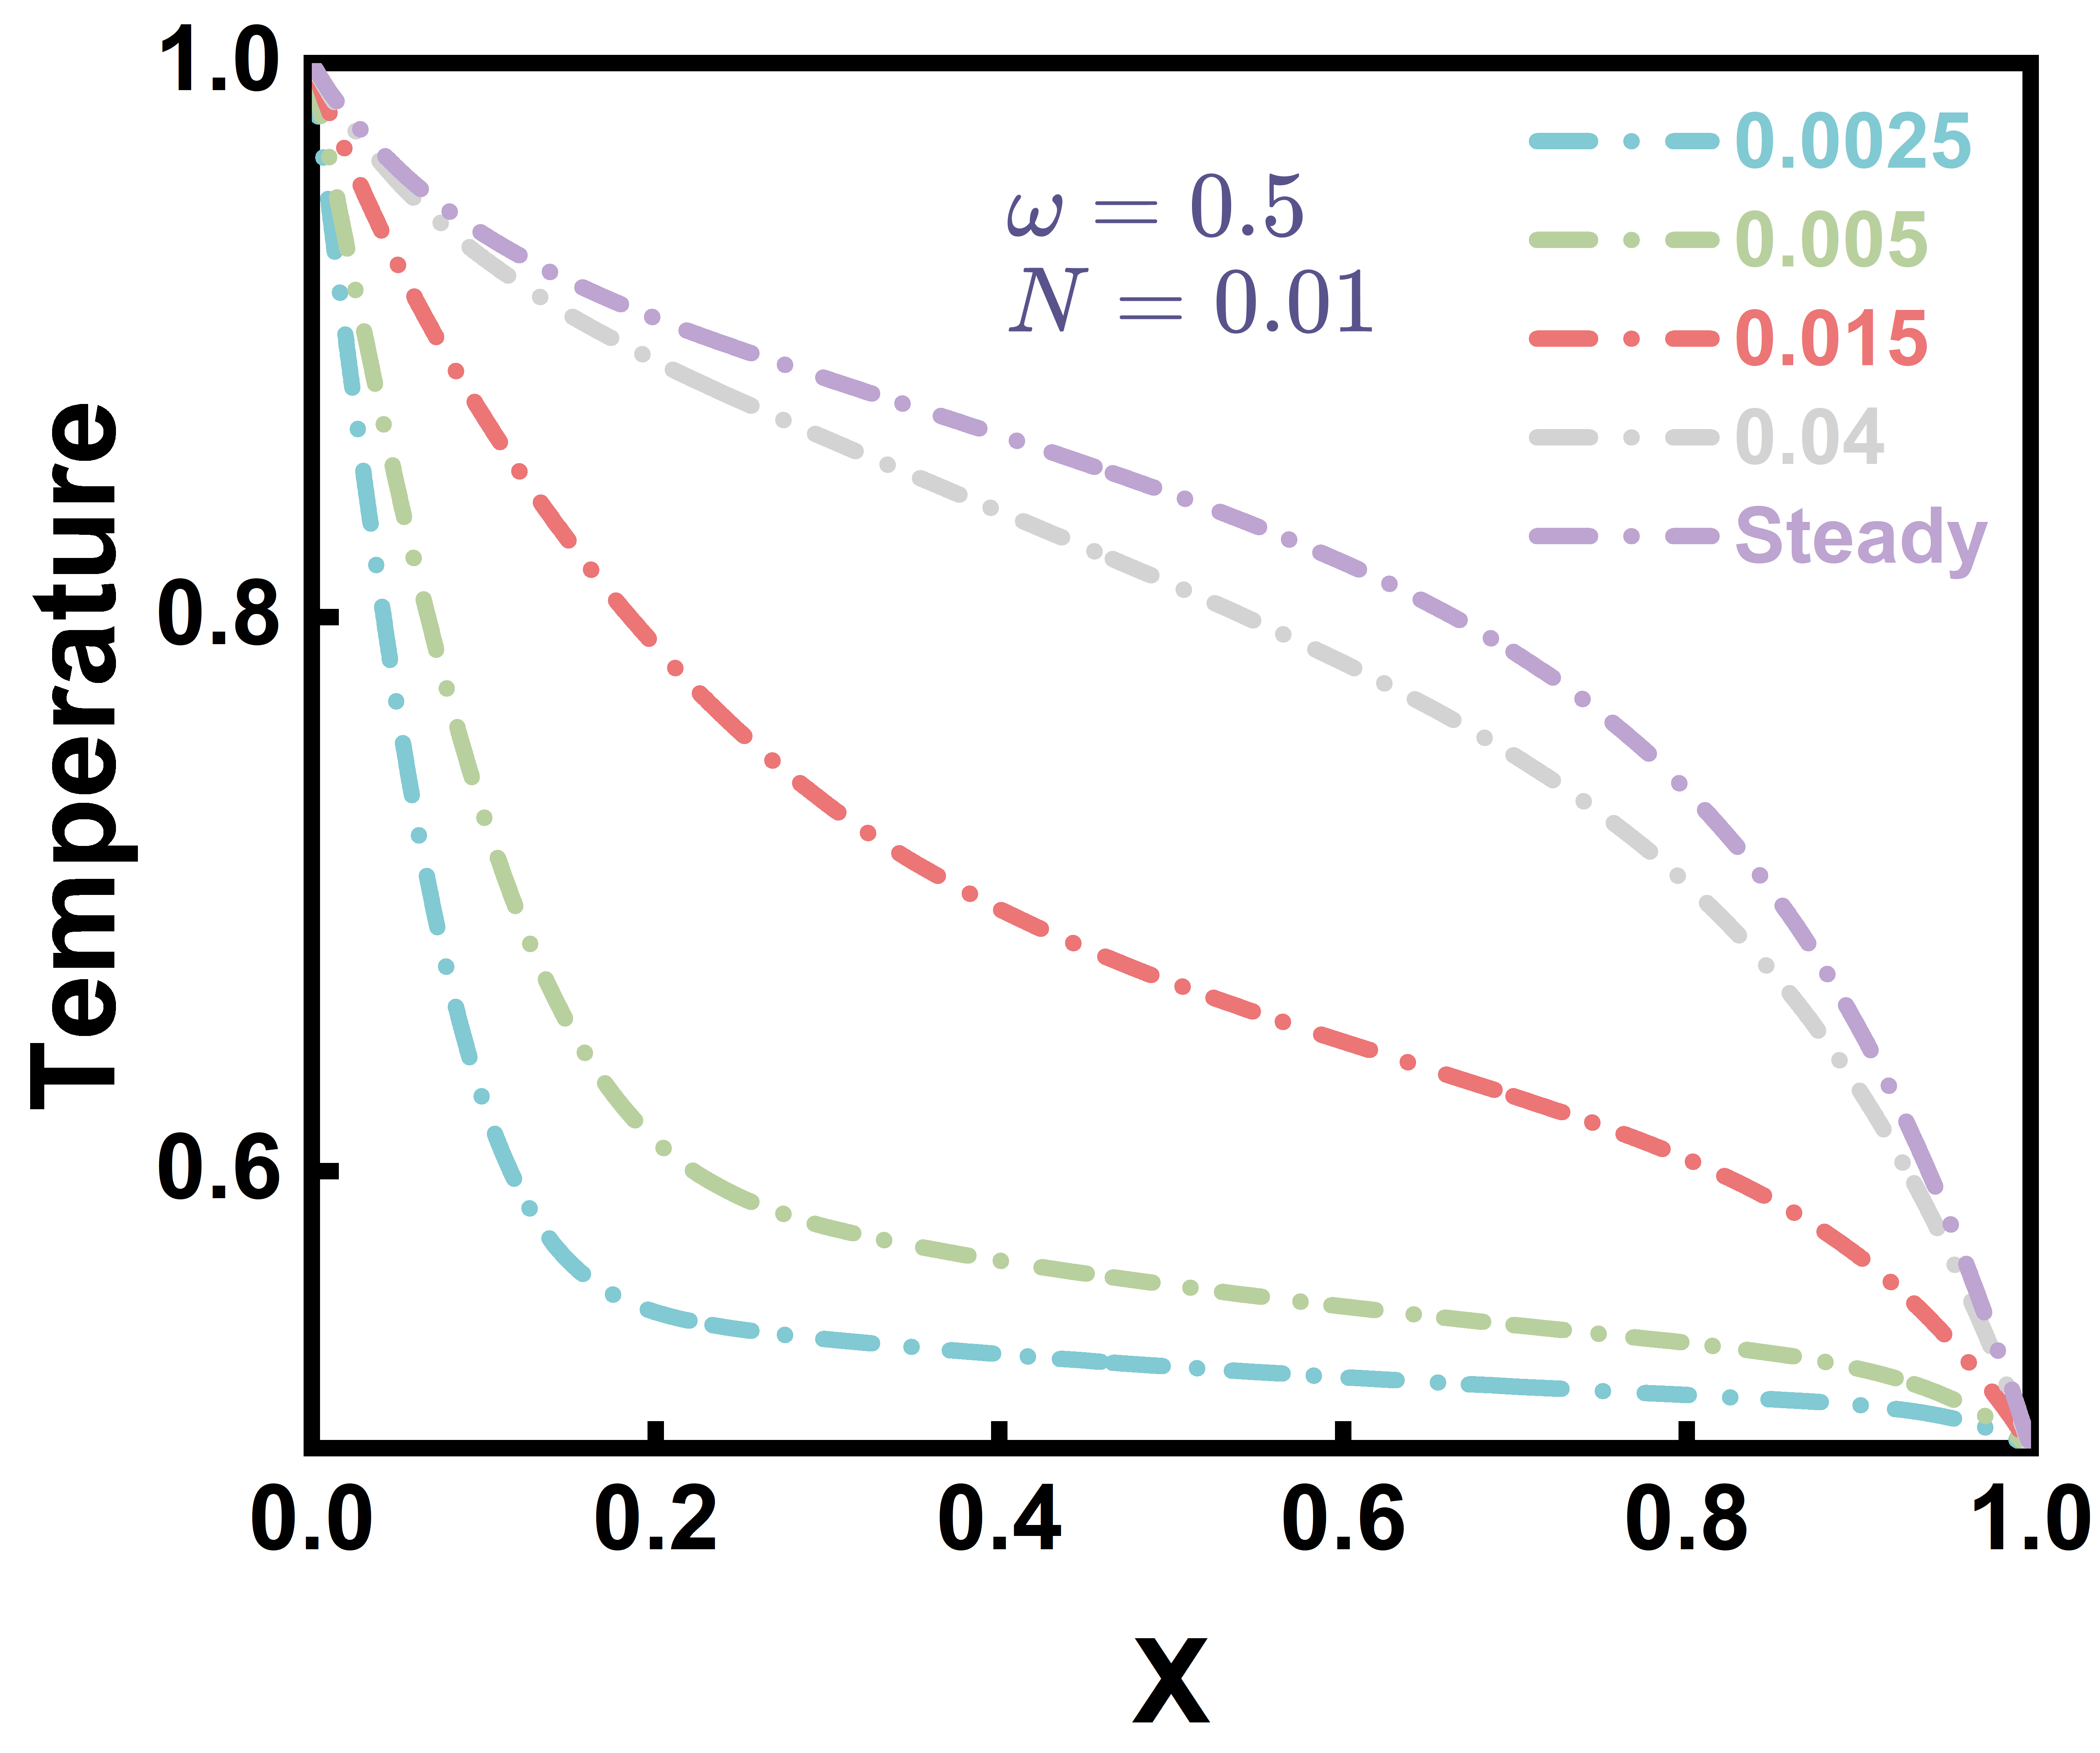
\includegraphics[width=\textwidth]{2B.png}
\caption{}
\end{subfigure}
\hfill
\begin{subfigure}[b]{\figwidth}
\centering
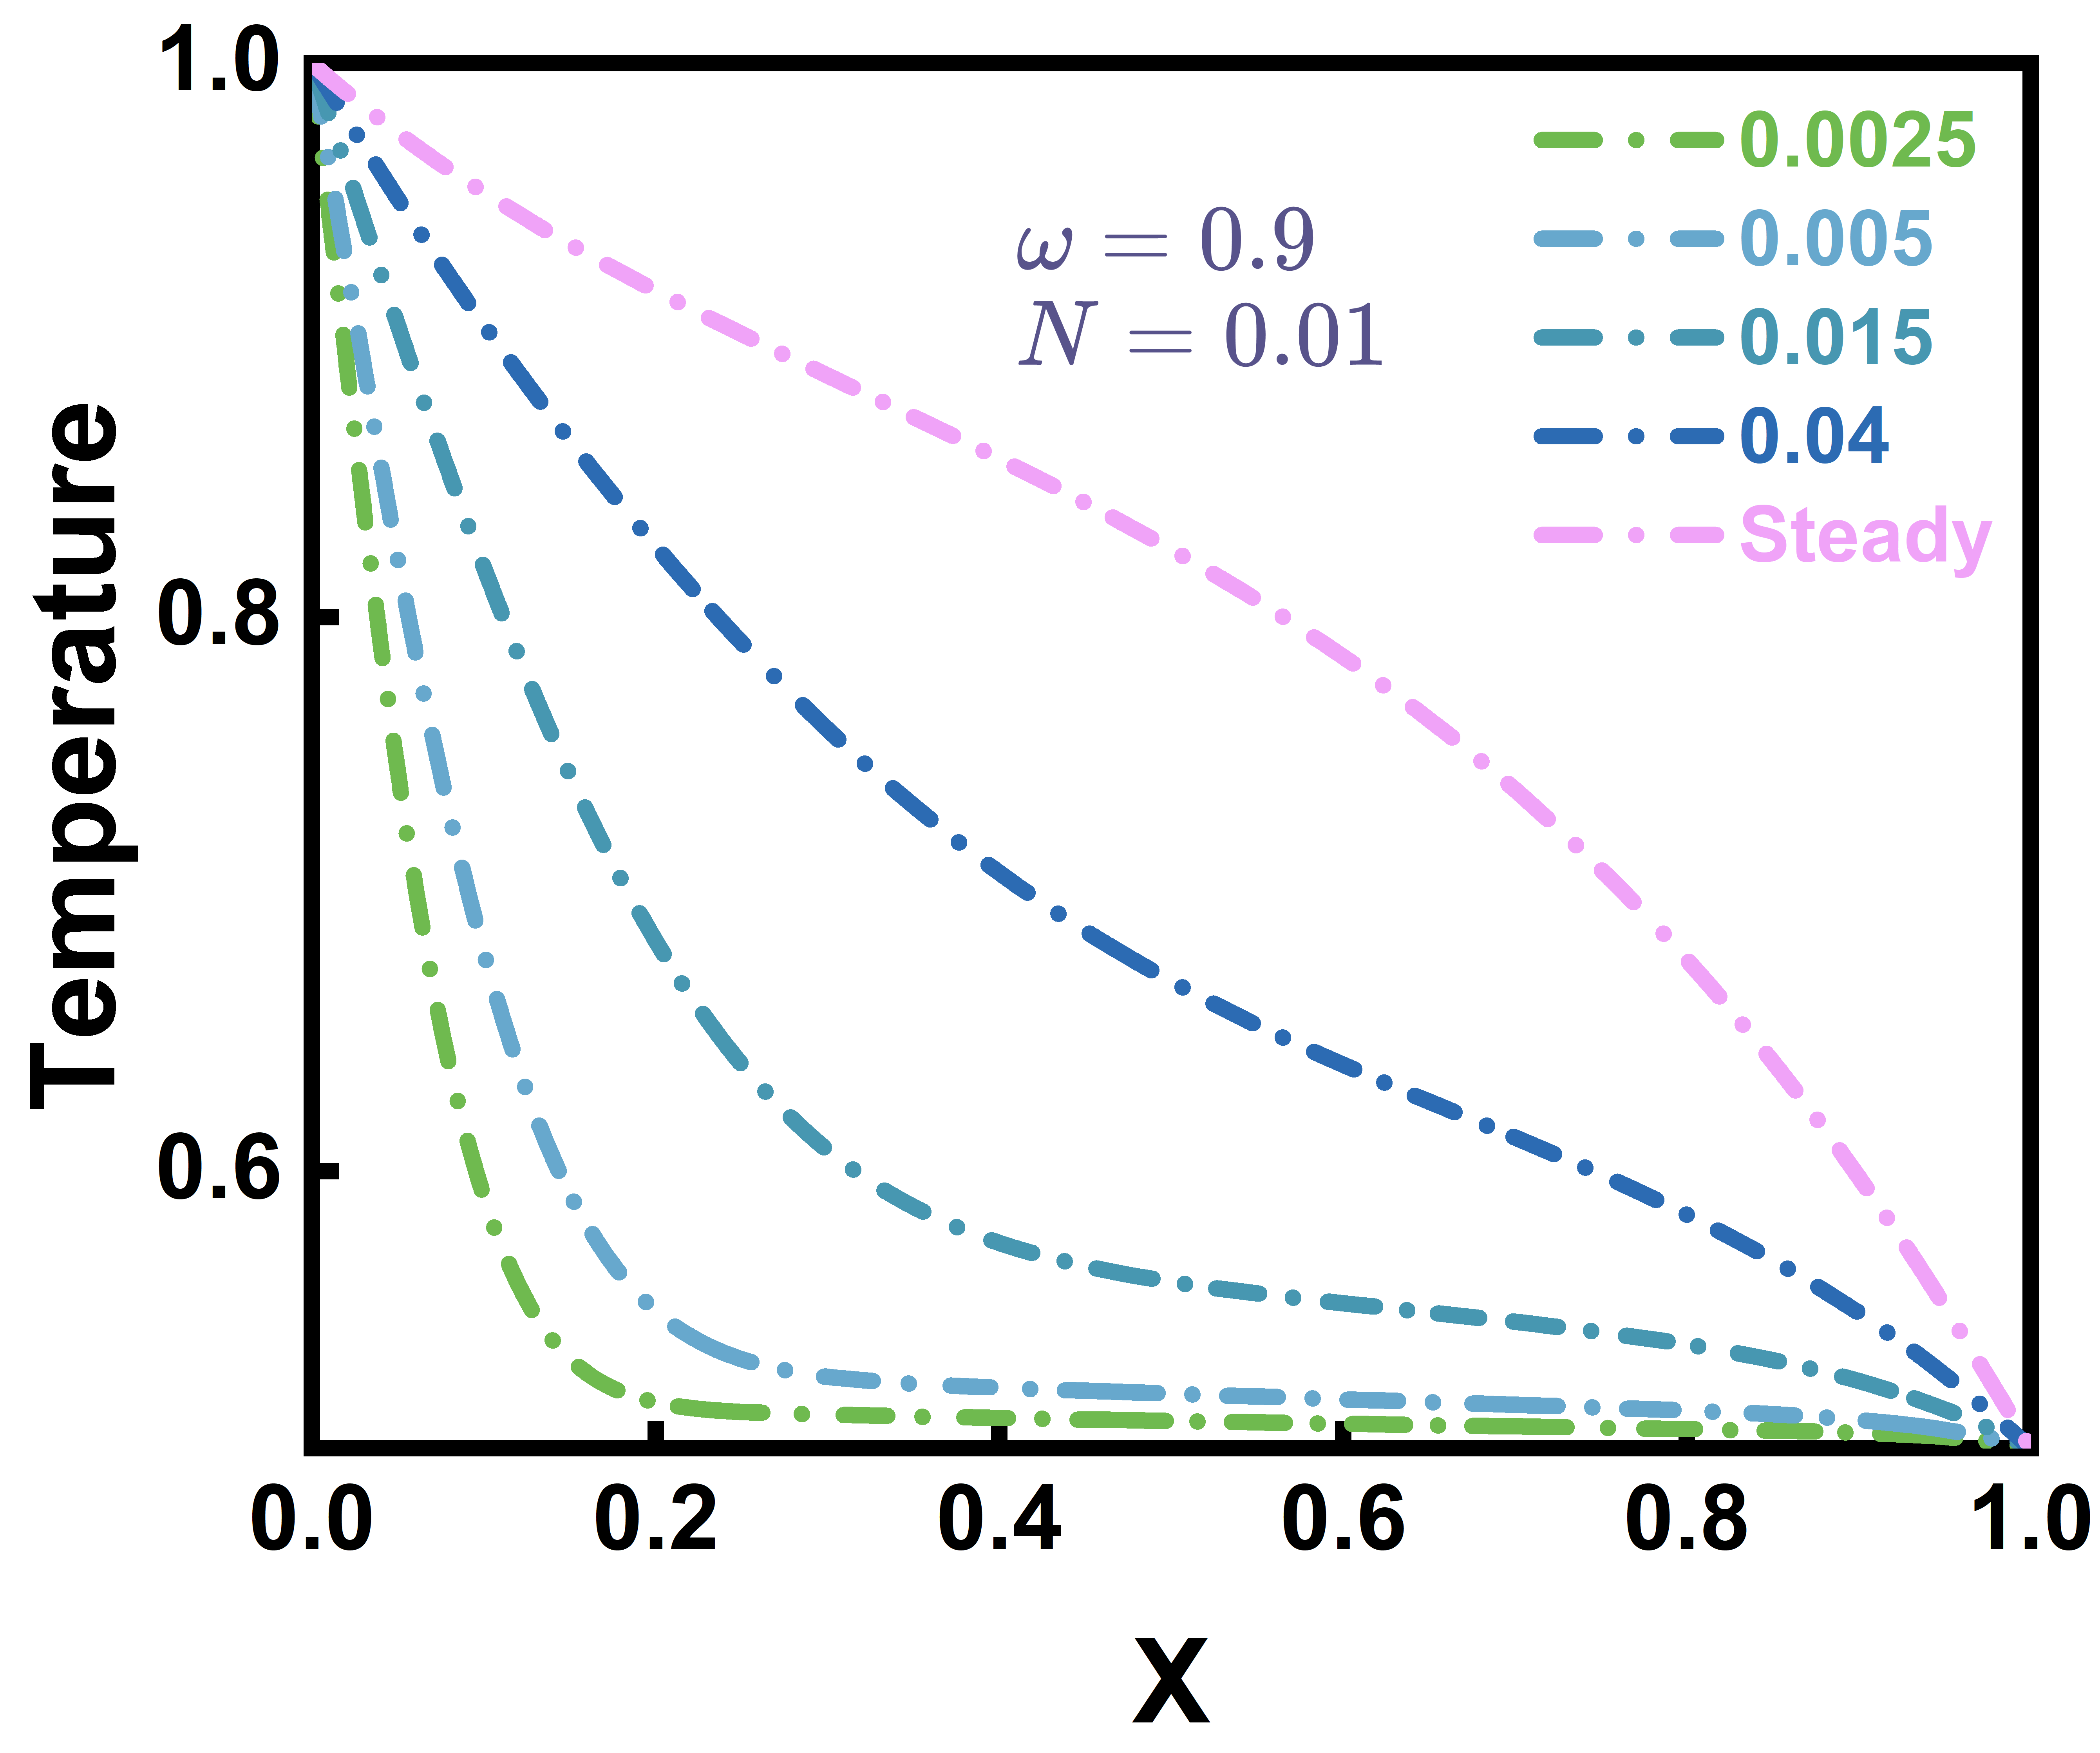
\includegraphics[width=\textwidth]{2C.png}
\caption{}
\end{subfigure}
\caption{Transient dimensionless temperature profiles in a one-dimensional participating slab at $N=0.01$. The scattering albedo is (a) $\omega=0$, (b) $\omega=0.5$,(c) $\omega=0.9$.}
\label{fig2}
\end{figure}

Figure~\ref{fig2} shows the transient temperature profiles at $N=0.01$. The profile was strongly nonlinear at $\omega=0$, and the interior temperature rose rapidly after heating began. Increasing $\omega$ to $0.5$ and $0.9$ lowered the temperature throughout the slab. It also increased the time required to approach steady state. The temperature remained nonlinear while the medium retained a non-zero absorbing component.

\begin{figure}[H]
\centering
\begin{subfigure}[b]{\figwidth}
\centering
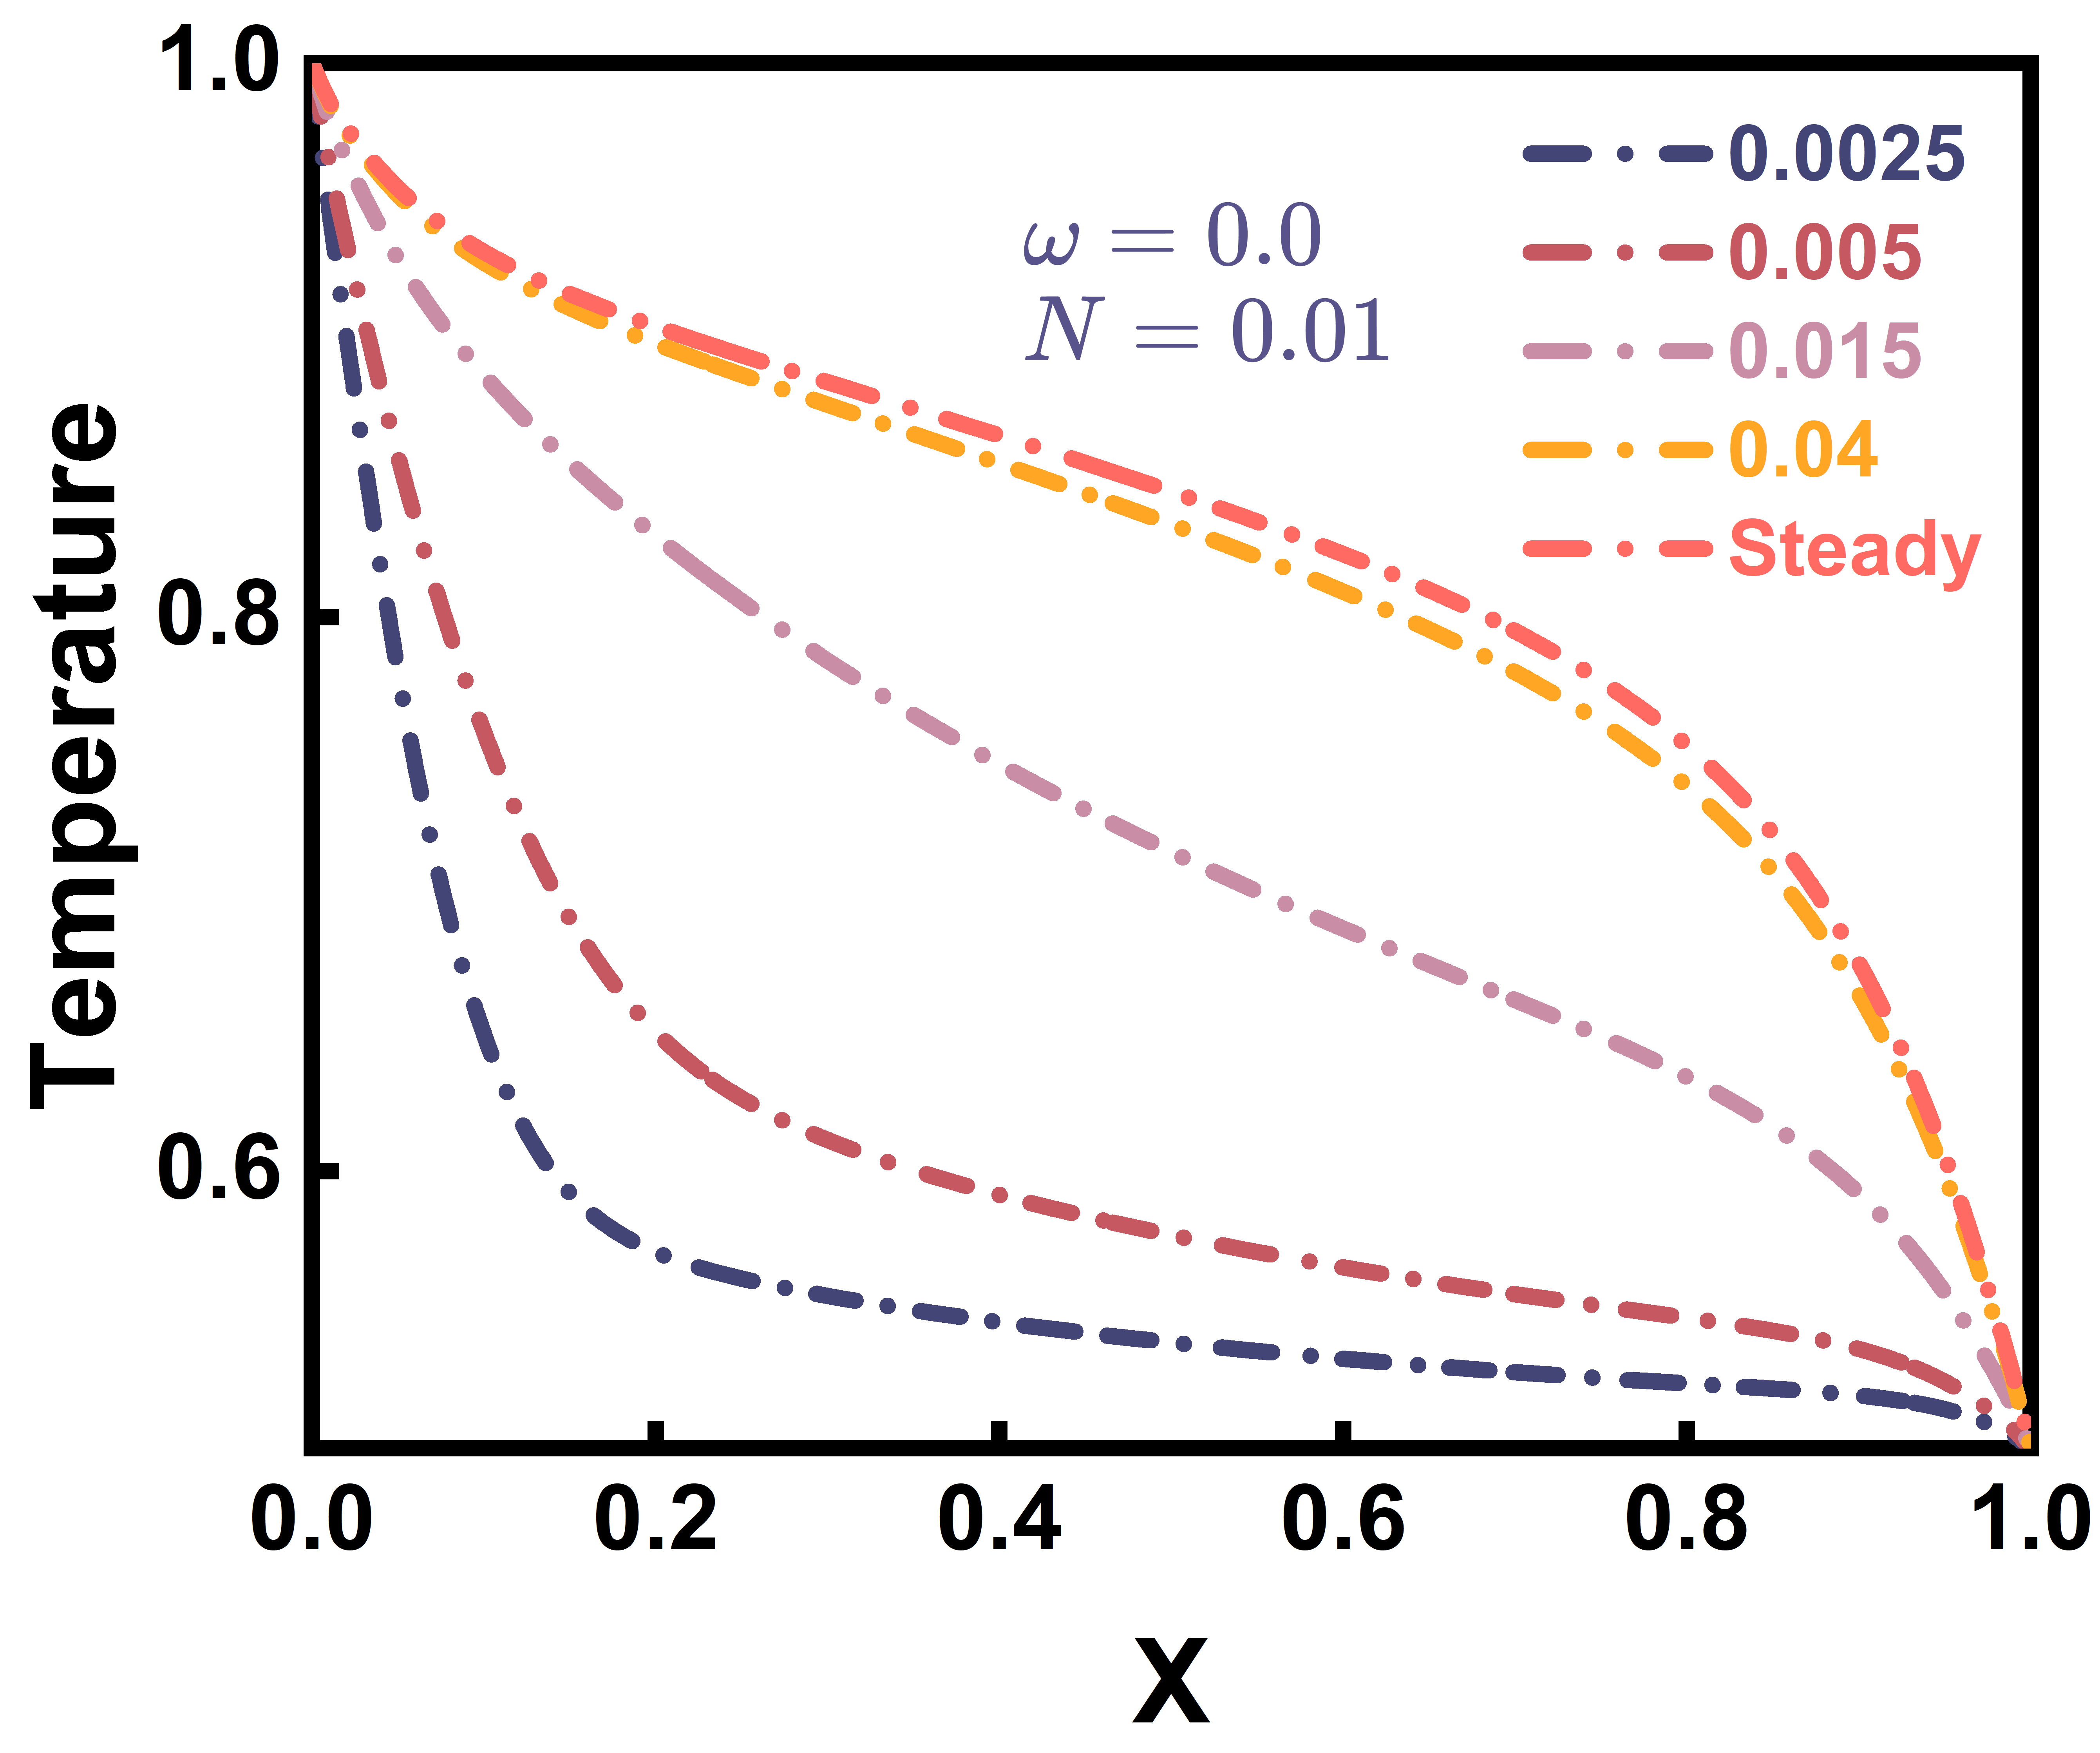
\includegraphics[width=\textwidth]{3A.png}
\caption{}
\end{subfigure}
\hfill
\begin{subfigure}[b]{\figwidth}
\centering
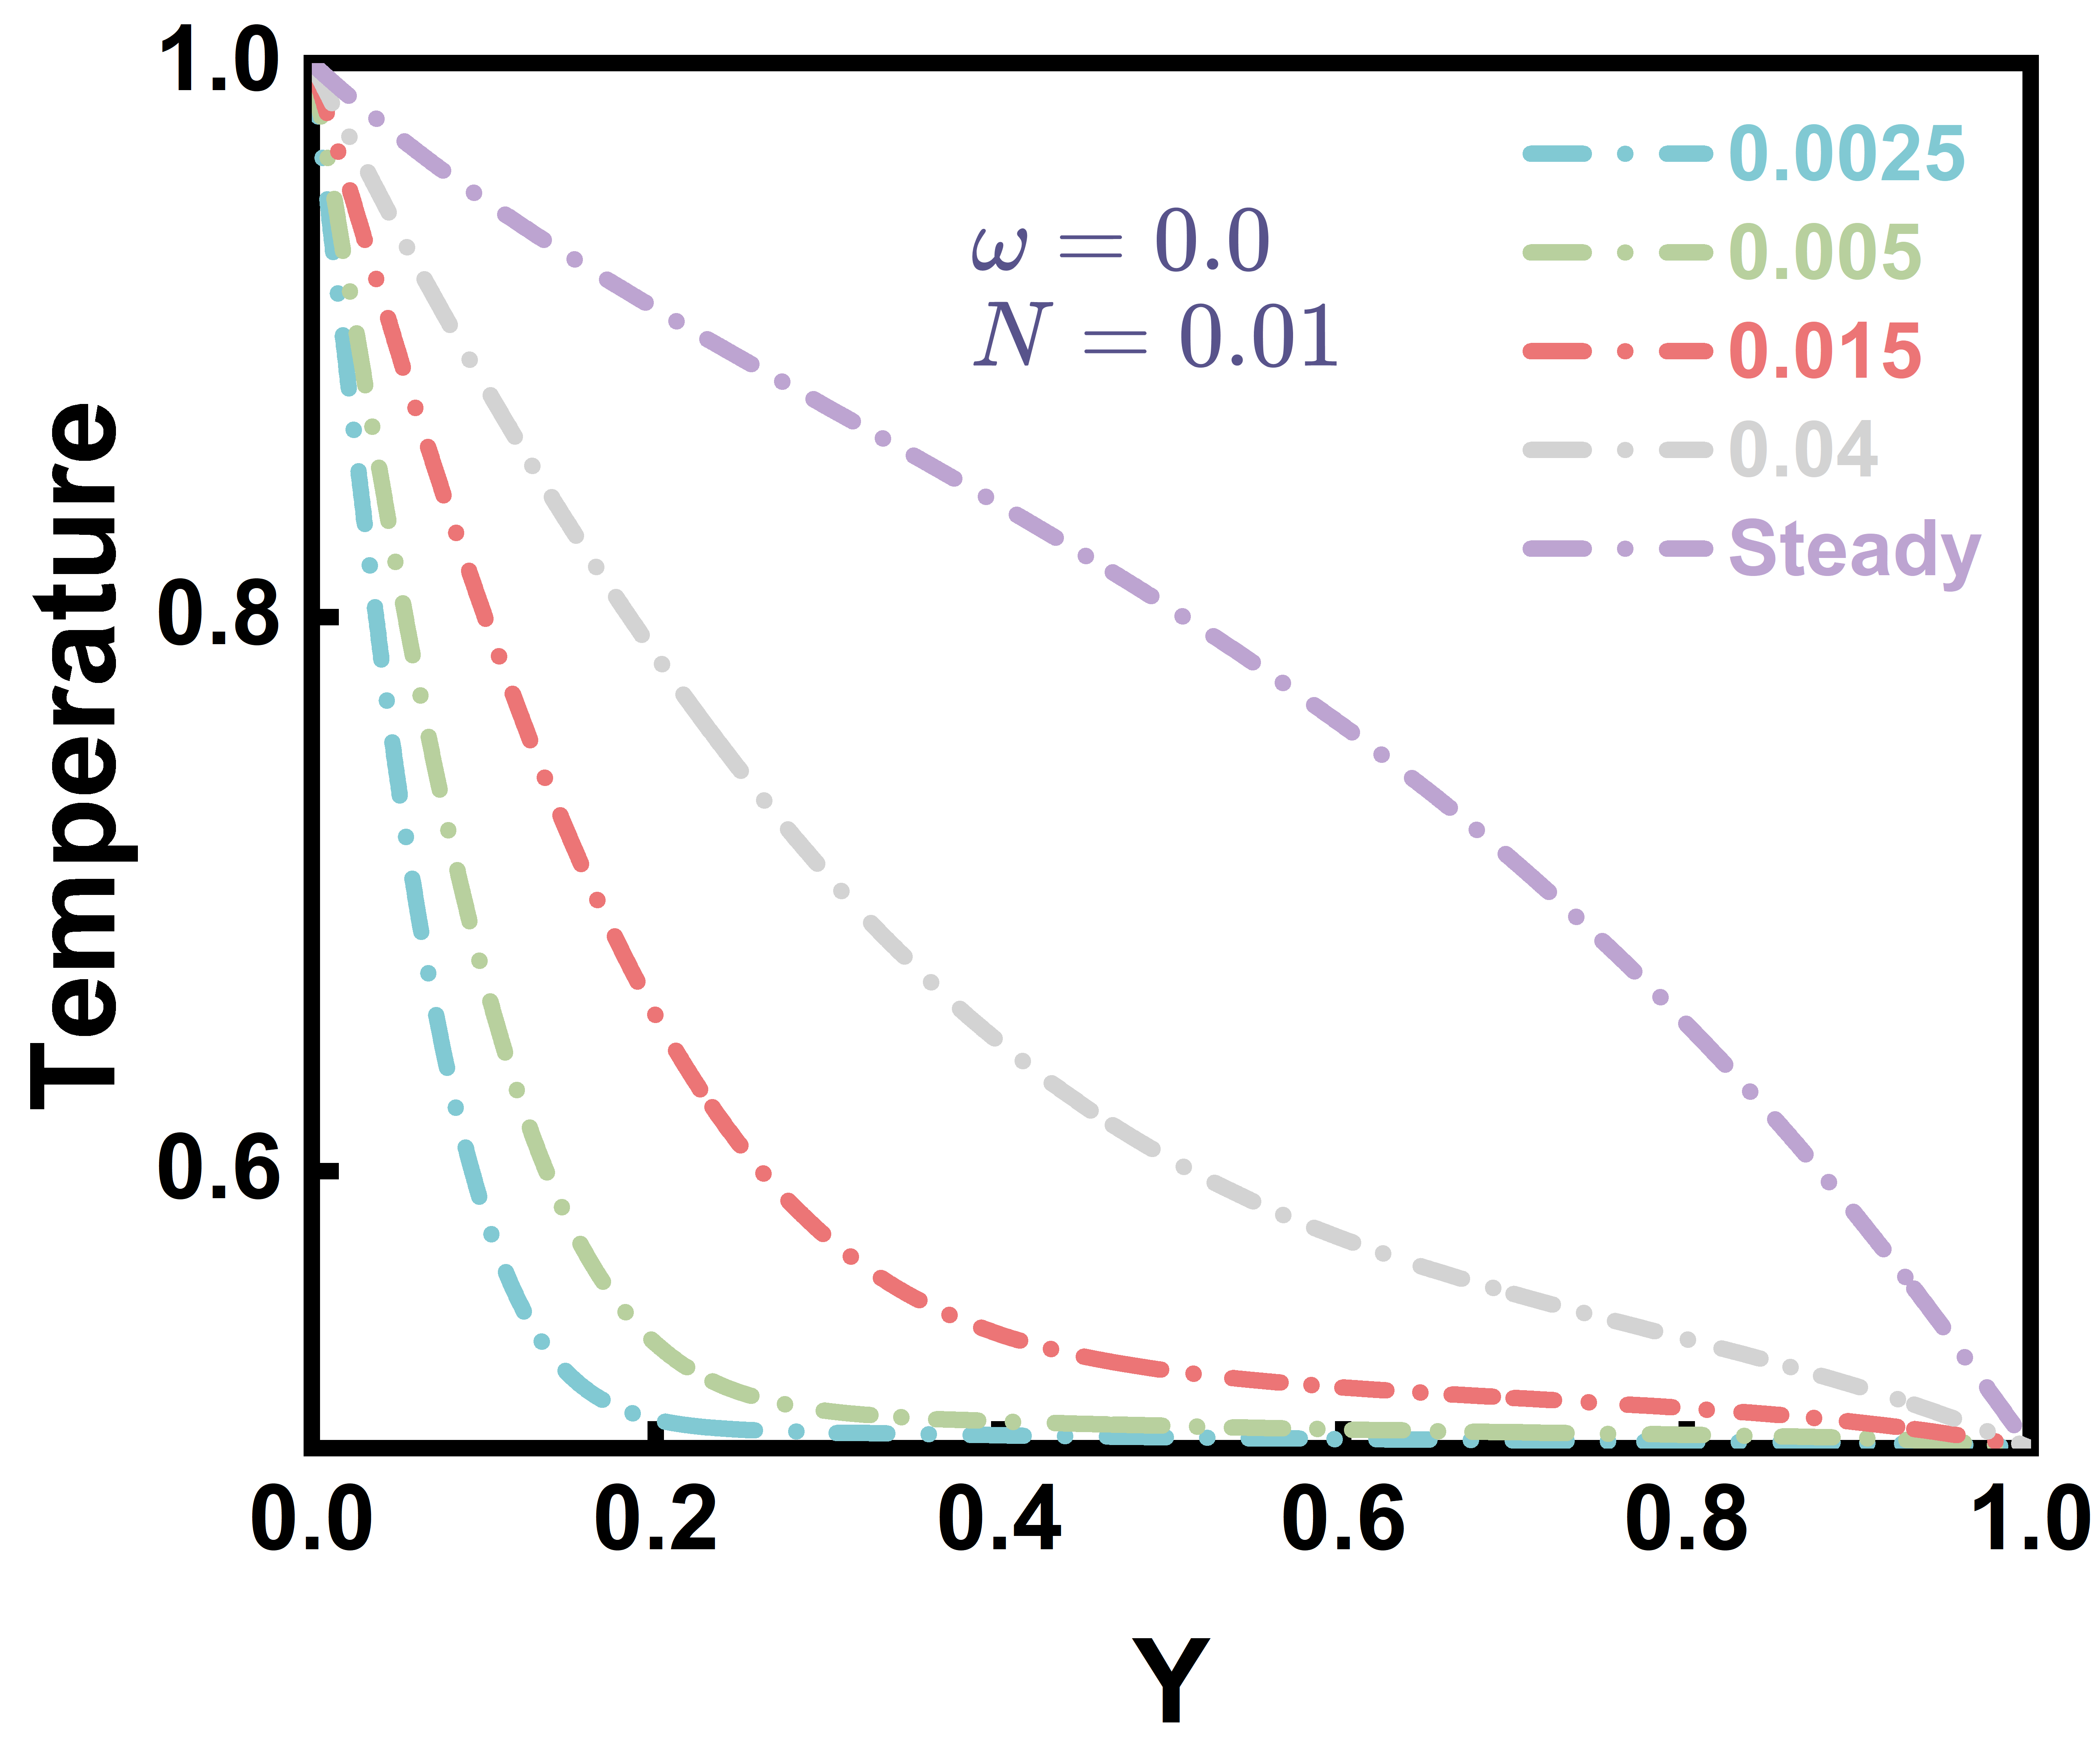
\includegraphics[width=\textwidth]{3B.png}
\caption{}
\end{subfigure}
\hfill
\begin{subfigure}[b]{\figwidth}
\centering
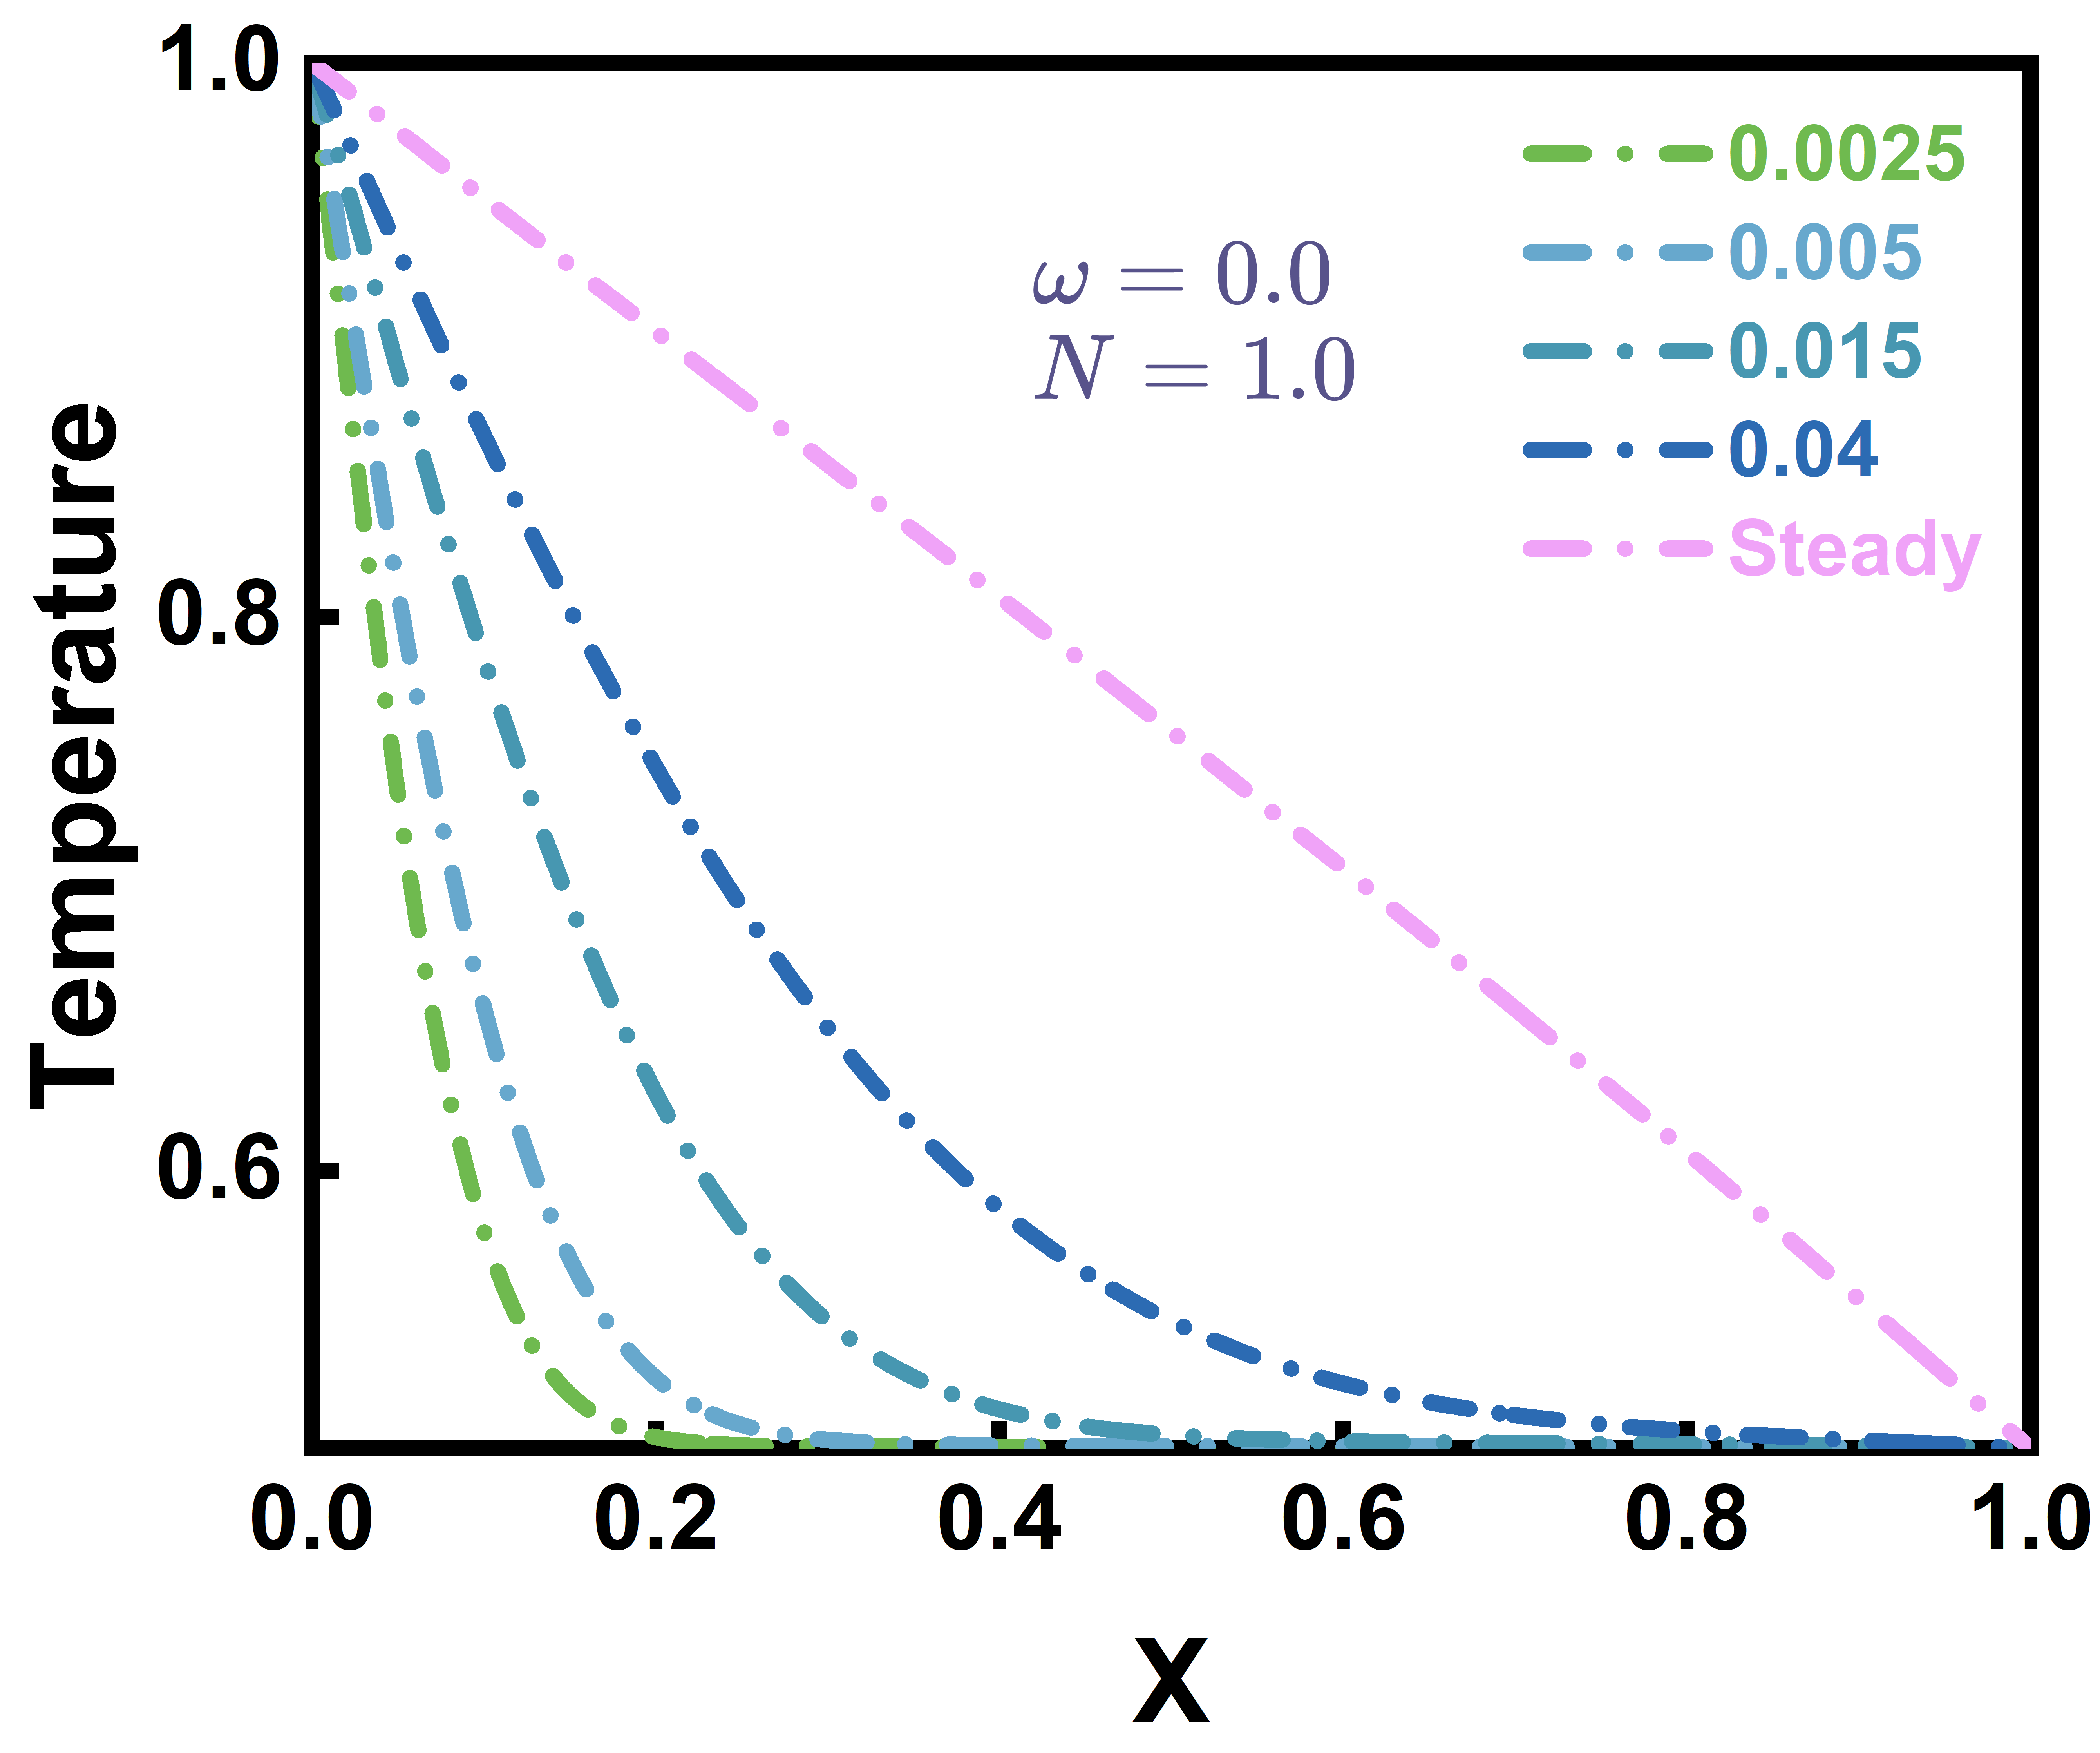
\includegraphics[width=\textwidth]{3C.png}
\caption{}
\end{subfigure}
\caption{Transient dimensionless temperature profiles in a one-dimensional participating slab at $\omega=0$. The conduction--radiation parameter is (a) $N=0.01$, (b) $N=0.10$,(c) $N=1.00$.}
\label{fig3}
\end{figure}

Figure~\ref{fig3} compares transient temperature profiles for different values of $N$. At $N=0.01$, the slab heated rapidly and retained a strongly nonlinear steady-state profile. The curves at $N=0.10$ lay between the radiation-dominated and conduction-dominated limits. At $N=1.00$, early heating remained concentrated near the hot wall, and the steady-state profile approached a linear distribution. Increasing $N$ therefore lowered the slab temperature and delayed thermal penetration towards the cold wall.

Figure~\ref{fig4} reports the flux profiles at $\zeta=0.005$ for $N=0.10$, $T_E=0.1$, and unit optical thickness. Conductive flux was obtained from the temperature gradient, whereas radiative flux was calculated from the first angular moment of intensity. Both components contributed at $\omega=0$, while the radiative component decreased as $\omega$ increased. At $\omega=1.0$, the volumetric radiative source vanished and conduction governed the thermal response. The decomposed fluxes agreed with the collapsed-dimension benchmark of Talukdar and Mishra~\cite{Talukdar2001} for the same configuration.

\begin{figure}[H]
\centering
\begin{subfigure}[b]{\figwidth}
\centering
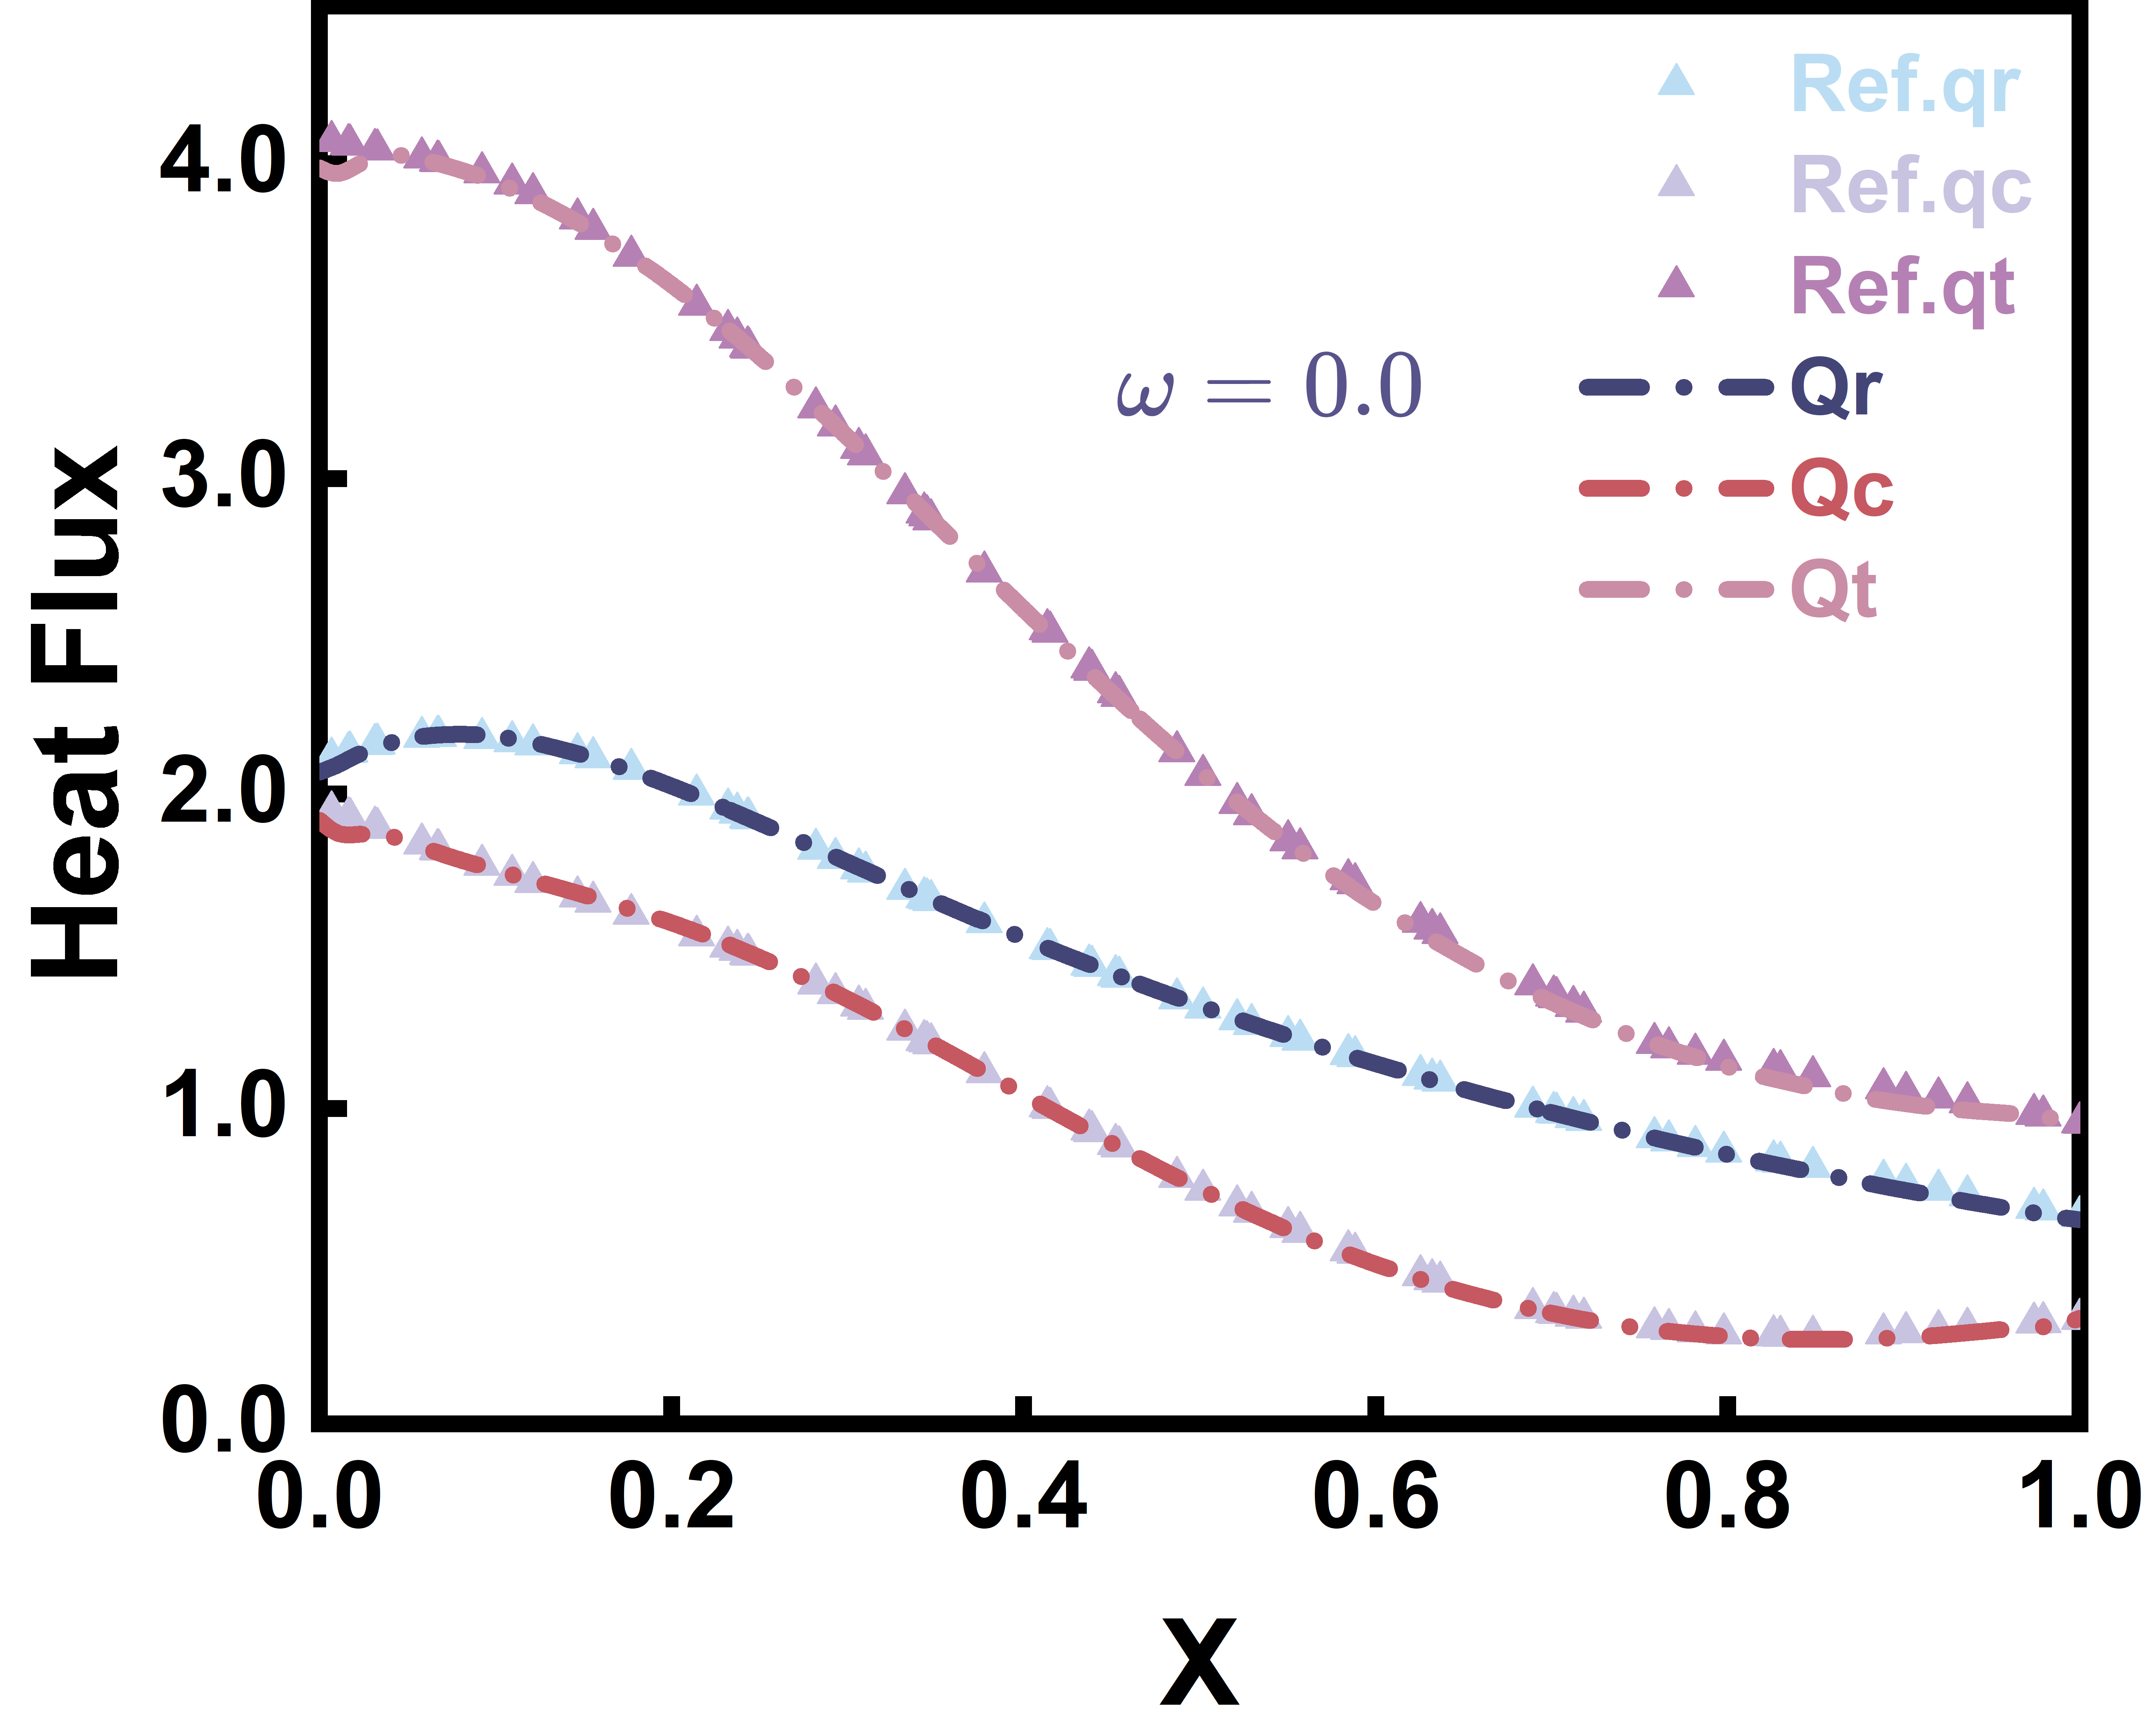
\includegraphics[width=\textwidth]{4A.png}
\caption{}
\end{subfigure}
\hfill
\begin{subfigure}[b]{\figwidth}
\centering
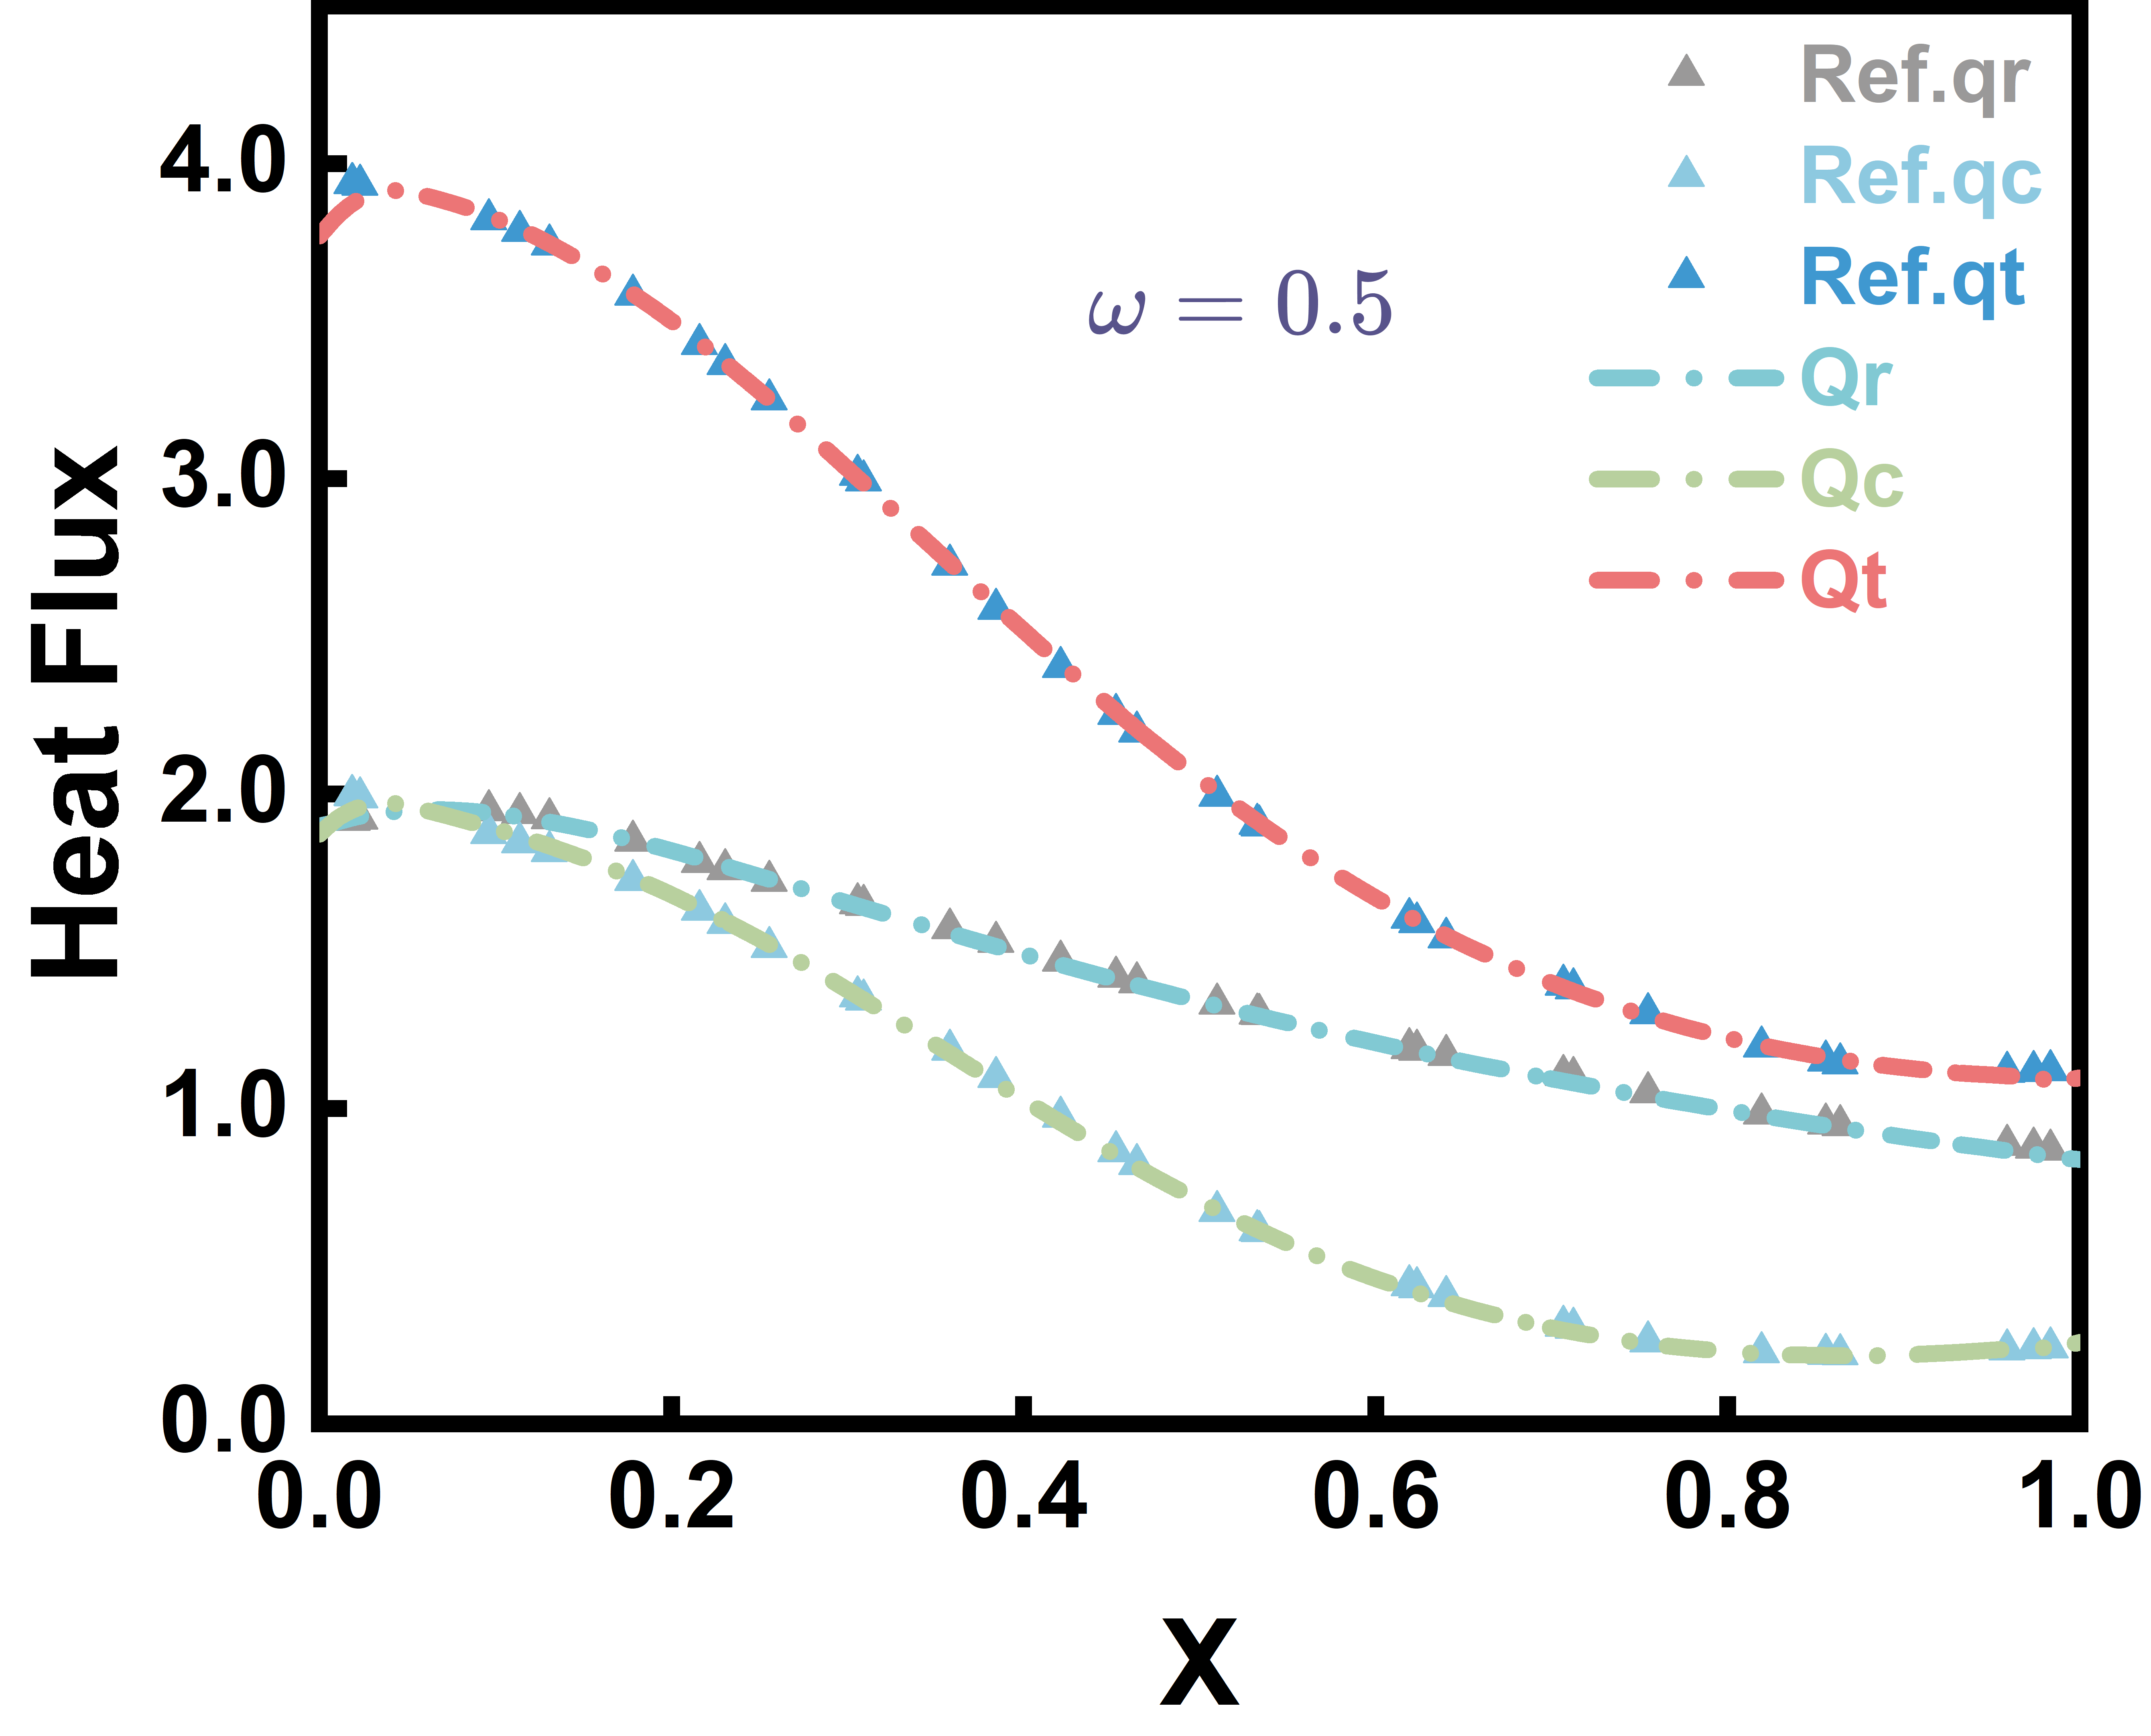
\includegraphics[width=\textwidth]{4B.png}
\caption{}
\end{subfigure}
\hfill
\begin{subfigure}[b]{\figwidth}
\centering
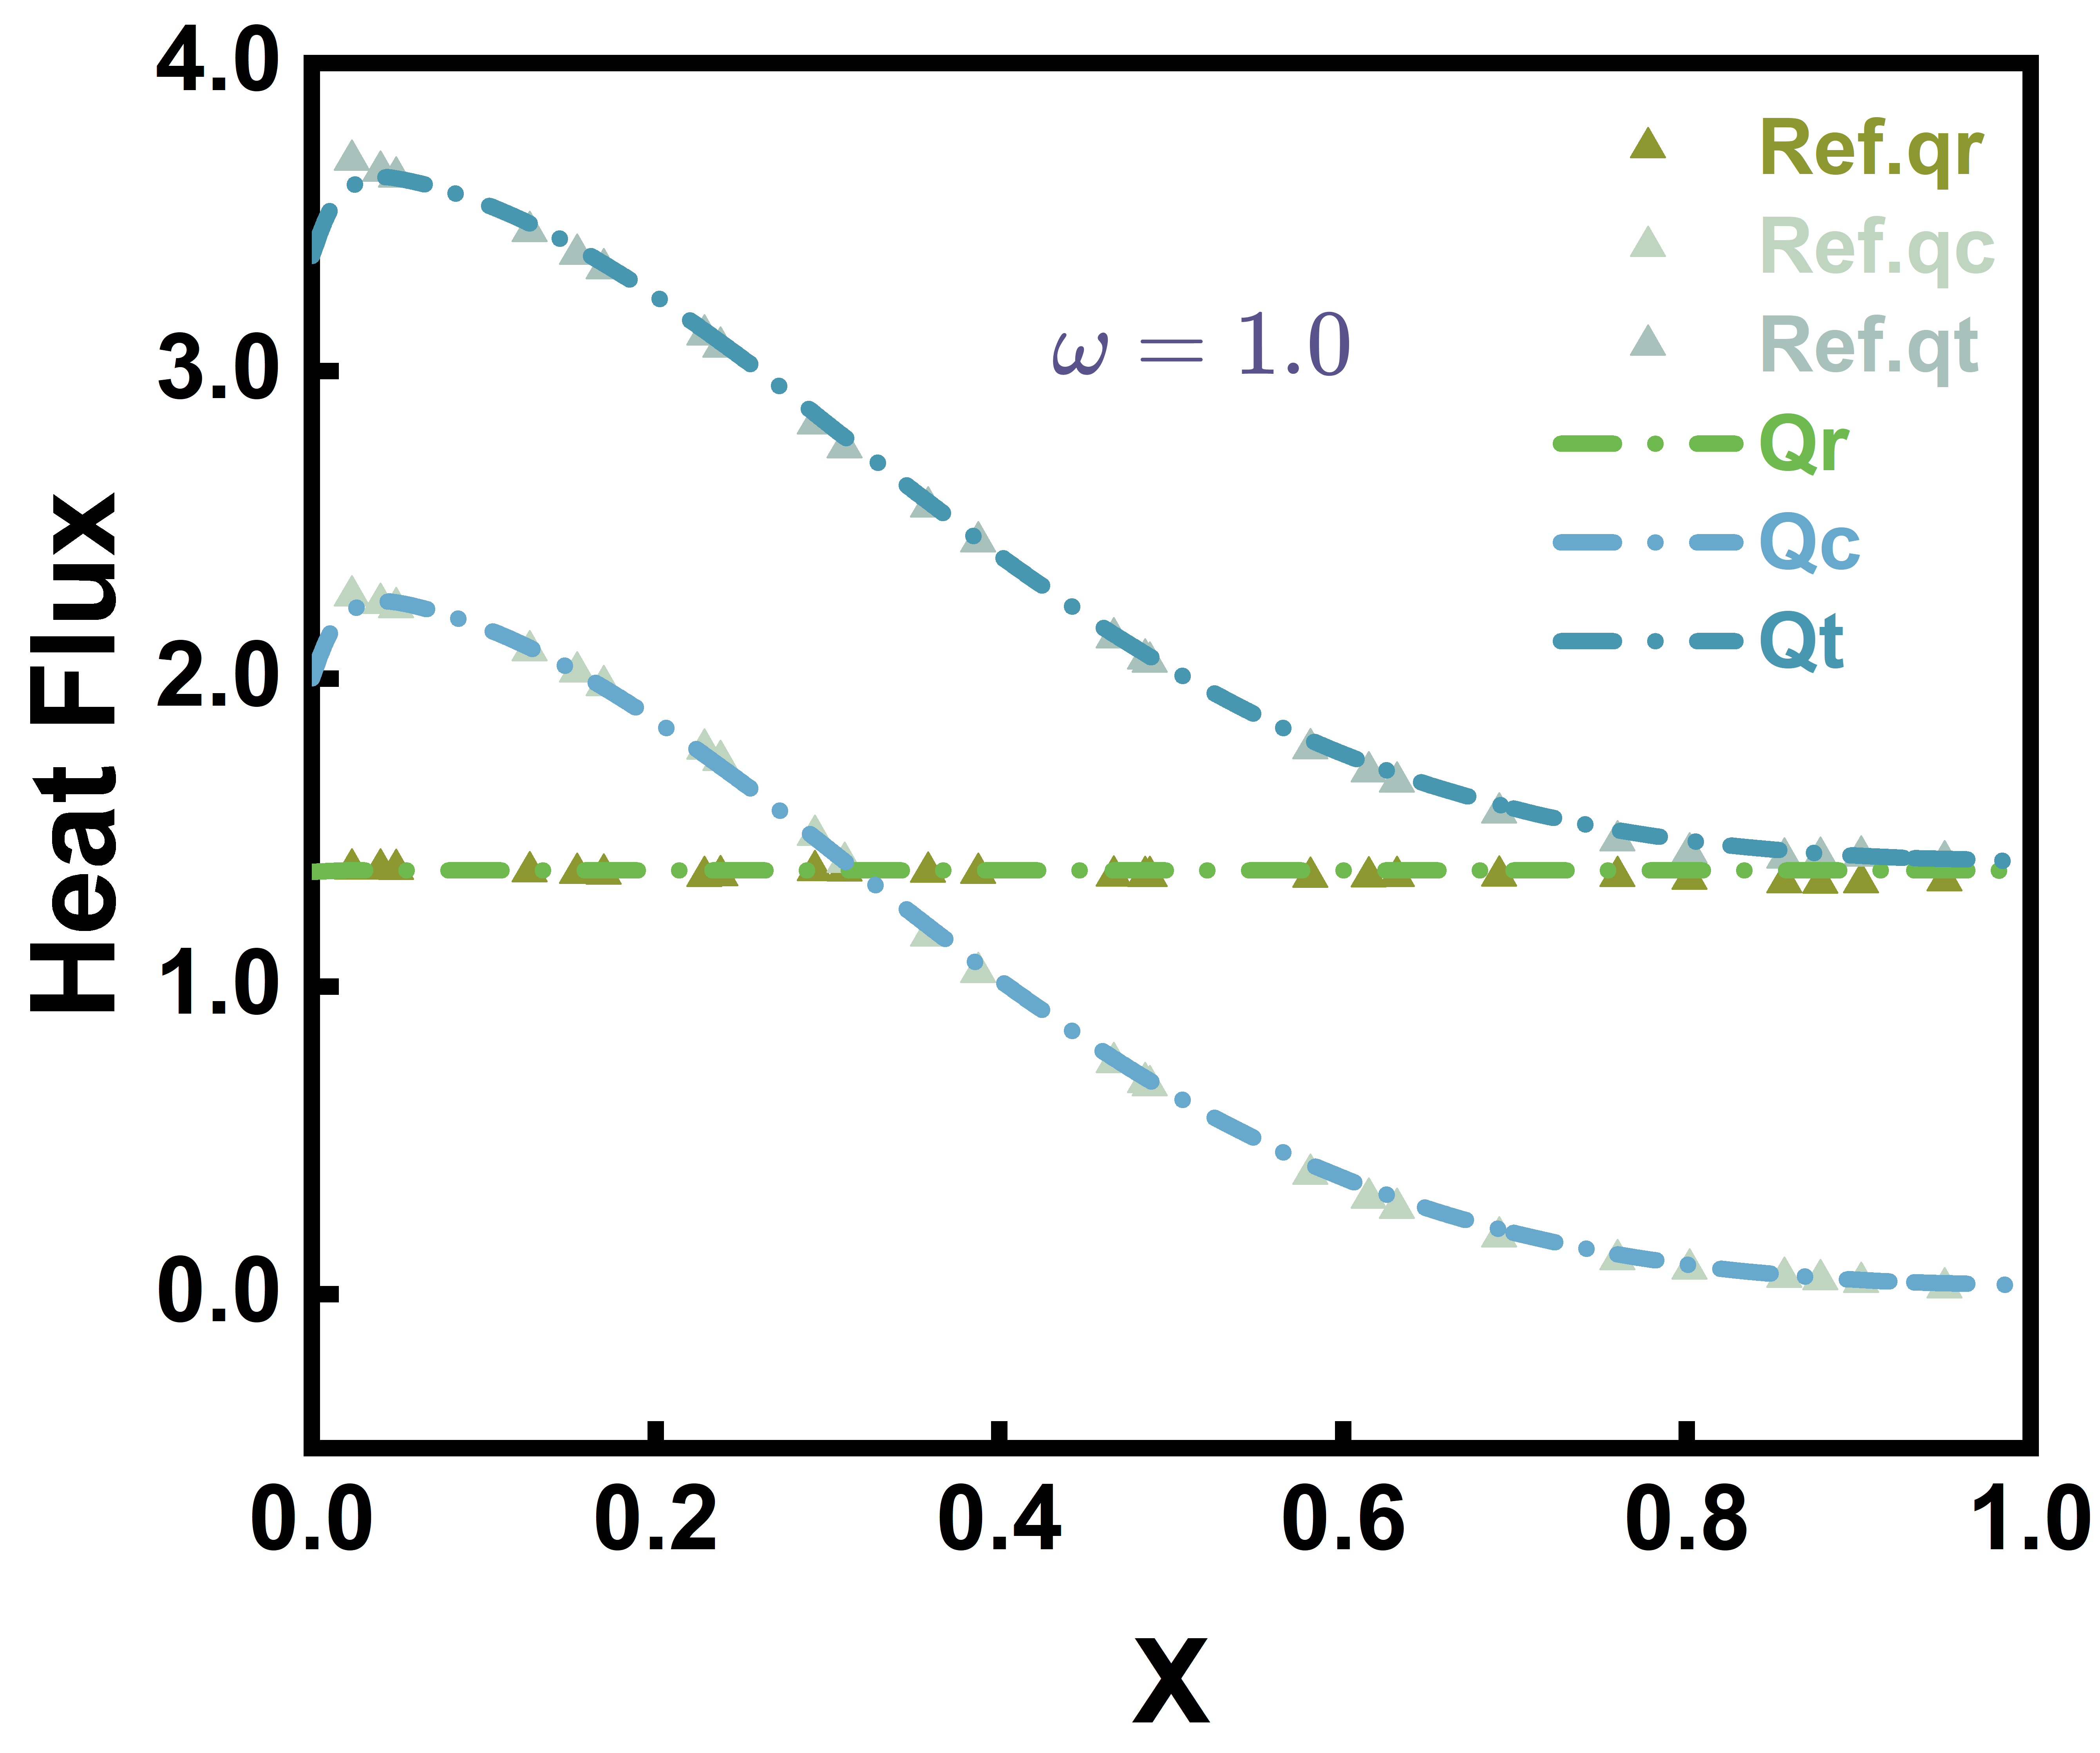
\includegraphics[width=\textwidth]{4C.png}
\caption{}
\end{subfigure}
\caption{Conductive, radiative, and total heat-flux profiles in the one-dimensional participating slab. The profiles are evaluated at $\zeta=0.005$ with $N=0.10$ , $T_E=0.1$. The scattering albedo is (a) $\omega=0$, (b) $\omega=0.5$,(c) $\omega=1.0$.}
\label{fig4}
\end{figure}

\subsection{2D cases}
\label{subsec:2d_cases}

The two-dimensional domain was a square medium of side length $L$, represented by $0\leq X,Y\leq1$. The square was initially at a uniform temperature $T_0$. At $t\geq0$, the south wall was raised to $T_S$ and held constant. The north, west, and east walls remained at $T_0$. All properties were constant, and the optical thickness was $1.0$ in both coordinate directions.

A uniform $41\times41$ mesh was used after further refinement produced negligible changes in the centreline temperature. The number of azimuthal control volumes was varied to assess angular sensitivity along the vertical centreline. Steady-state temperatures at $Y=0.3$, $0.5$, and $0.7$ were compared with the original benchmark matrix reproduced by Sun and Zhang~\cite{Sun2016} from Wu and Ou~\cite{WuOu1994}, Yuen and Takara~\cite{YuenTakara1988}, and Mondal and Mishra~\cite{MondalMishra2007}. For each value of $N$, the LBM--FVM solution reported by Sun and Zhang is included as a separate reference row, followed by the present DUGKS result. The comparison used $\tau_L=1.0$, $\omega=0$, $T_0=0.5$, and $N=1.0$, $0.1$, and $0.01$. Subsequent tests varied scattering albedo and the conduction--radiation parameter along the same centreline.

\begin{table}[H]
\centering
\scriptsize
\caption{Steady dimensionless temperature $T/T_S$ on the vertical centreline of the two-dimensional square enclosure at $\tau_L=1.0$, $\omega=0$, and $T_0=0.5$. The original comparison data and the LBM--FVM solutions are taken from Sun and Zhang~\cite{Sun2016}; for each $N$, the present DUGKS results obtained using $N_\theta=8$ and $N_\phi=16$ are listed immediately after the LBM--FVM reference.}
\label{tab:square_validation}
\resizebox{\textwidth}{!}{%
\begin{tabular}{@{}c l ccc@{}}
\toprule
$N$ & Investigator/method & $Y=0.30$ & $Y=0.50$ & $Y=0.70$ \\
\midrule
\multirow{5}{*}{1.00}
& Wu and Ou~\cite{WuOu1994}                    & 0.733 & 0.630 & 0.560 \\
& Yuen and Takara~\cite{YuenTakara1988}         & 0.737 & 0.630 & 0.560 \\
& Mondal and Mishra~\cite{MondalMishra2007}     & 0.738 & 0.631 & 0.565 \\
& LBM--FVM (Sun and Zhang)~\cite{Sun2016}       & 0.734 & 0.630 & 0.565 \\
& Present DUGKS                                  & 0.738 & 0.630 & 0.563 \\
\midrule
\multirow{5}{*}{0.10}
& Wu and Ou~\cite{WuOu1994}                    & 0.760 & 0.663 & 0.590 \\
& Yuen and Takara~\cite{YuenTakara1988}         & 0.763 & 0.661 & 0.589 \\
& Mondal and Mishra~\cite{MondalMishra2007}     & 0.761 & 0.667 & 0.598 \\
& LBM--FVM (Sun and Zhang)~\cite{Sun2016}       & 0.757 & 0.664 & 0.596 \\
& Present DUGKS                                  & 0.760 & 0.663 & 0.593 \\
\midrule
\multirow{5}{*}{0.01}
& Wu and Ou~\cite{WuOu1994}                    & 0.791 & 0.725 & 0.663 \\
& Yuen and Takara~\cite{YuenTakara1988}         & 0.807 & 0.726 & 0.653 \\
& Mondal and Mishra~\cite{MondalMishra2007}     & 0.777 & 0.722 & 0.672 \\
& LBM--FVM (Sun and Zhang)~\cite{Sun2016}       & 0.786 & 0.725 & 0.668 \\
& Present DUGKS                                  & 0.788 & 0.724 & 0.665 \\
\bottomrule
\end{tabular}%
}
\end{table}

Table~\ref{tab:square_validation} extends the verification beyond the one-dimensional slab. The present DUGKS results follow the reference centreline temperatures over the conduction-dominated, intermediate, and radiation-dominated values of $N$; the maximum absolute difference from the LBM--FVM results of Sun and Zhang~\cite{Sun2016} is $4.0\times10^{-3}$. Temperature and radiation are evaluated on the same control-volume grid in all present calculations.

\begin{figure}[H]
\centering
\begin{subfigure}[b]{\figwidth}
\centering
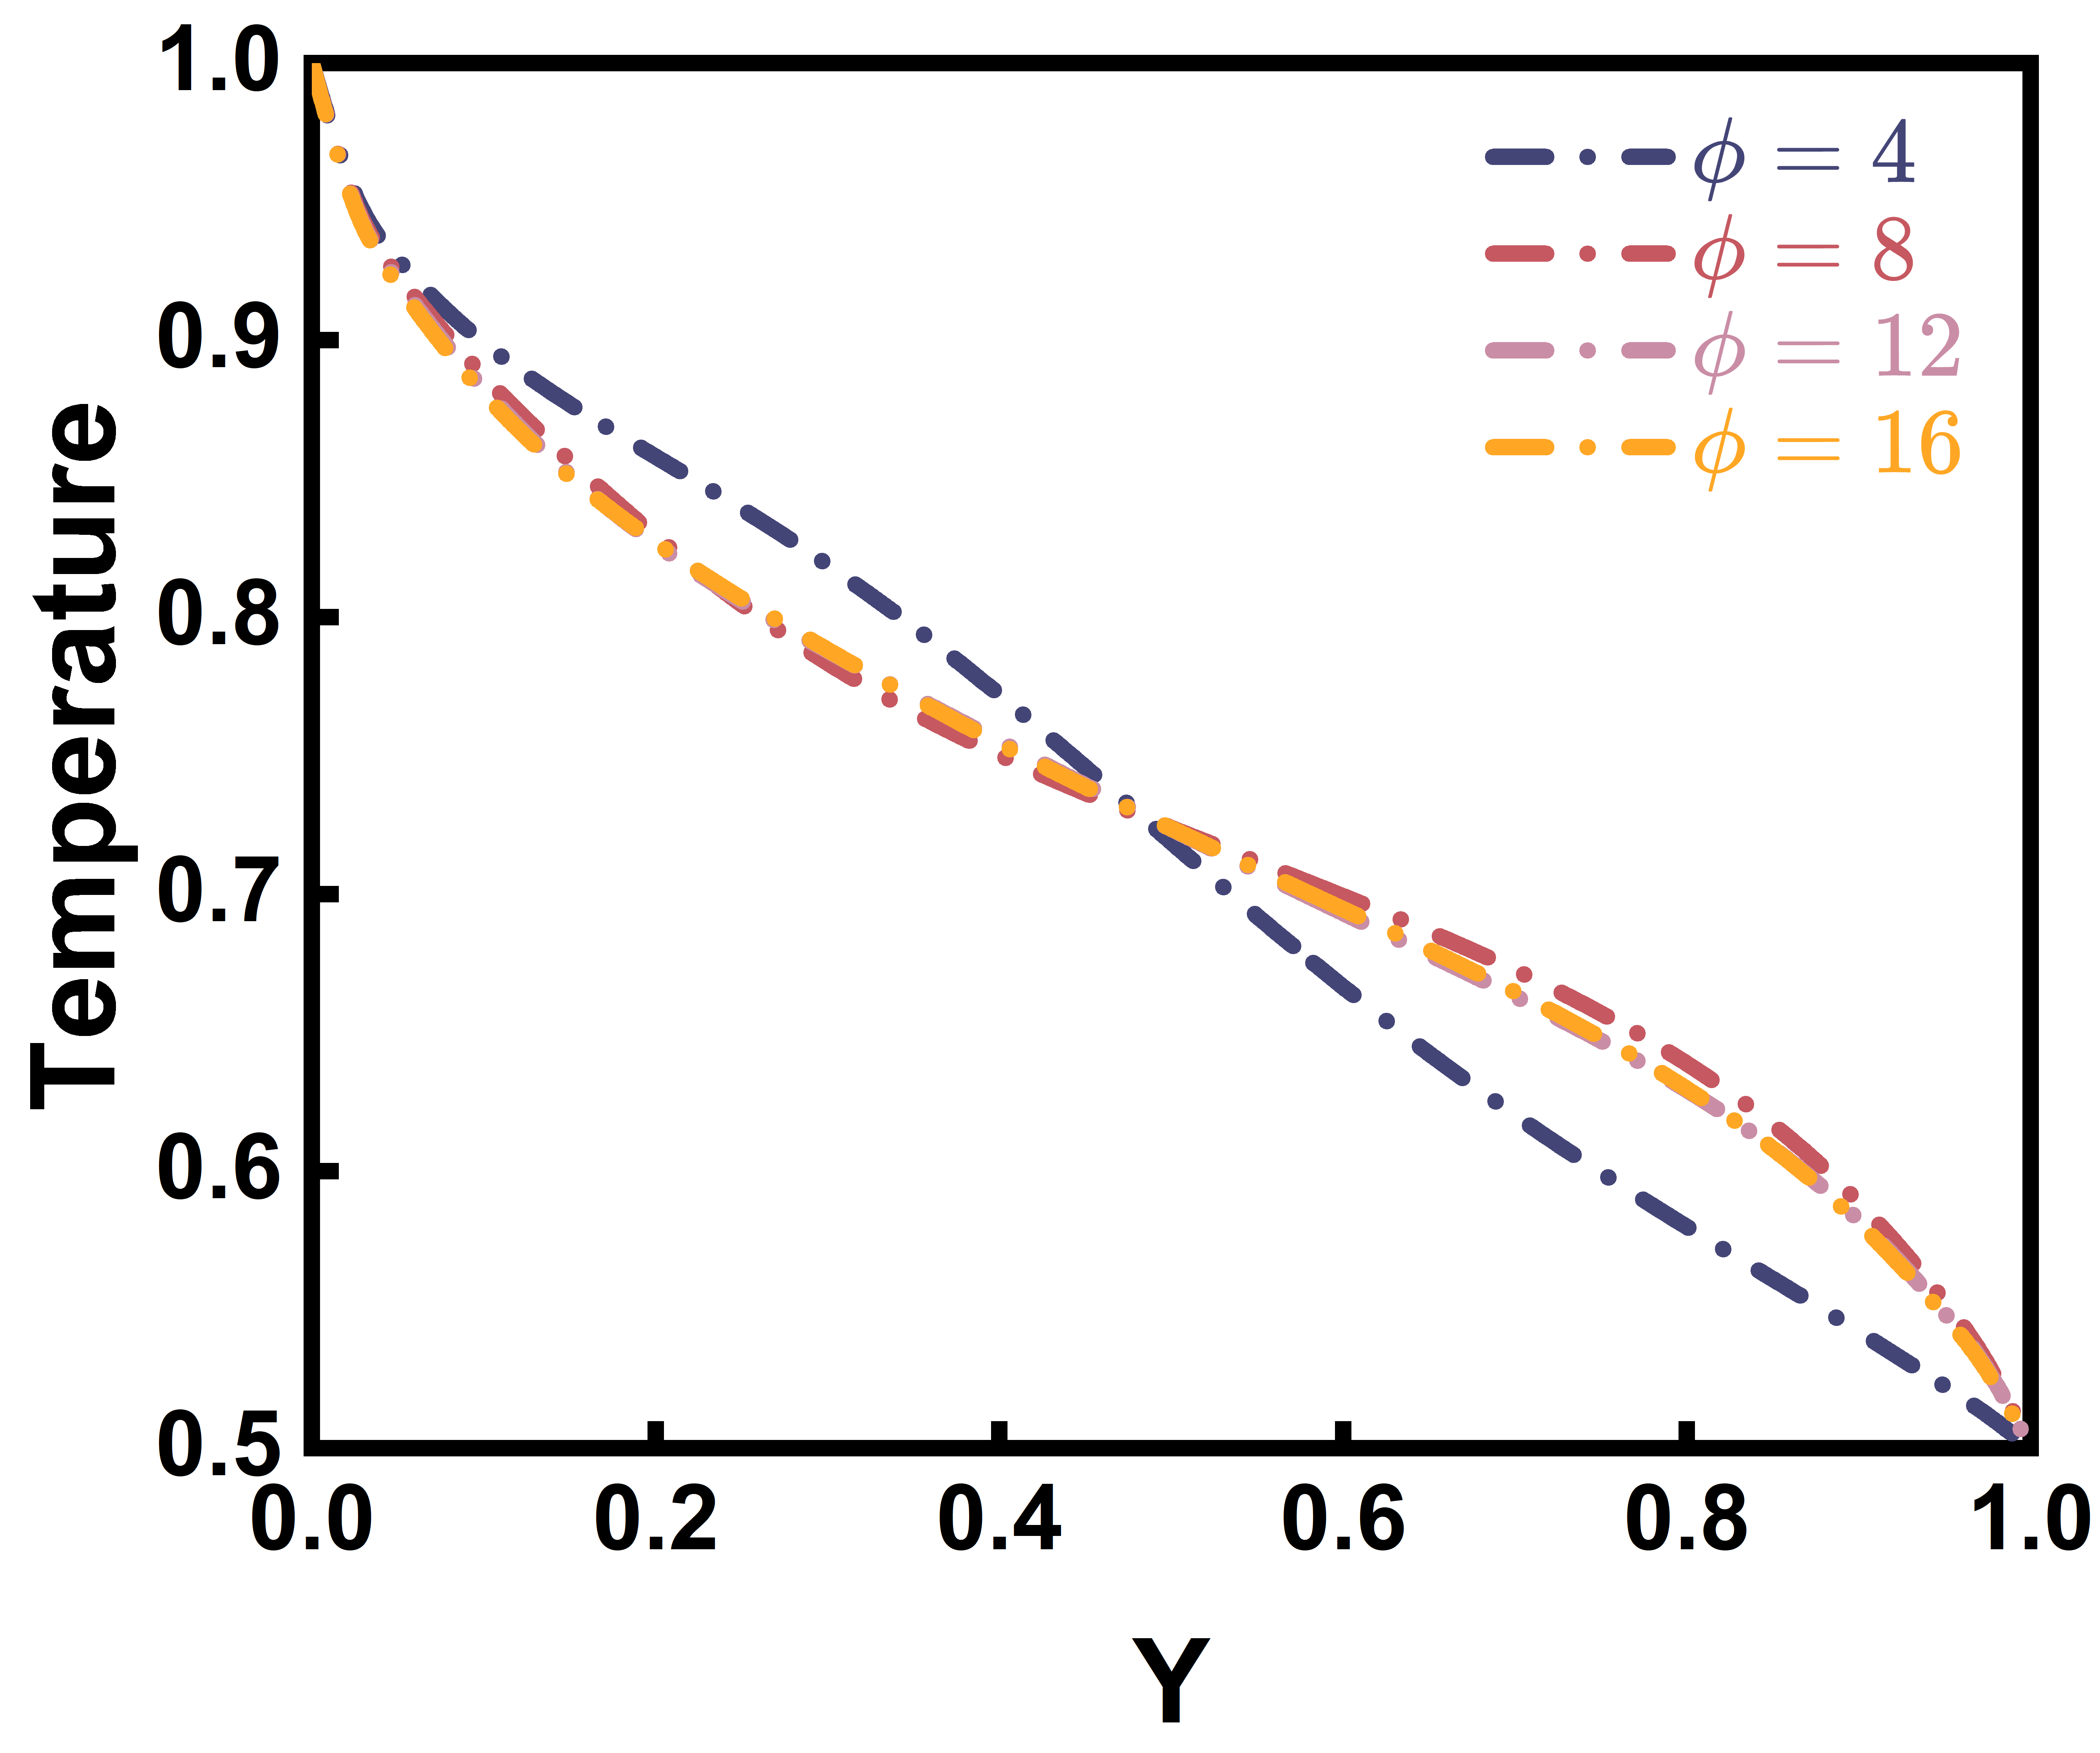
\includegraphics[width=\textwidth]{5A.png}
\caption{}
\end{subfigure}
\hfill
\begin{subfigure}[b]{\figwidth}
\centering
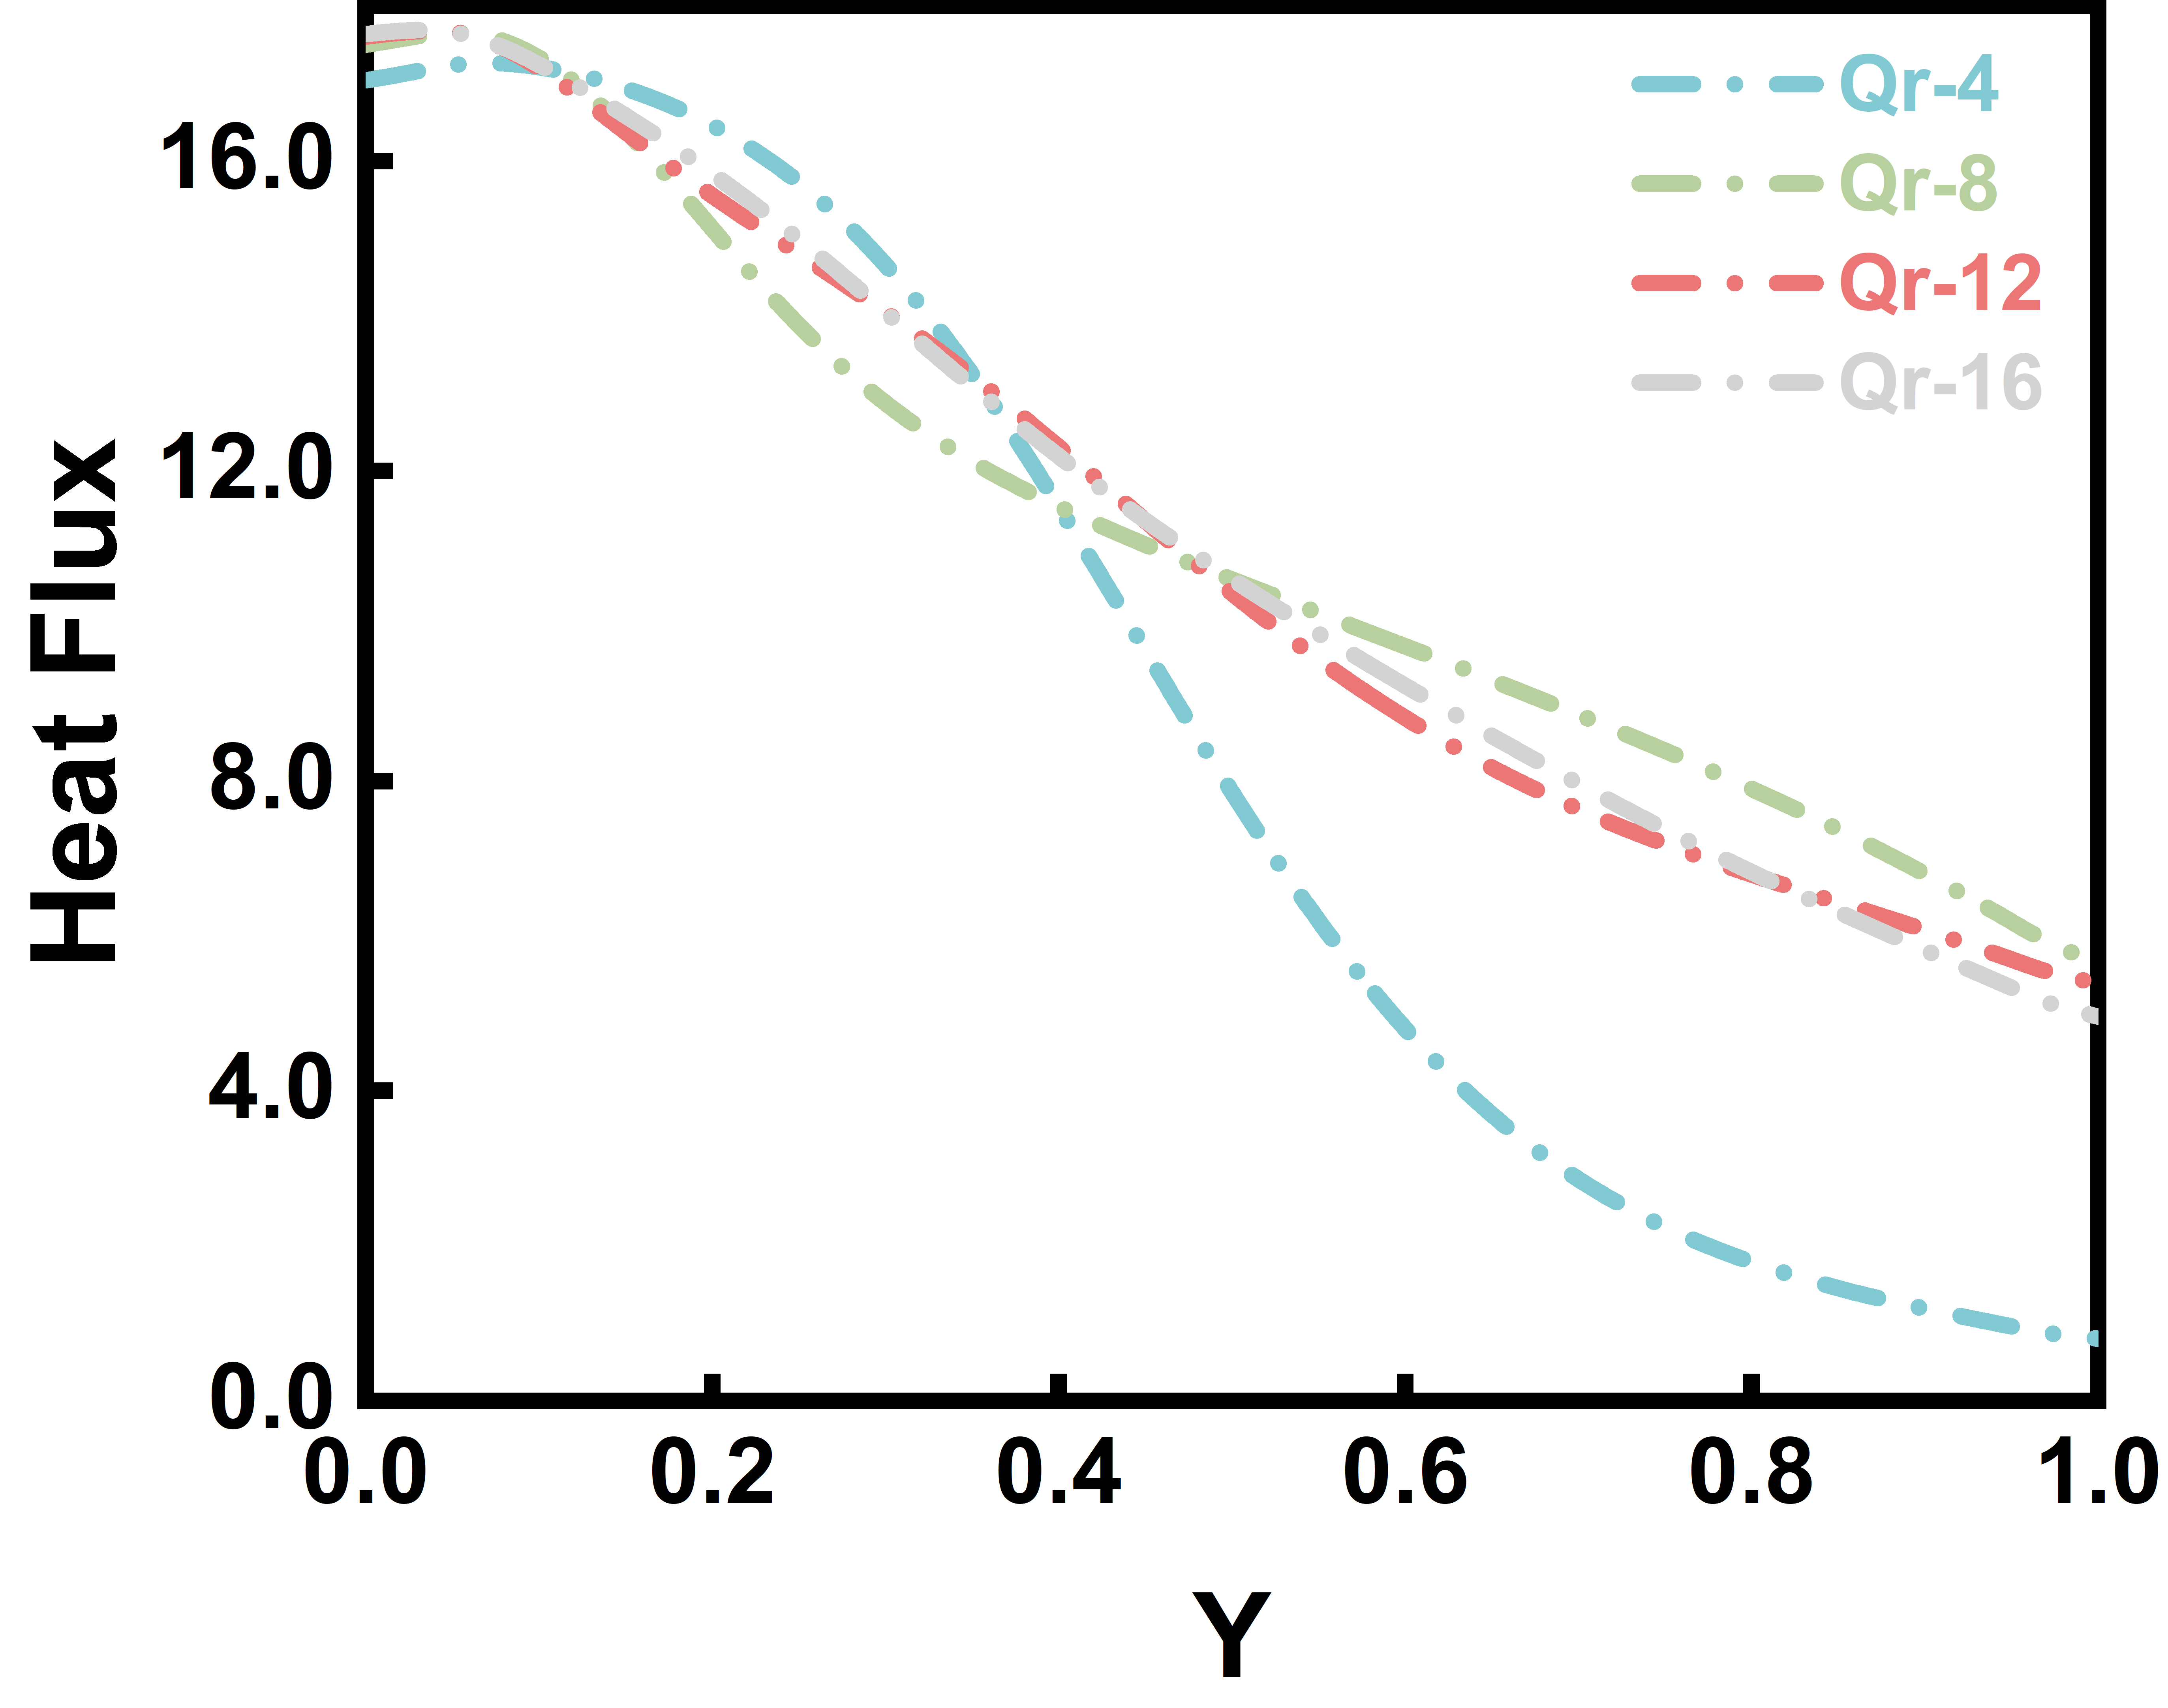
\includegraphics[width=\textwidth]{5B.png}
\caption{}
\end{subfigure}
\hfill
\begin{subfigure}[b]{\figwidth}
\centering
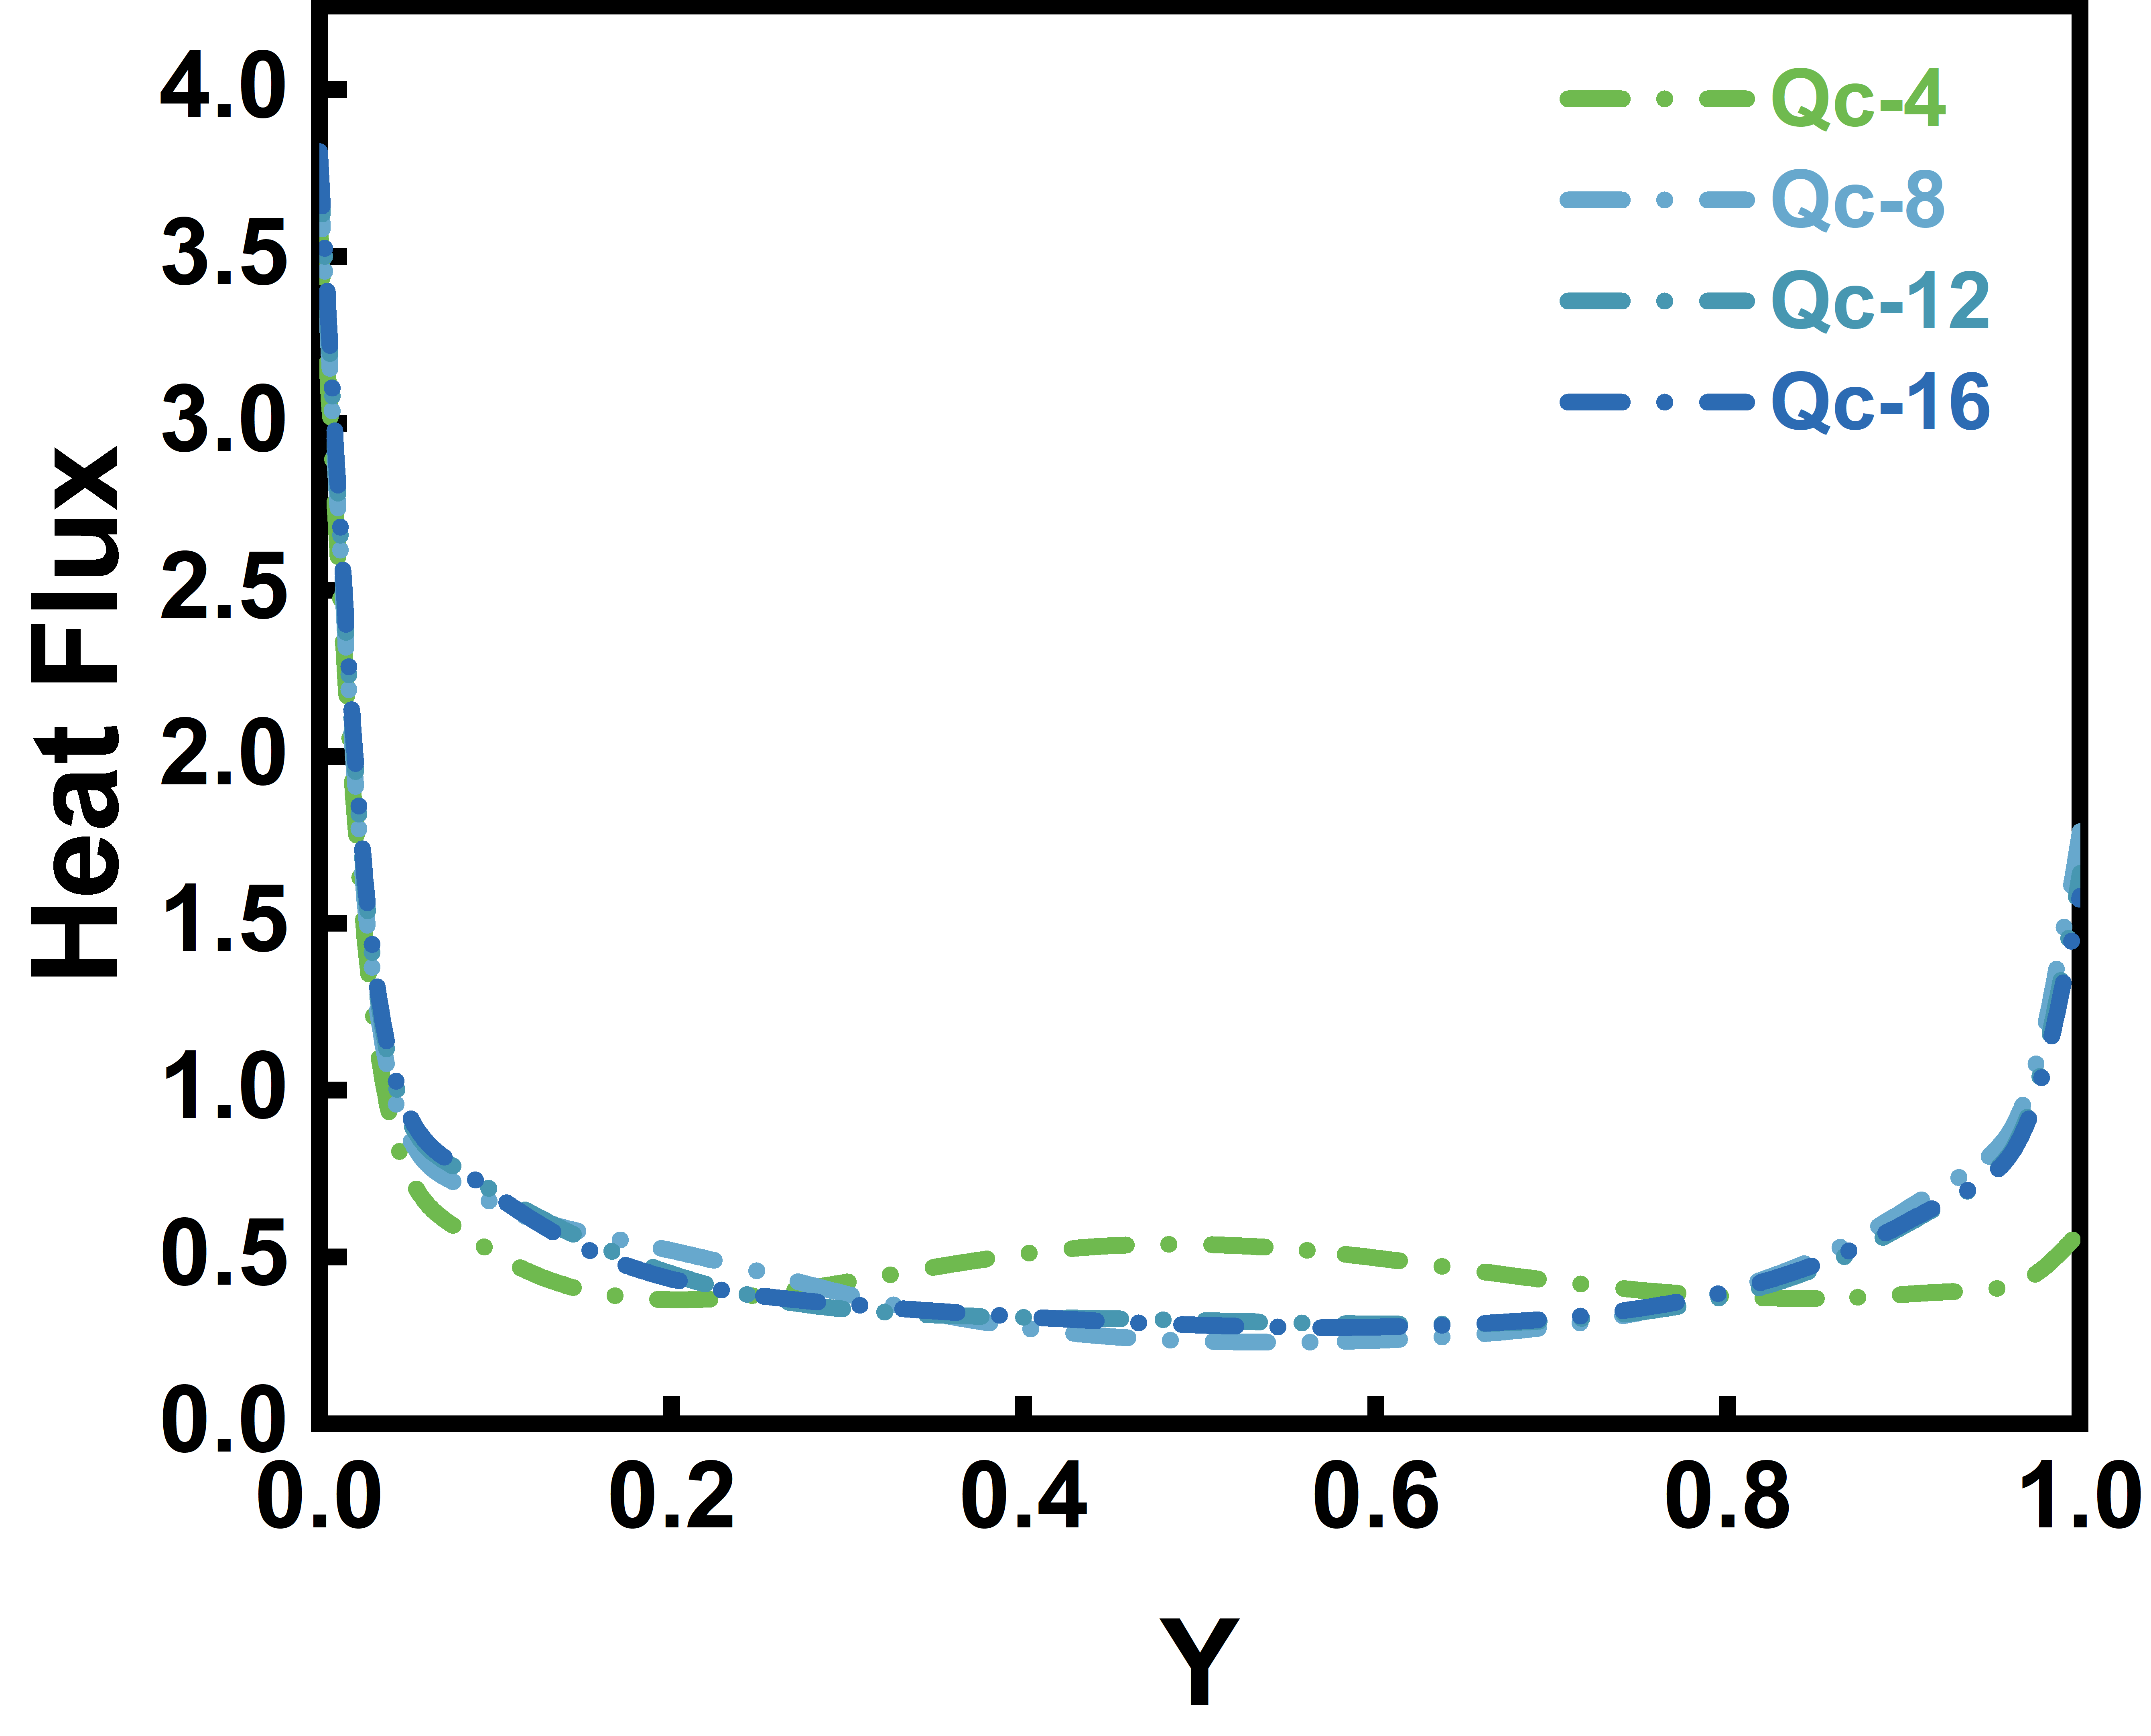
\includegraphics[width=\textwidth]{5C.png}
\caption{}
\end{subfigure}
\caption{Sensitivity of steady-state centreline profiles to azimuthal angular resolution in the two-dimensional square enclosure. The panels show (a) temperature, (b) radiative heat flux $q_r$,(c) conductive heat flux $q_c$. Calculations use $N=0.01$, $\omega=0$, $N_\theta=8$, and $N_\phi=4$, $8$, $12$, $16$.}
\label{fig5}
\end{figure}

Figure~\ref{fig5} compares centreline profiles for $N_\phi=4$, $8$, $12$, and $16$ azimuthal control volumes. The temperature profile changed markedly from $N_\phi=4$ to $N_\phi=8$. Differences among $N_\phi=8$, $12$, and $16$ were smaller. The heat-flux profiles were more sensitive, with visible differences remaining between $N_\phi=8$ and the finer discretisations. All subsequent two-dimensional calculations therefore used $N_\phi=16$.

\begin{figure}[H]
\centering
\begin{subfigure}[b]{\figwidth}
\centering
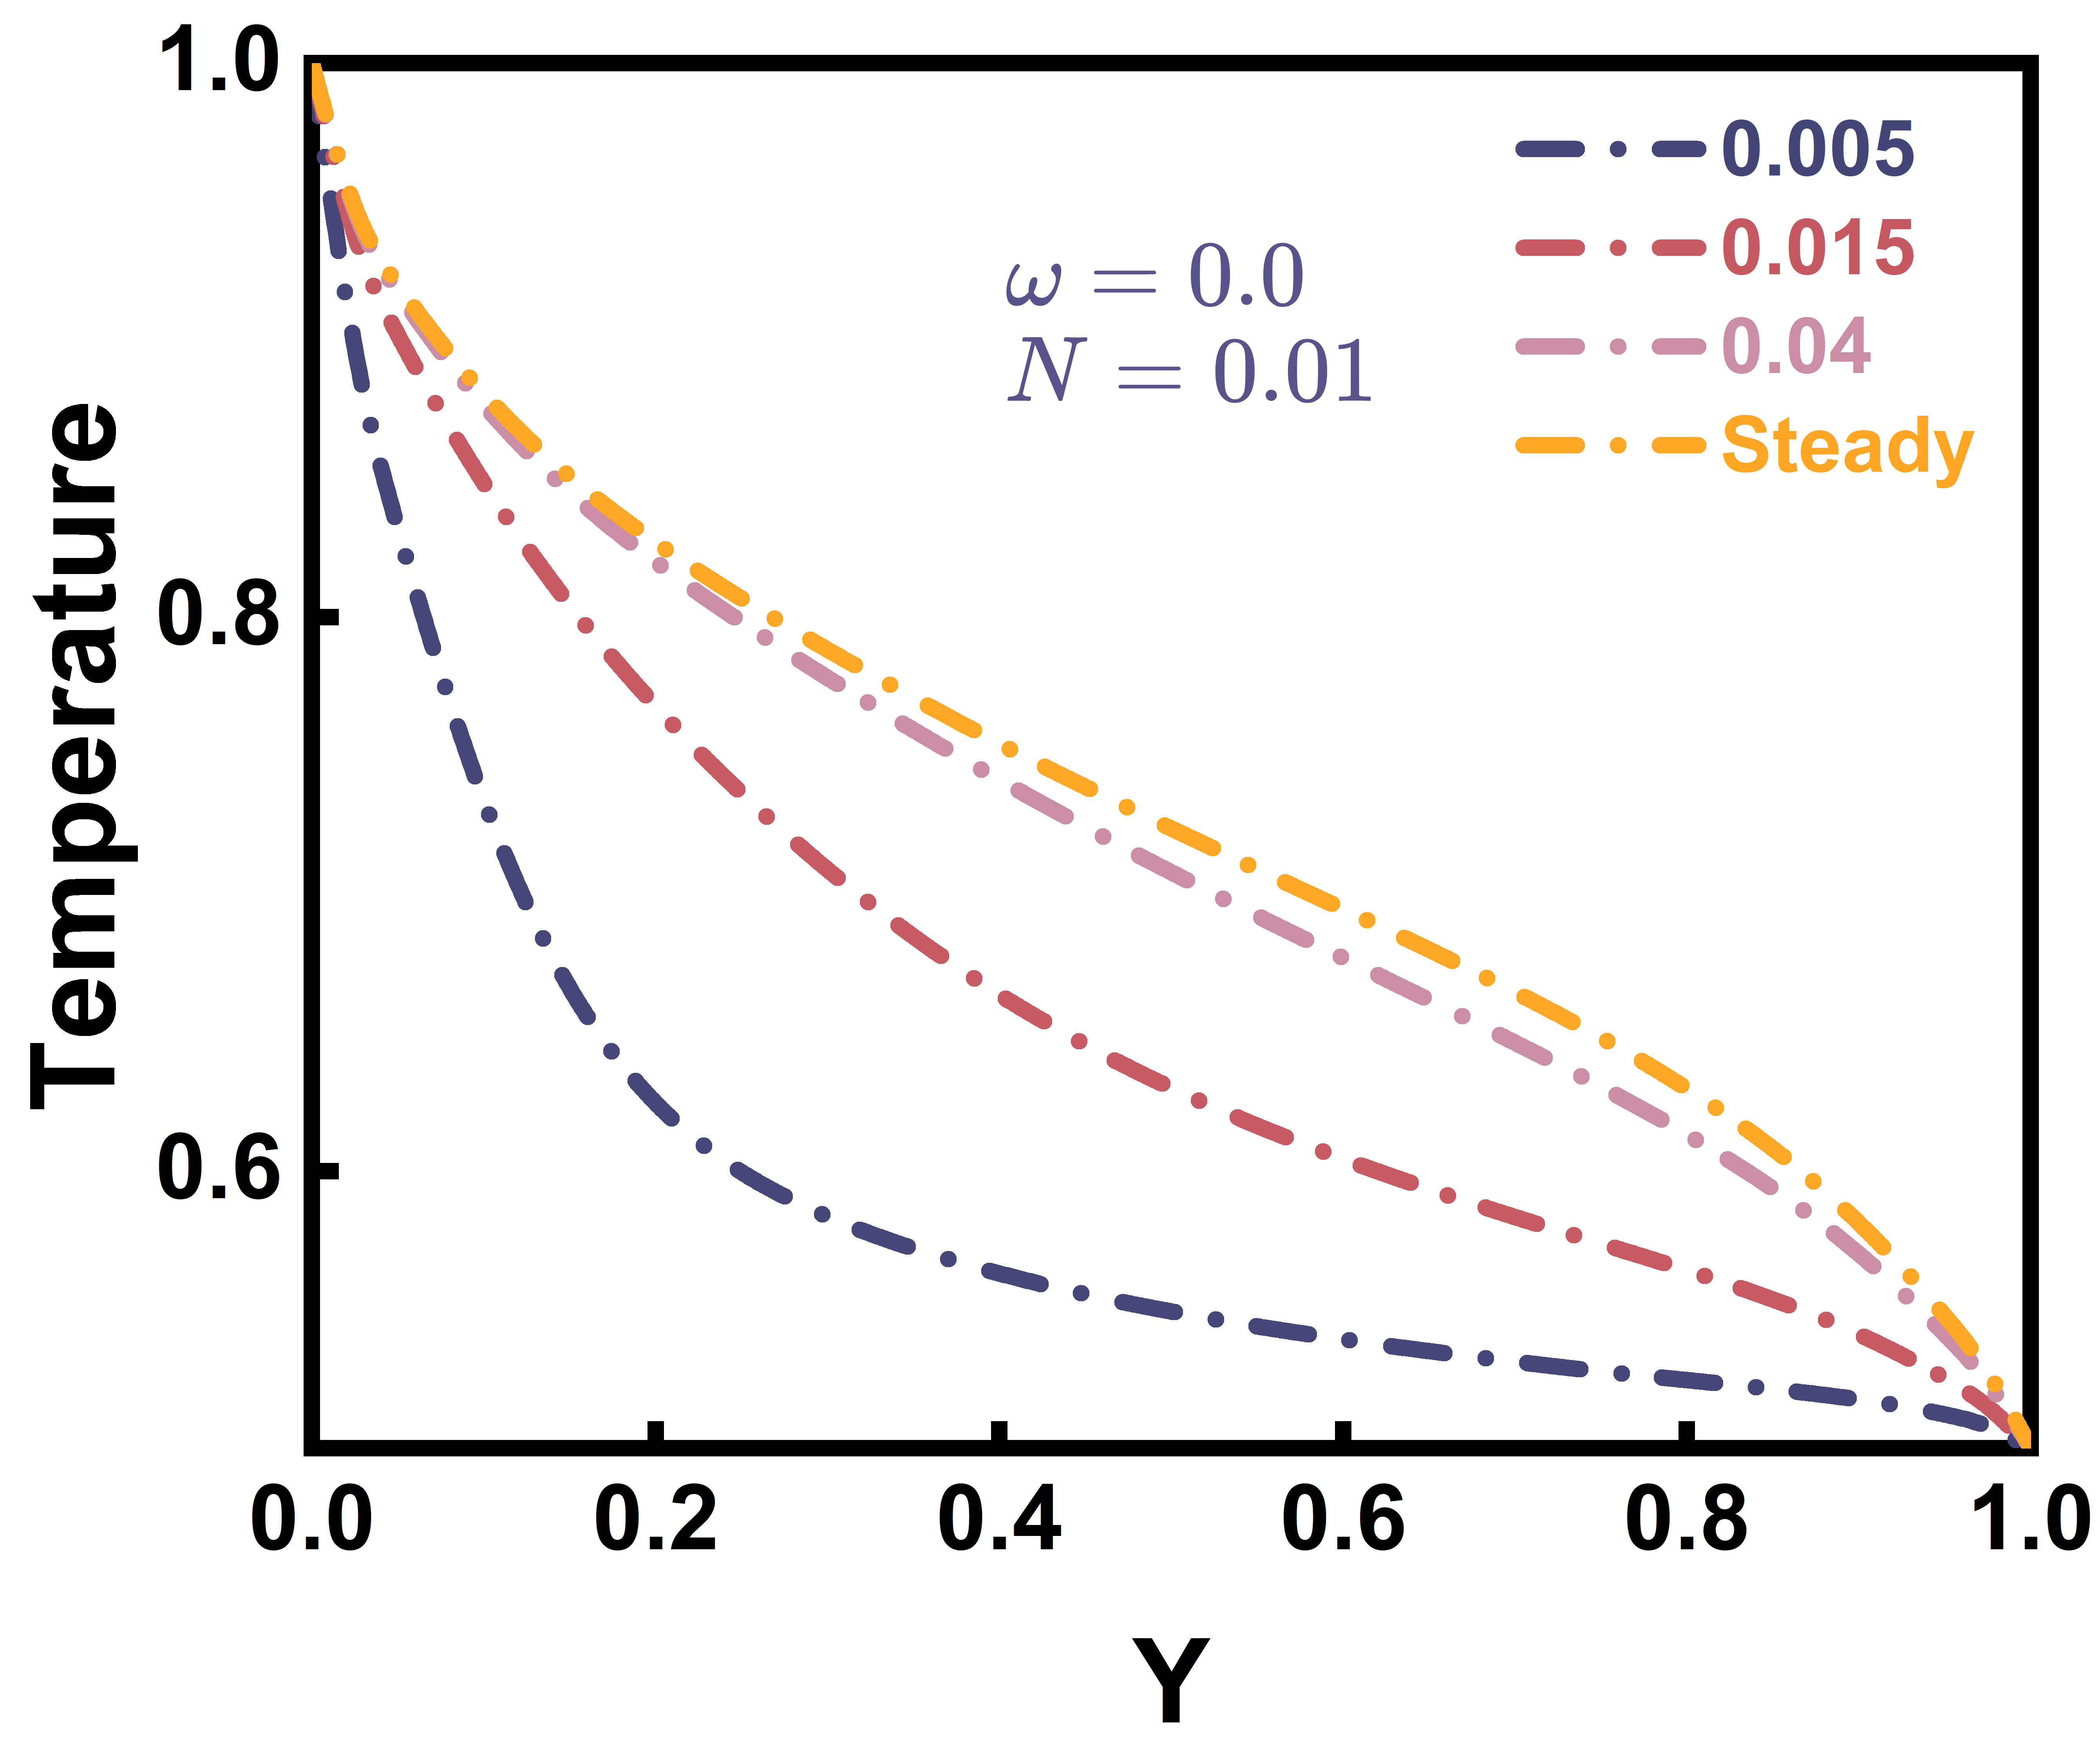
\includegraphics[width=\textwidth]{6A.png}
\caption{}
\end{subfigure}
\hfill
\begin{subfigure}[b]{\figwidth}
\centering
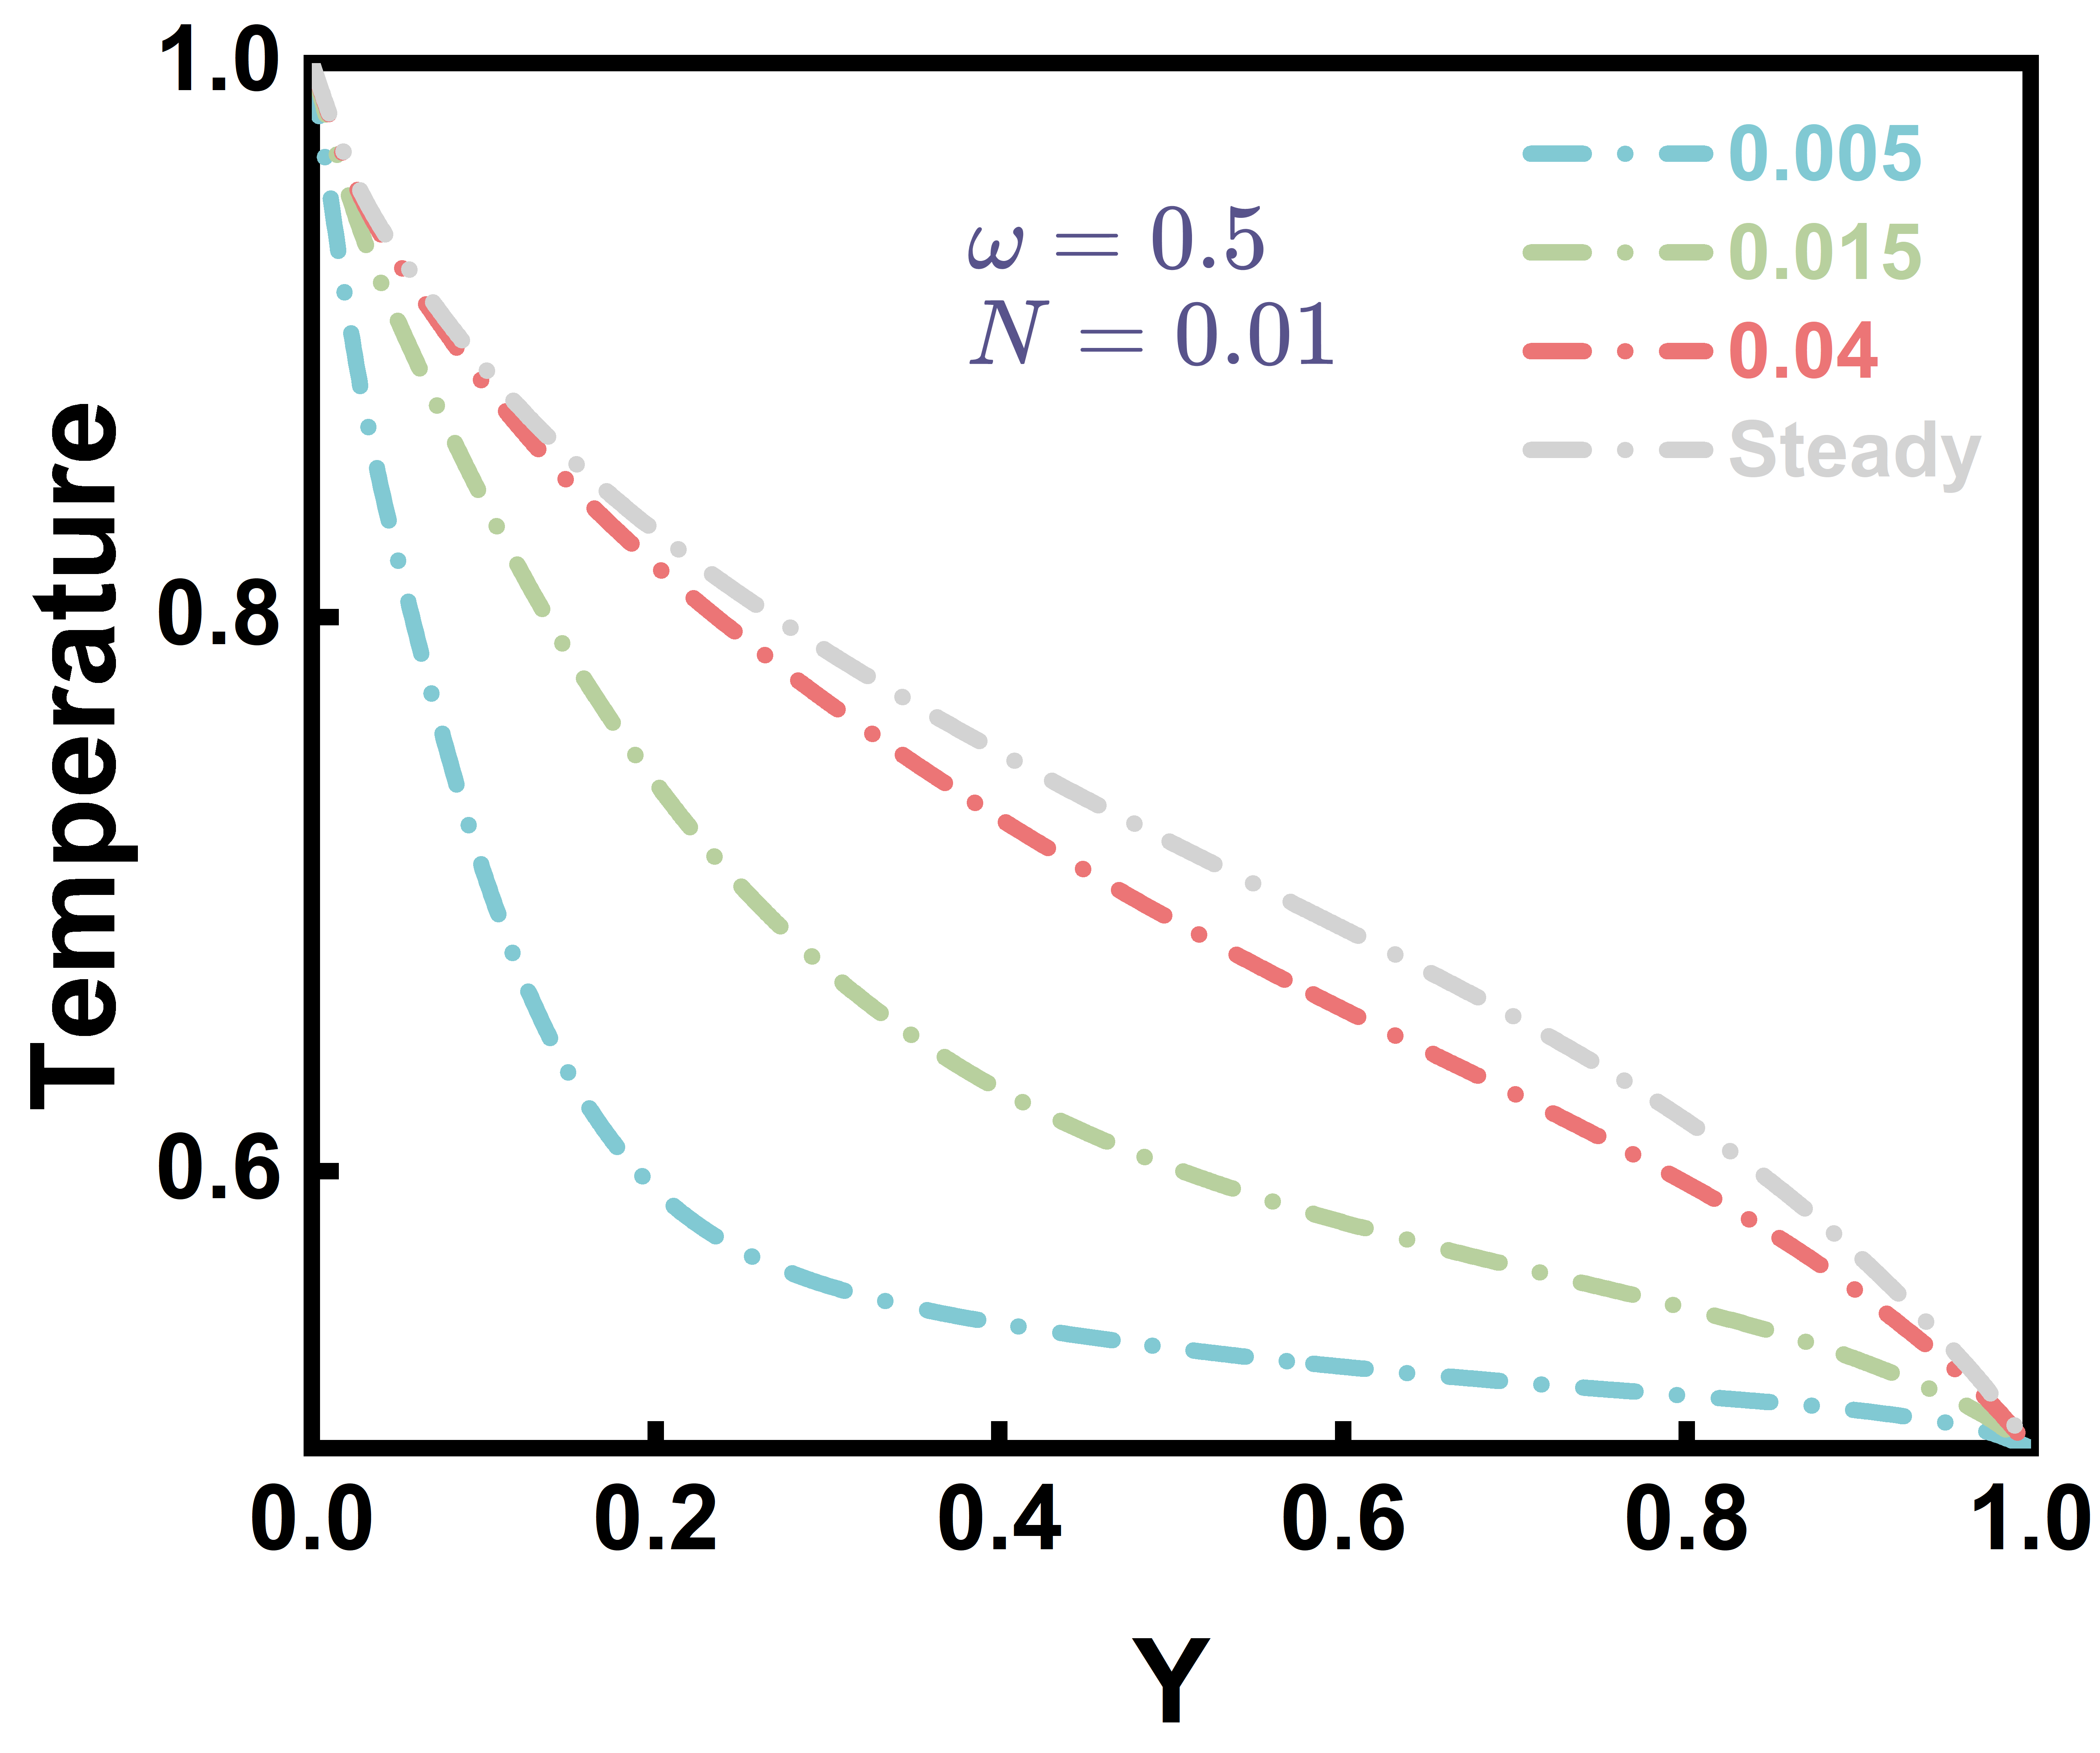
\includegraphics[width=\textwidth]{6B.png}
\caption{}
\end{subfigure}
\hfill
\begin{subfigure}[b]{\figwidth}
\centering
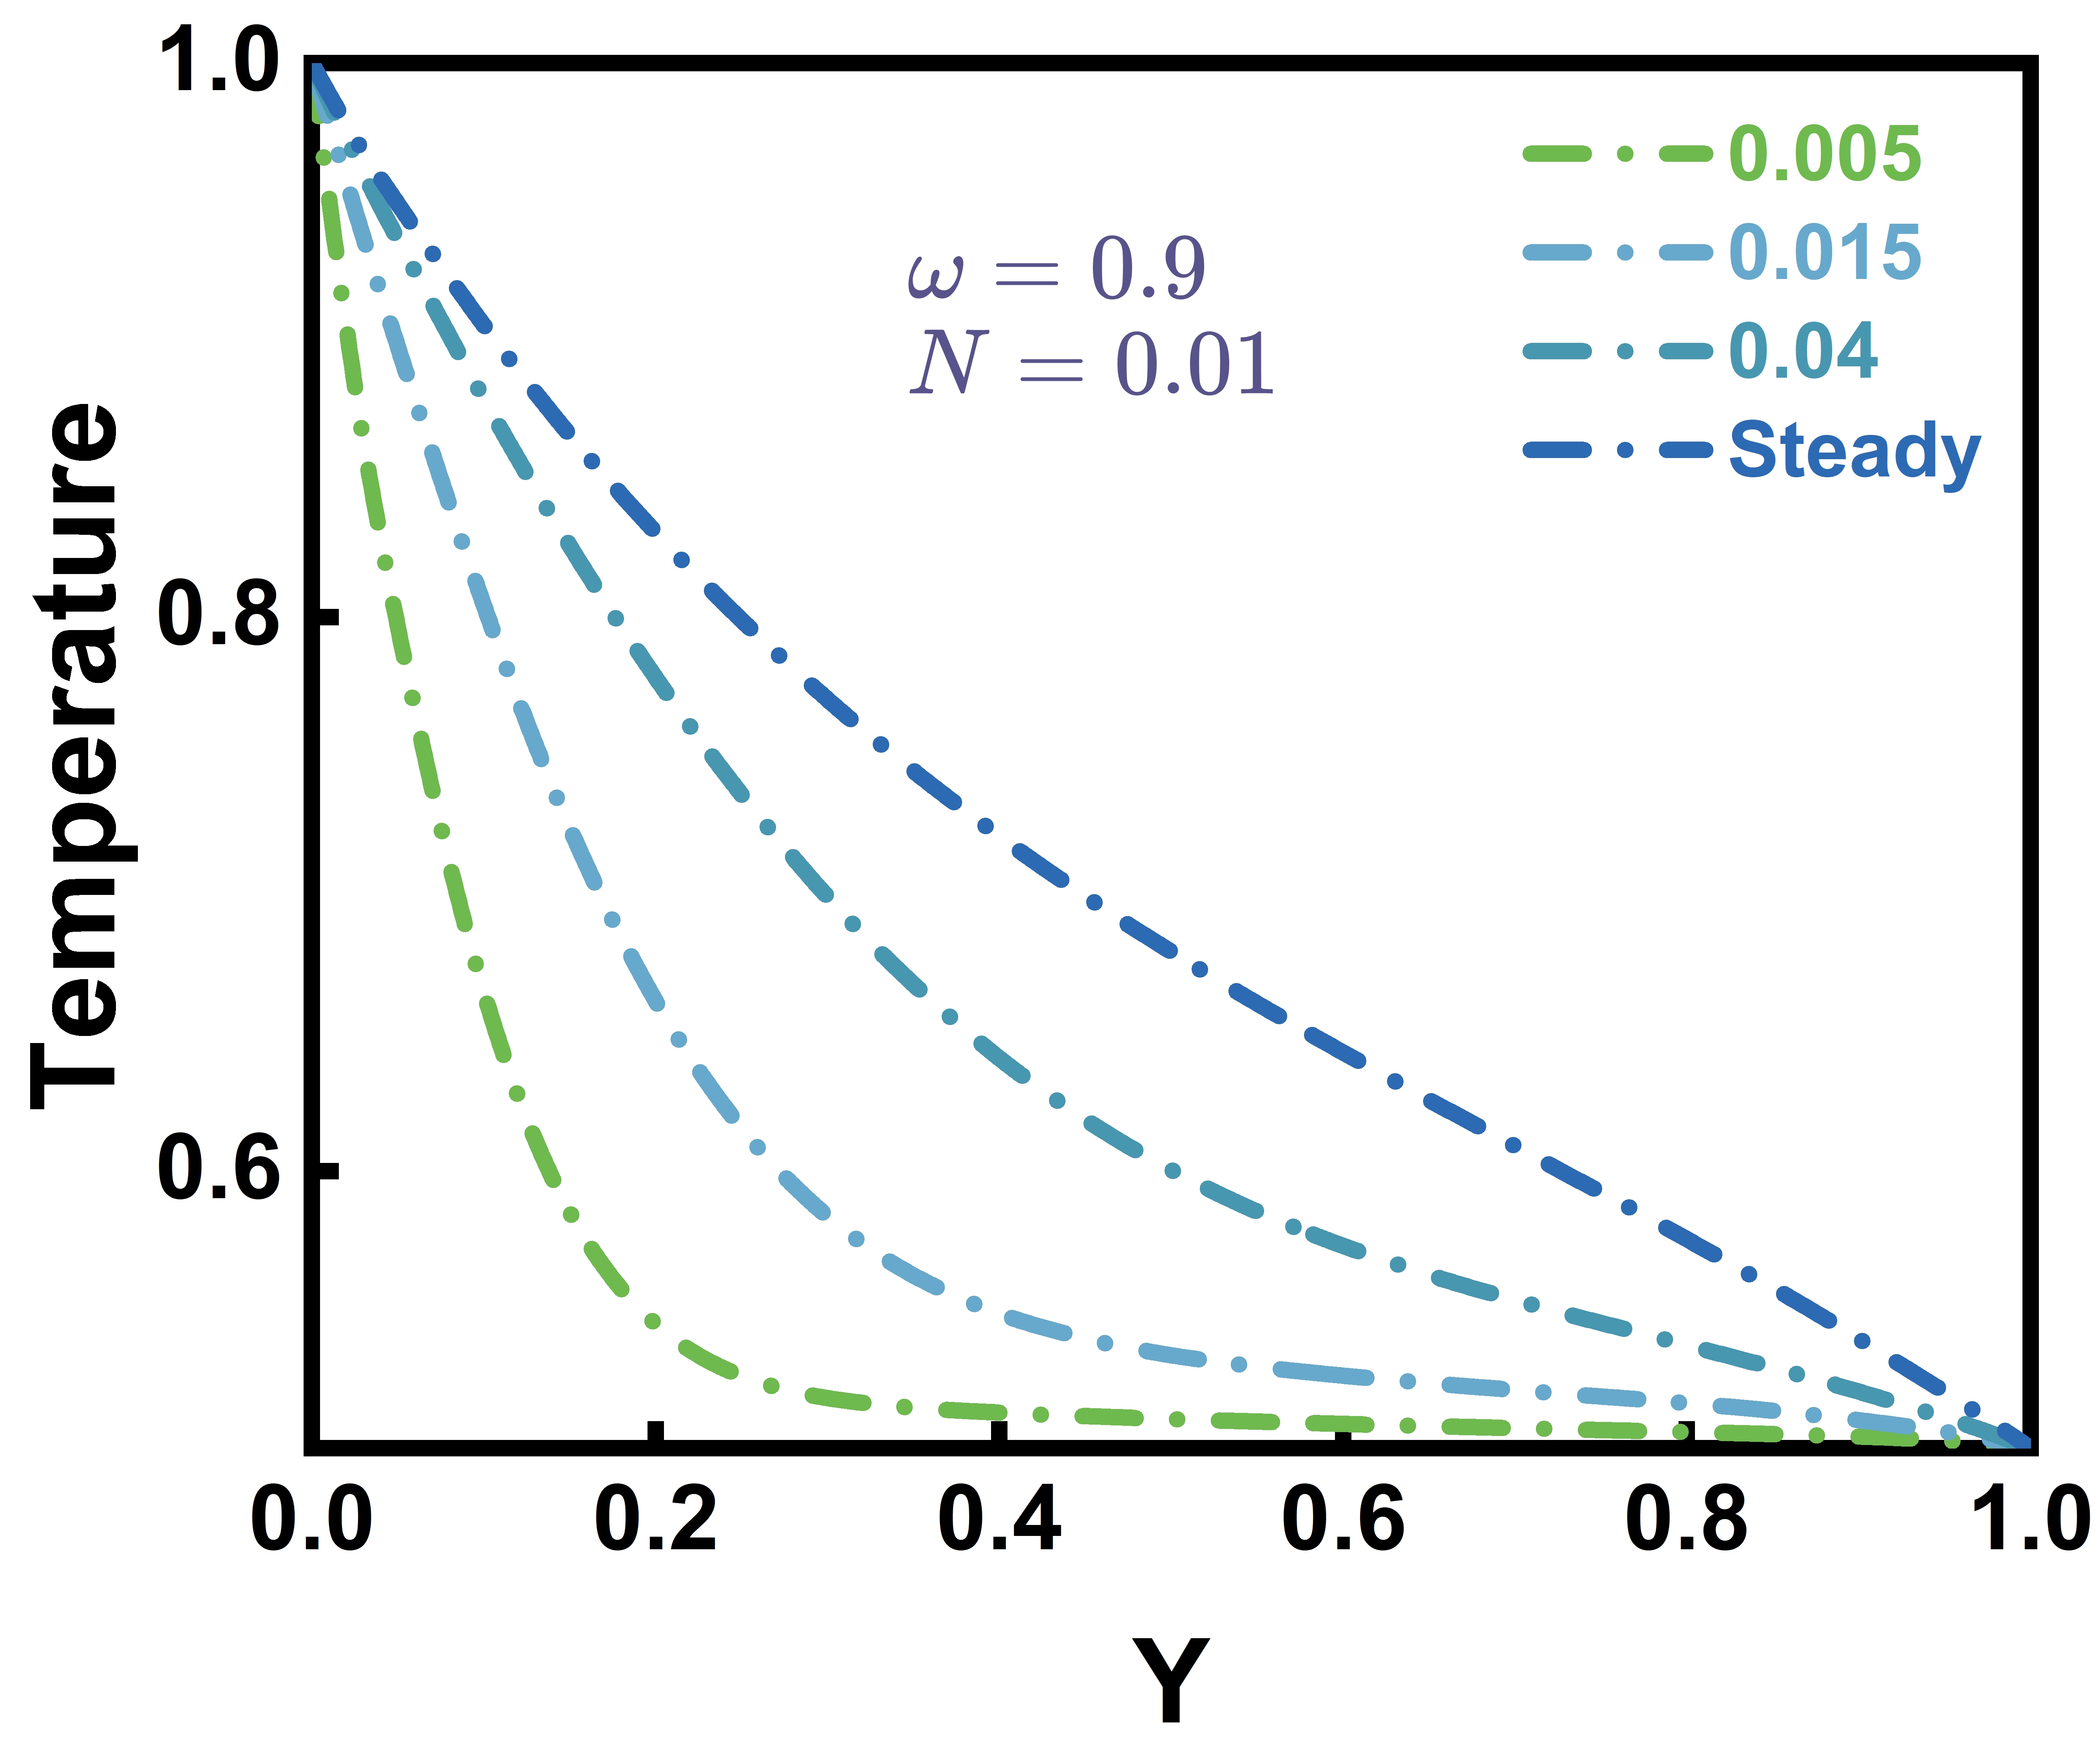
\includegraphics[width=\textwidth]{6C.png}
\caption{}
\end{subfigure}
\caption{Transient centreline temperature profiles in the two-dimensional square enclosure at $N=0.01$ ,$T_0=0.5$. The scattering albedo is (a) $\omega=0$, (b) $\omega=0.5$,(c) $\omega=0.9$.}
\label{fig6}
\end{figure}

Figure~\ref{fig6} shows transient centreline temperatures for different scattering albedos. Increasing $\omega$ lowered the temperature and increased the time required to approach steady state. The two-dimensional temperatures were lower than their one-dimensional counterparts under corresponding conditions. At lower $\omega$, the steady-state temperature gradient near the north wall was larger.

\begin{figure}[H]
\centering
\begin{subfigure}[b]{\figwidth}
\centering
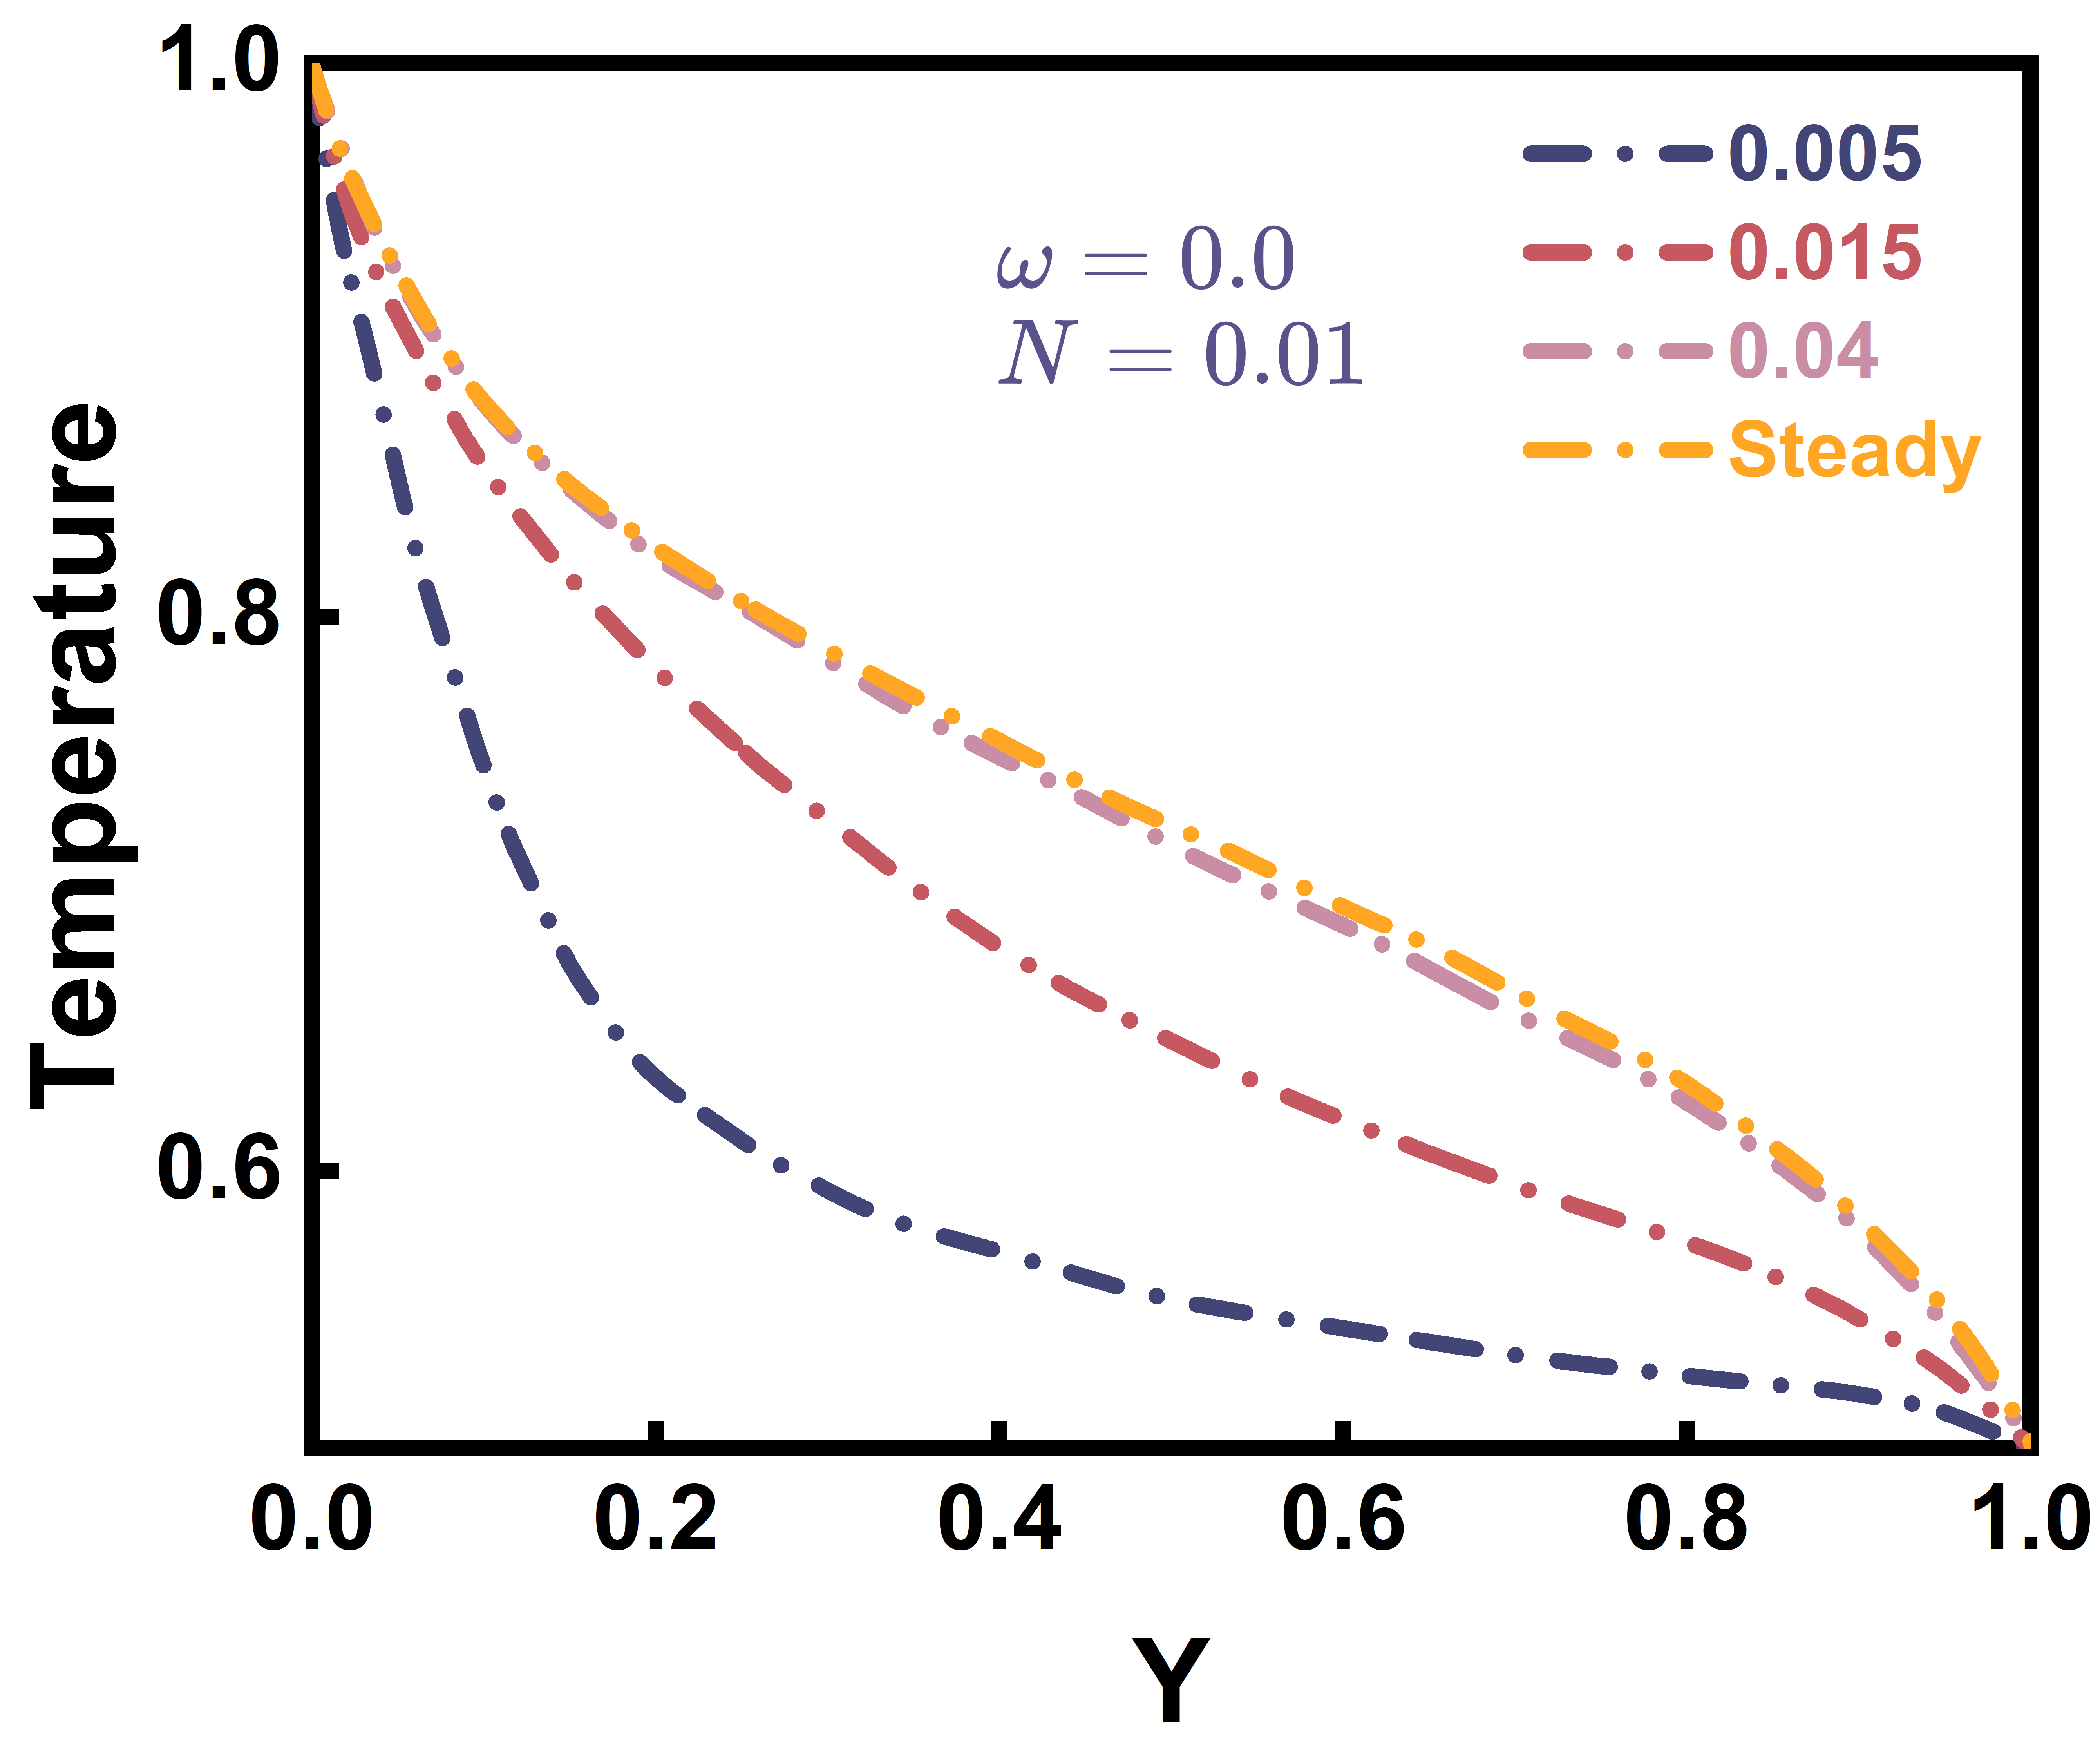
\includegraphics[width=\textwidth]{7A.png}
\caption{}
\end{subfigure}
\hfill
\begin{subfigure}[b]{\figwidth}
\centering
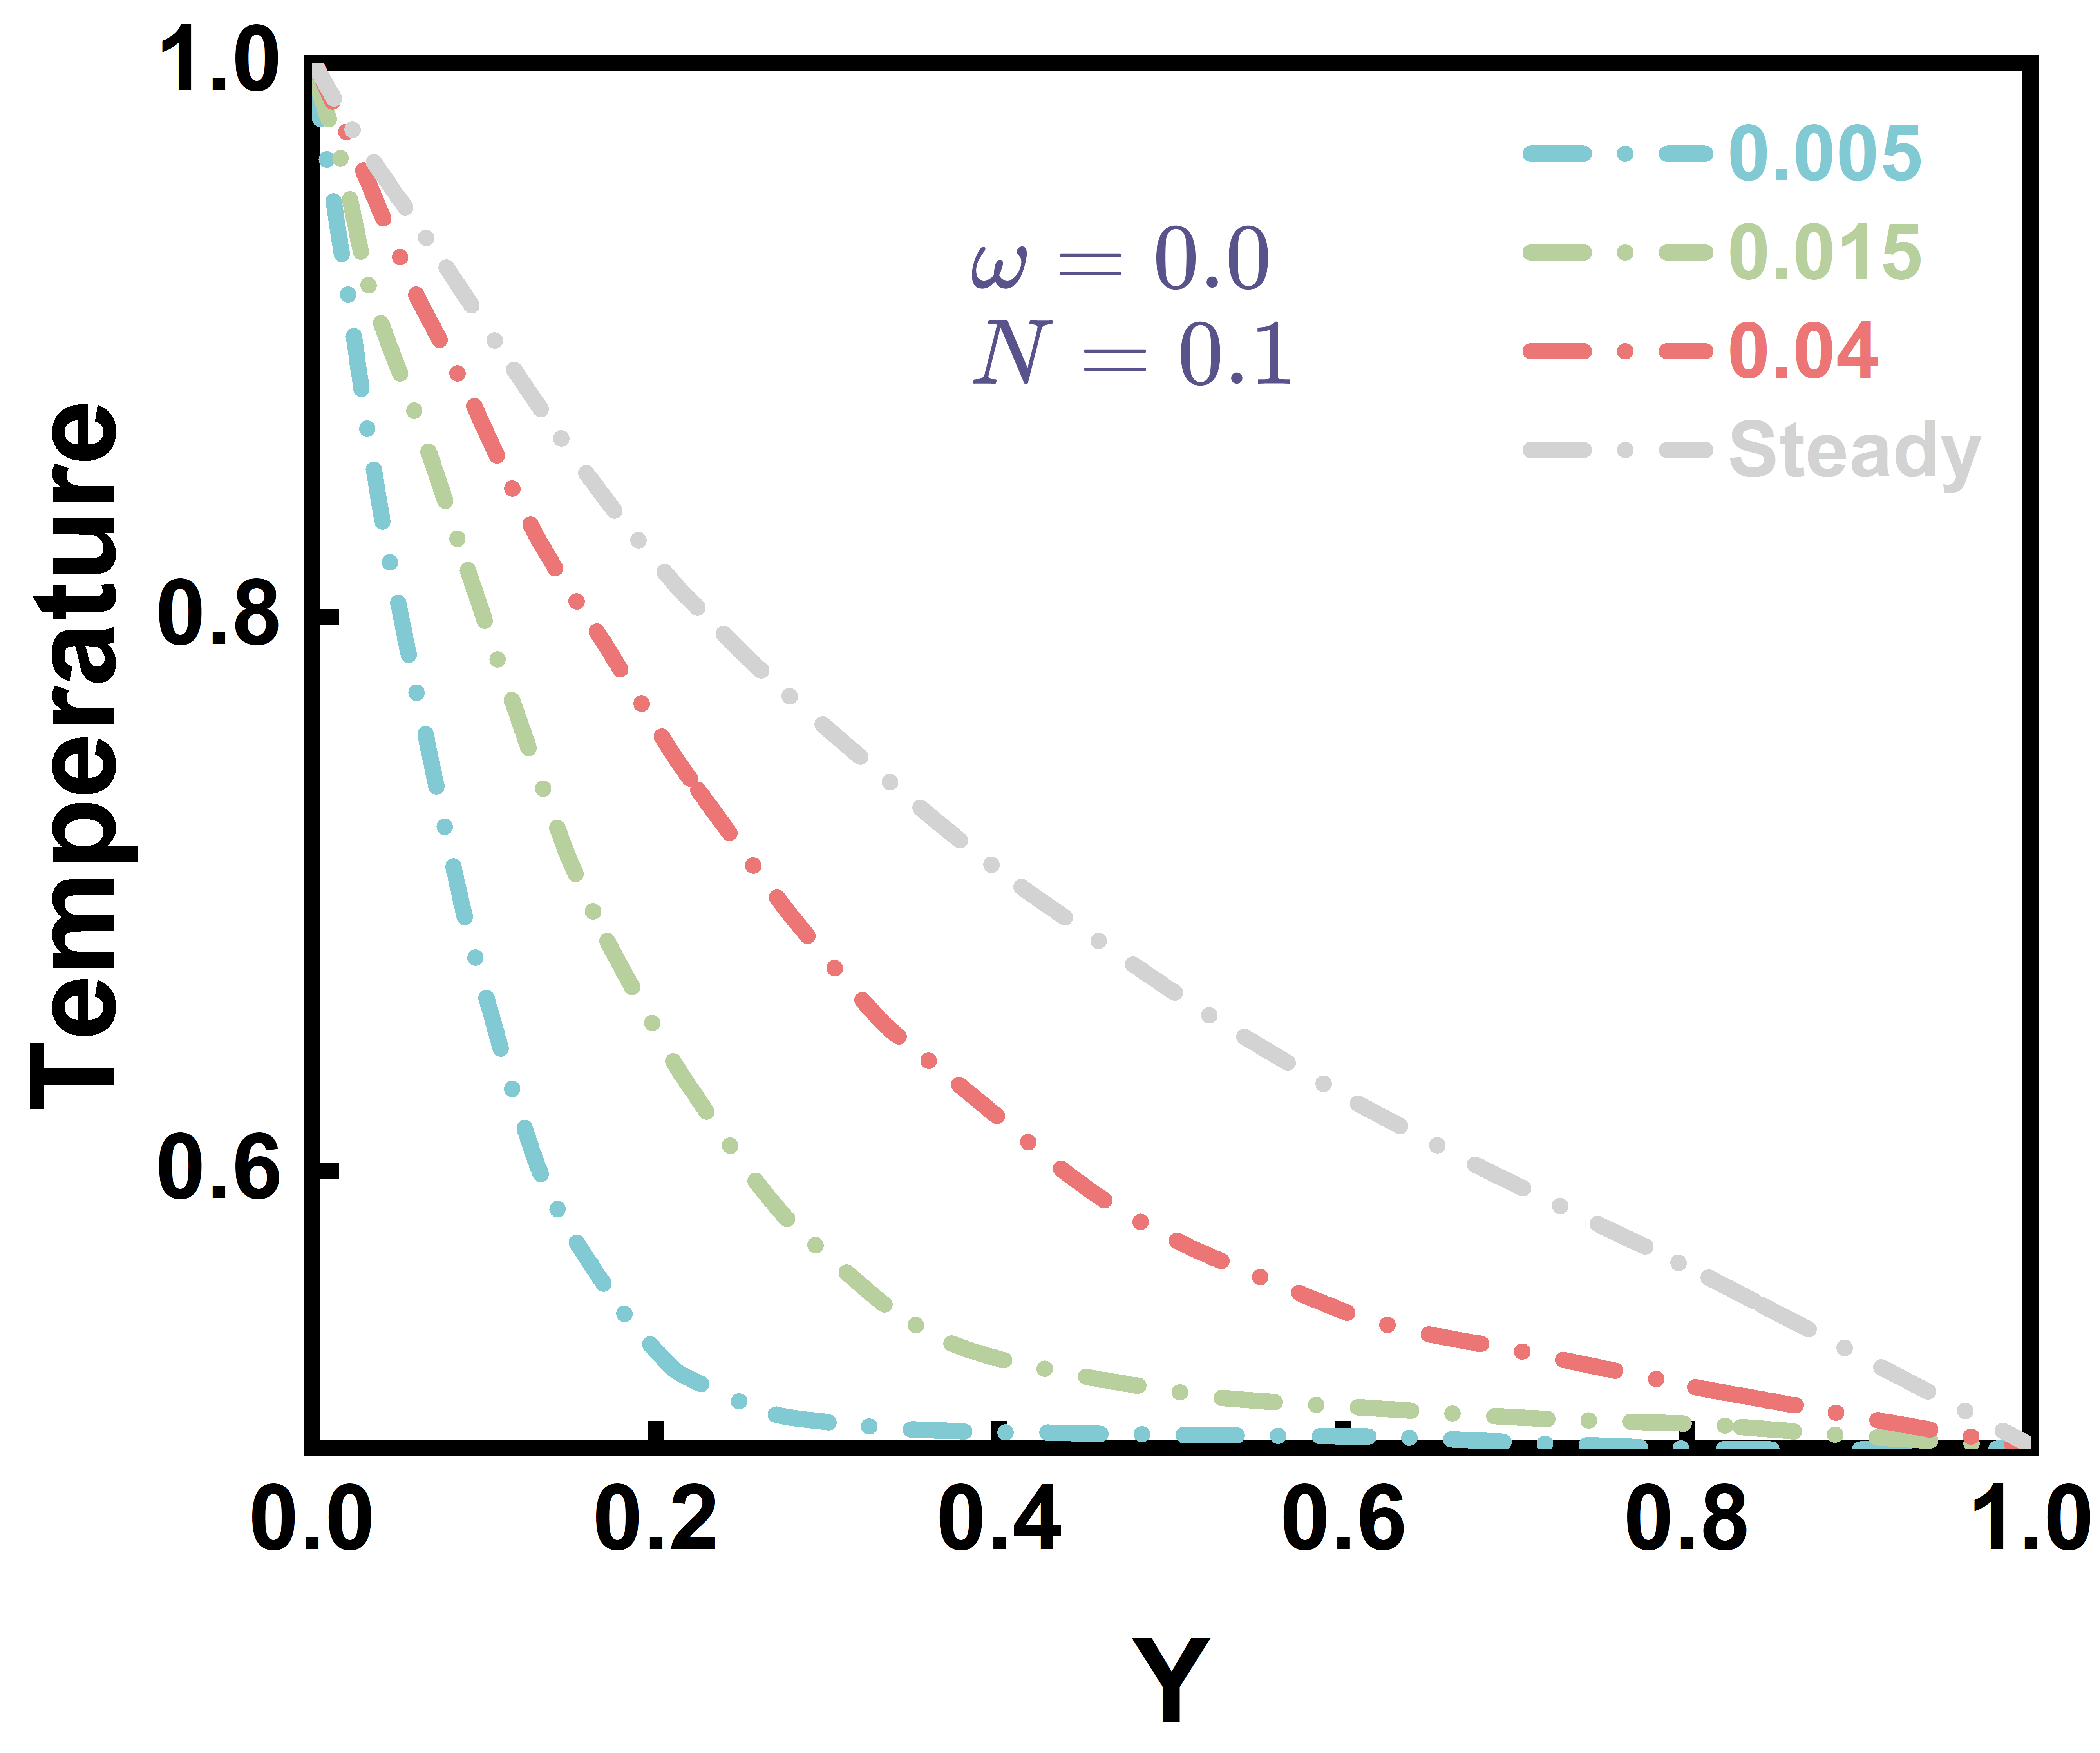
\includegraphics[width=\textwidth]{7B.png}
\caption{}
\end{subfigure}
\hfill
\begin{subfigure}[b]{\figwidth}
\centering
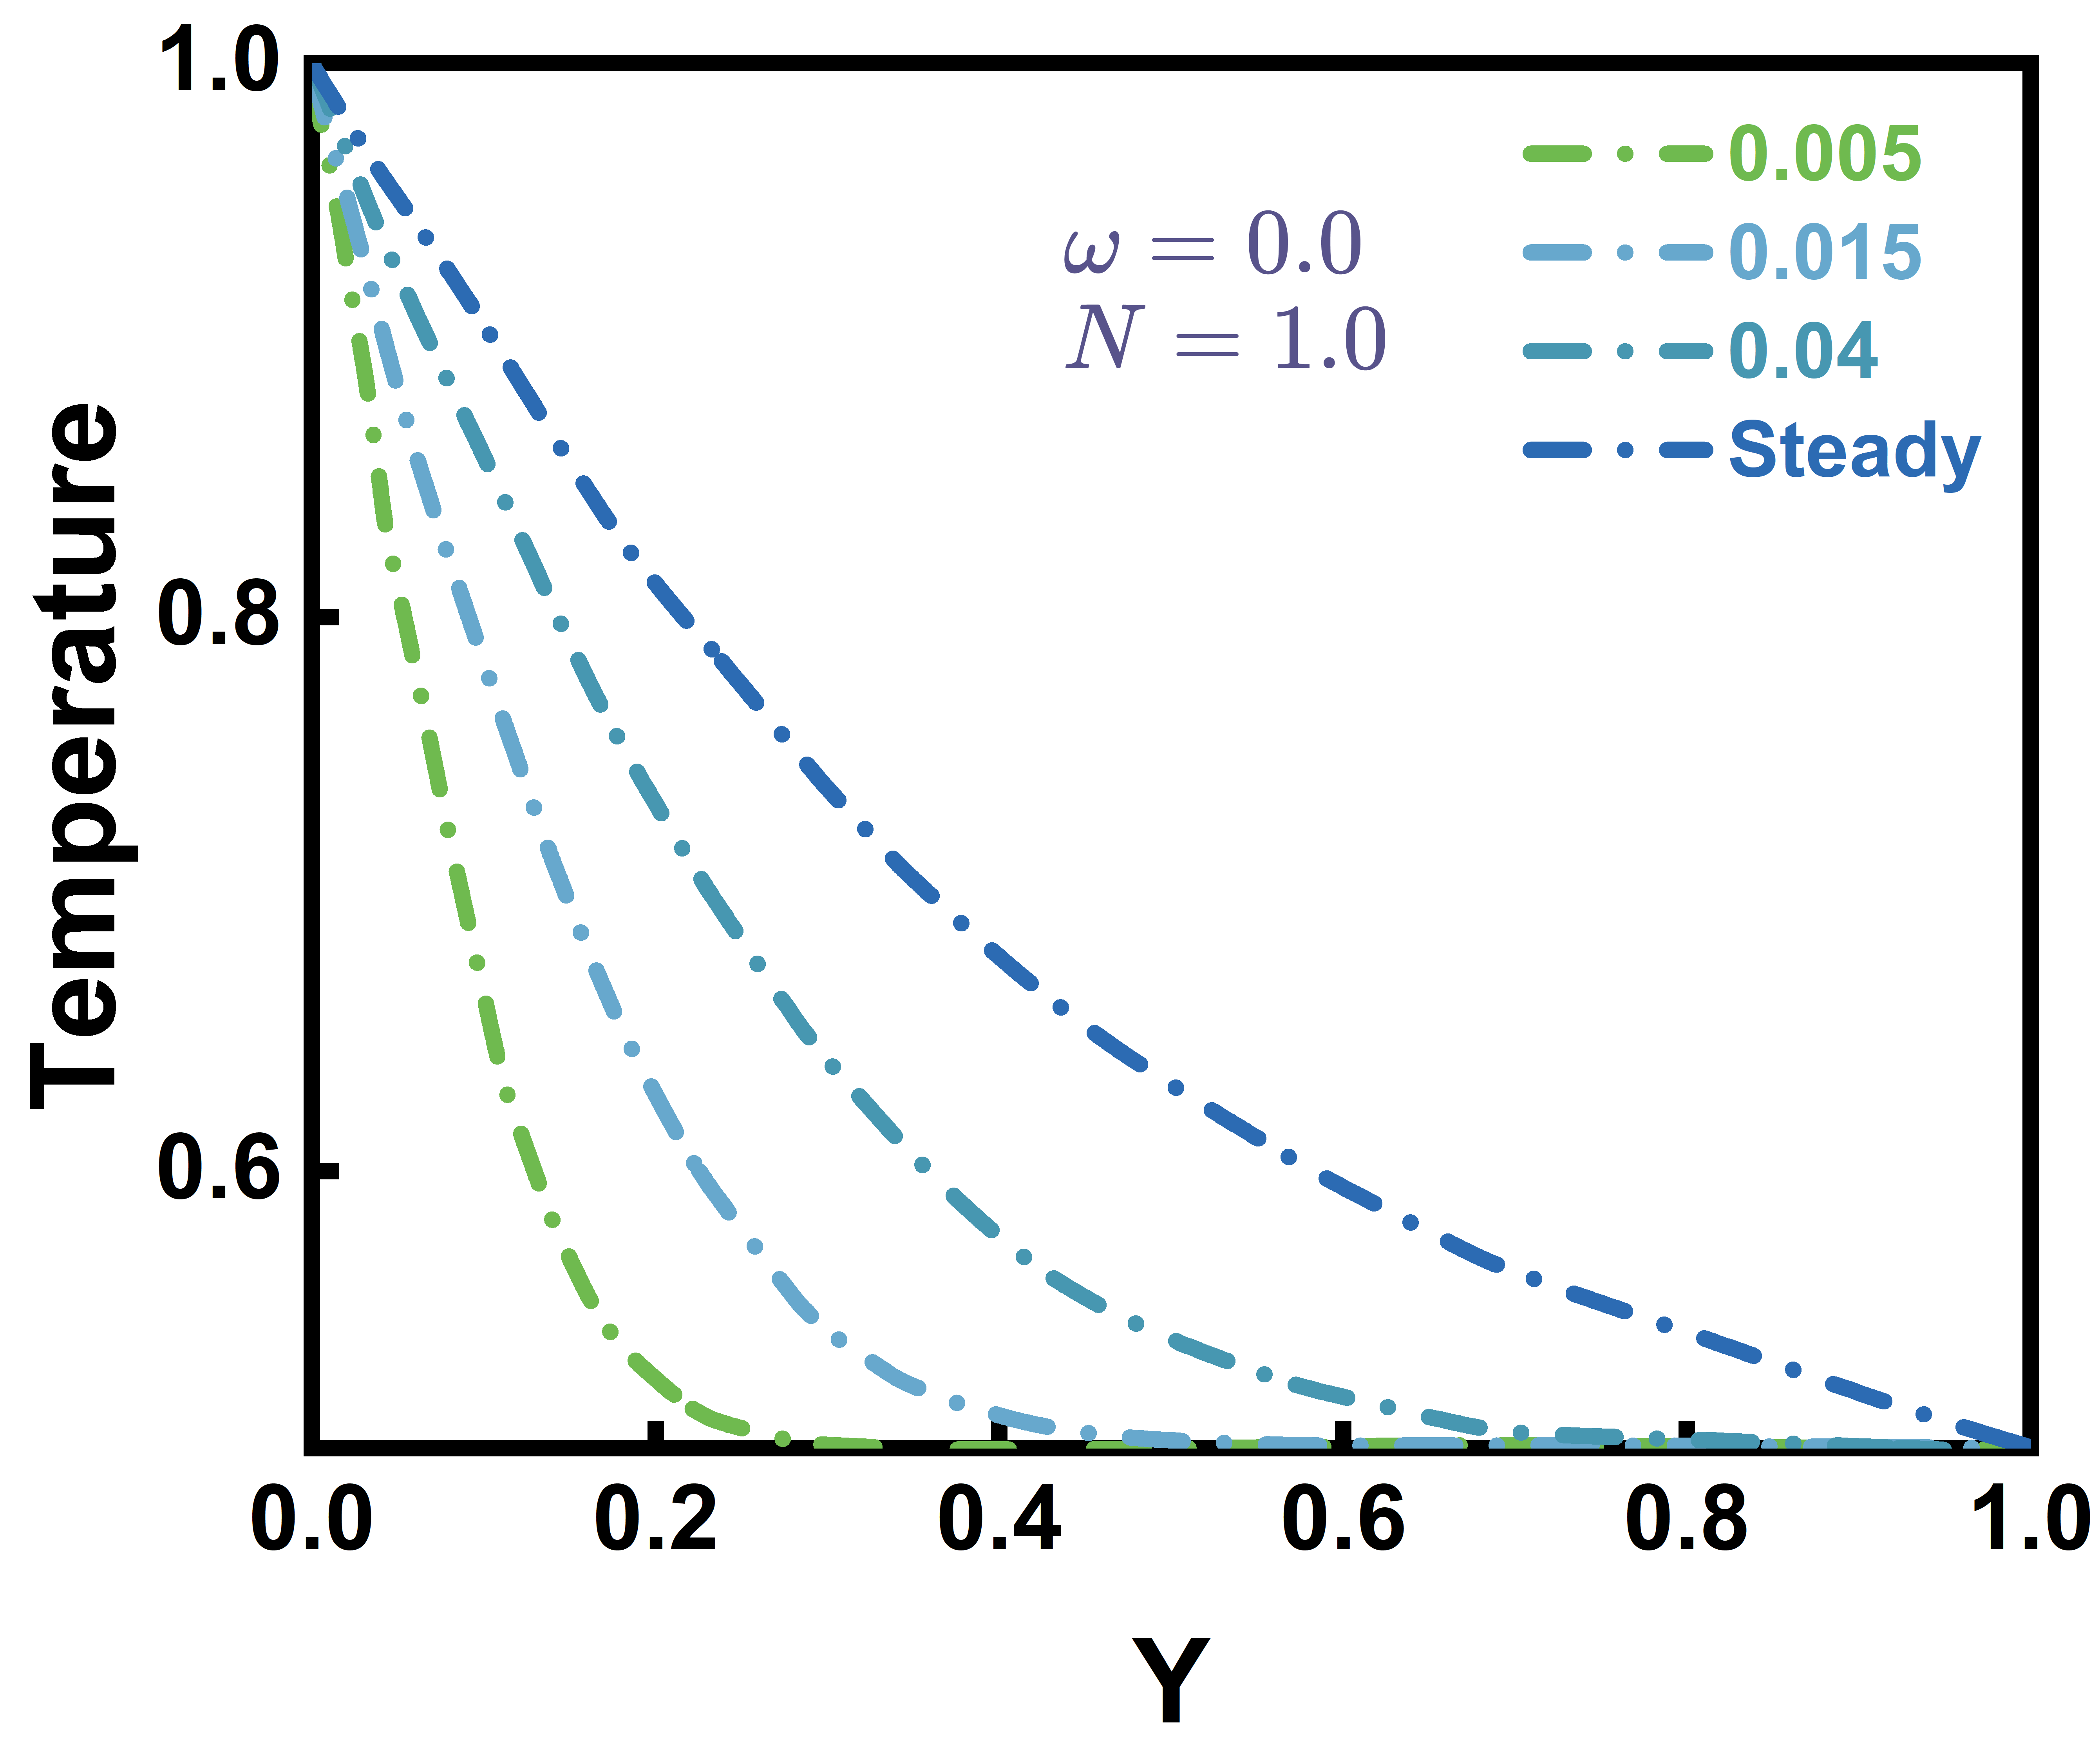
\includegraphics[width=\textwidth]{7C.png}
\caption{}
\end{subfigure}
\caption{Transient centreline temperature profiles in the two-dimensional square enclosure at $\omega=0$. The conduction--radiation parameter is (a) $N=0.01$, (b) $N=0.10$, (c) $N=1.00$.}
\label{fig7}
\end{figure}

Figure~\ref{fig7} shows centreline temperatures at $\omega=0$ for different values of $N$. At $N=0.01$, most of the medium heated rapidly, including at early dimensionless times. At $N=1.00$, early temperature changes remained concentrated near the south wall. Increasing $N$ lowered the centreline temperature and reduced thermal penetration into the upper enclosure. At steady state, the north-wall temperature gradient was larger for smaller $N$.

\section{Discussion}
\label{sec:discussion}

The benchmark comparisons indicate that the coupled DUGKS resolves transient conduction--radiation exchange consistently in both planar and square media. It recovered the nonlinear temperature and decomposed heat-flux behaviour reported for the one-dimensional slab~\cite{Talukdar2001}. It also reproduced the centreline behaviour of the two-dimensional LBM--FVM benchmark~\cite{Sun2016}. Agreement across both geometries supports the use of one finite-volume kinetic framework for the energy equation and RTE.

The principal numerical contribution is the common DUGKS structure used for conduction and radiation. A kinetic representation advances temperature, while pseudo-time relaxation resolves the angular intensity. Both equations use characteristic interface reconstruction on the same control-volume grid. The radiative source is therefore evaluated directly at temperature nodes without inter-mesh interpolation. This alignment is particularly useful when $G$ and the nonlinear emission term $\theta^4$ change during every physical time step.

The parametric trends reflect two distinct controls on energy exchange. Increasing scattering albedo redirects more radiation without converting it into material energy, which weakens volumetric heating. The resulting temperature is lower, and the transient lasts longer. Increasing $N$ instead reduces the radiative source relative to thermal diffusion. The response consequently approaches the conduction-dominated limit. The same trends in both geometries suggest that the coupling preserves the expected balance among diffusion, emission, absorption, and scattering.

Angular convergence depended on the reported quantity. Temperature changed little beyond $N_\phi=8$, whereas heat flux retained visible angular-discretisation errors. This difference arises because radiative heat flux is the first angular moment of intensity. Flux prediction therefore requires a finer representation of directionality than temperature prediction. Convergence tests based only on temperature may consequently underestimate the angular resolution required for coupled heat-transfer analysis.

The present evidence is bounded by the benchmark assumptions. The calculations considered gray media, isotropic scattering, constant properties, unit optical thickness, and regular planar or square geometries. They do not establish performance for non-gray radiation, anisotropic scattering, strongly temperature-dependent properties, or complex boundaries. Spatial errors, solver tolerances, and the cost of pseudo-time radiation iteration were not quantified. Extensions to nonuniform or unstructured grids will require separate tests of angular accuracy, nonlinear convergence, conservation, and efficiency.

\bibliographystyle{unsrt}
\bibliography{ref}

\end{document}
